%%This is a very basic article template.
%%There is just one section and two subsections.
\documentclass[12pt,a4paper,spanish,openany]{book}
\usepackage{anysize}
%marginsize{left}{right}{top}{bottom}:
\marginsize{3cm}{2cm}{2cm}{2cm}

% Set equal left margins on book style
\setlength{\oddsidemargin}{0cm}
\setlength{\evensidemargin}{0cm}


% Utilizamos el paquete para utilizar español
\usepackage[spanish]{babel}
% Utilizamos el paquete para gestionar acentos
\usepackage[utf8]{inputenc}
% Utilizamos el paquete para gestionar imágenes jpg
\usepackage{graphicx}
\usepackage{enumerate}
\usepackage{verbatim}
\usepackage{chngcntr}
\usepackage{setspace}

\usepackage{booktabs}
\usepackage{rotating}
\usepackage{hyperref}
\hypersetup{
colorlinks = false,
linkbordercolor = {1 1 1},
citebordercolor = {1 1 1},
urlbordercolor  = {1 1 1}
}

%\doublespacing
%\singlespacing
%\onehalfspacing
%For other sizes use the \setstretch command like this:
%\setstretch{1.8}

\usepackage[acronym]{glossaries} % make a separate list of acronyms
% to use call
% $> latex choco-doc
% $> makeglossaries choco-doc
% $> latex choco-doc

\makeglossaries





\newglossaryentry{2D}
{name=2D,
description={to be define}
}

\newglossaryentry{3D}
{name=3D,
description={to be define}
}

\newglossaryentry{hardware}
{name=hardware,
description={to be define}
}

\newglossaryentry{software}
{name=software,
description={to be define}
}

\newglossaryentry{offline}
{name=offline,
description={to be define}
}


\newglossaryentry{plug and play}
{name=plug and play,
description={to be define}
}

\newglossaryentry{applets}
{name=aplets,
description={to be define}
}


\newglossaryentry{scripts}
{name=script,
description={to be define}
}

\newglossaryentry{on demand}
{name=on demand,
description={to be define}
}

\newglossaryentry{framework}
{name=framework,
description={to be define}
}

\newglossaryentry{JNDI}
{name=JNDI,
description={to be define}
}

\newglossaryentry{GET}
{name=GET,
description={to be define}
}

\newglossaryentry{POST}
{name=POST,
description={to be define}
}

\newglossaryentry{RPC}
{name=RPC,
description={to be define}
}


\setcounter{secnumdepth}{3}
\setcounter{tocdepth}{3}



%\renewcommand{\baselinestretch}{2}
\pagenumbering{arabic}
\pagestyle{plain}



\begin{document}
\sloppy
\doublespacing

\title{}
\author{LUIS MIGUEL ZAVALETA VÁZQUEZ}
\date{25 de AGOSTO del 2011}


\singlespacing

\begin{titlepage}

\begin{center}


% Upper part of the page


\includegraphics[width=0.55\textwidth]{./img/LogoITESM.jpg}

\vspace{4 mm}
{\large Campus Ciudad de México}

\vspace{3 mm}
{\large Escuela de Graduados de Ingeniería y Arquitectura}

\vspace{25 mm}
\begin{Large}
\textbf{TESIS}
\end{Large} 


% Title
\vspace{9 mm}
\begin{LARGE}
{ \bfseries Plataforma cliente-servidor para el desarrollo rápido de
aplicaciones de realidad aumentada}
\end{LARGE}


\vspace{25 mm}
{\large Para la obtención del grado de:}

\vspace{5 mm}
\begin{Large}
\textbf{Maestro en Ciencias de la Computación}
\end{Large}


\vspace{25 mm}

\begin{table}[h]
\begin{center}
\begin{tabular}{l l}

Autor: & Ing. Luis Miguel Zavaleta Vázquez \\

Director: & Dr. Benjamín Hernández Arreguín\\

Sinodal: & Dr. Moisés Alencastre Miranda \\

Sinodal: & Dra. Lourdes Muñoz Gómez \\


\end{tabular}
\end{center}
\end{table}

\vspace{22 mm}

% Bottom of the page
{\large México, Distrito Federal, 17 de abril de 2012}

\end{center}

\end{titlepage}

\newpage

\thispagestyle{empty}
\section*{Dedicatoria}
\vspace{35 mm}

\begin{large}
\noindent 
A mis padres:
\end{large}

\vspace{10 mm}
\begin{Large}
\noindent 
\textbf{Gaudencio y Paula}
\end{Large}

\vspace{10 mm}
\noindent 
Por todo el apoyo brindado durante el transcurso de mi vida, por guiar mis pasos
y enseñarme a ser una persona de bien, pero sobre todo por sostenerme y animarme
a lograr mis objetivos en los momentos en los que mis fuerzas parecían
flaquear.

\noindent 
Los amo, los admiro y siempre estaré agradecido por tener la dicha de ser su
hijo.

\vspace{25 mm}
\begin{large}
\noindent 
A mis hermanos:
\end{large}

\vspace{10 mm}
\begin{Large}
\noindent 
\textbf{Juan Carlos y Héctor}
\end{Large}
\vspace{10 mm}

\noindent 
Por su amistad, su cariño, y por la fuerza que ambos tienen y que les permite
superar todas las adversidades, con su valor y su ejemplo me impulsan a ser un
mejor ser humano.





\newpage
\thispagestyle{empty}
\section*{Agradecimientos}

\vspace{35 mm}

\begin{large}
\noindent 
Al Dr. Benjamín Hernández Arreguín
\end{large}

\vspace{5 mm}
\noindent 
Por su apoyo, su paciencia, sus enseñanzas, por compartir
conmigo sus ideas y conocimientos y por haber sido una pieza fundamental para el desarrollo del
presente trabajo.

\vspace{25 mm}

\begin{large}
\noindent 
A la Dra. Lourdes Muñoz Gómez y el  Dr. Moisés Alencastre Miranda.
\end{large}

\vspace{5 mm}
\noindent 
Por su ayuda, sus consejos y sus correcciones que permitieron mejorar el
presente documento.



\newpage
\setlength{\parskip}{\baselineskip} 
\thispagestyle{empty}
\section*{Resumen}

La evolución de los dispositivos móviles ha hecho que sea posible tener en un
solo dispositivo todos los artefactos necesarios para el desarrollo de
aplicaciones de realidad aumentada, esto ha generado un mercado potencial amplio
y con proyección a futuro para empresas y desarrolladores que ofrezcan
aplicaciones de realidad aumentada.

Actualmente existen dos formas diferentes por medio de las cuales se desarrollan la mayoría de las
aplicaciones de realidad aumentada: plataformas de aplicaciones con un API de
desarrollo y librerías para el desarrollo de aplicaciones de realidad aumentada.
Con las primeras es posible generar aplicaciones de forma rápida, sin embargo no
permiten a los desarrolladores agregar o modificar características, ni optimizar
sus componentes, esto dificulta adaptarlo a necesidades específicas. La
segunda opción, en conjunto con otras herramientas permite el desarrollo de
aplicaciones a la medida, pero a cambio requiere de conocimientos en diversas áreas e implica el uso de un
gran numero de recursos.

La presente investigación se realizó con el objetivo de encontrar una
metodología y generar una plataforma que permita aprovechar lo mejor
de ambos mundos, esto con el fin de facilitar la realización  rápida de
aplicaciones de realidad aumentada sin sacrificar la flexibilidad al momento de
implementar características personalizadas. Para lograr el objetivo nos basamos
en tres pilares fundamentales: La división de la aplicación en componentes
independientes, el uso de estándares y la utilización de metodologías de
desarrollo ágil.

Se lograron identificar diversas tecnologías que nos permitieron satisfacer los
objetivos planteados y se propuso un marco de trabajo que facilita el desarrollo
rápido de aplicaciones de realidad aumentada. 

El marco de trabajo propuesto permitió disminuir considerablemente los tiempos
de desarrollo, debido a que evita la realización de actividades mecánicas y
configuraciones innecesarias. Permite a los desarrolladores crear aplicaciones
rápidamente y modificar u optimizar componentes específicos, dejando al sistema implementar las funcionalidades de las otras áreas. También permite
enfocar los recursos en la implementación de la lógica de negocio.




\setstretch{1.15}
\tableofcontents
\singlespacing


\chapter{Introducción}
El objetivo de este capítulo es explicar las razones por la cuales
se decidió llevar a cabo este trabajo de investigación y ubicarlas en
el contexto adecuado.

\section{Antecedentes}

Diversas investigaciones para la creación de aplicaciones que toman datos del
mundo real como base de partida se han estado realizando recientemente
(\cite{Said:2010:PTC:1869652.1869665},
\cite{Taherkordi:2009:SLA:1554233.1554244},
\cite{Rahmani:2010:TCA:1869652.1869662}, \cite{Fujii:2009:SCD:1516533.1516536}).
Esta área ofrece un gran potencial de negocios debido a que los usuarios de
dispositivos móviles desean acceder a contenido multimedia y a servicios
dependientes del contexto desde sus dispositivos móviles
\cite{Davidyuk:2004:CMM:1052380.1052410}, gracias ha esto a aumentado la demanda
de aplicaciones que toman datos del mundo real sin que sea necesario que los
usuarios los especifique explícitamente. 

Los datos obtenidos del contexto no siempre son suficientes, debido a esto surge
la necesidad de obtener datos adicionales acerca de los elementos con los
cuales se esta interactuando, dicha información es comúnmente  obtenida por
medio de sistemas digitales de información.

Las aplicaciones que permiten combinar información virtual con elementos del
mundo real para la creación de una realidad mixta en tiempo real se les conoce
como aplicaciones de realidad aumentada.

Según la definición de Azuma para que una aplicación sea considerada como de
realidad aumentada debe cumplir con tres características: combinar objetos reales
y virtuales, ser interactiva en tiempo real y estar registrada en
3D \cite{Azuma97asurvey}.

Diversos investigadores se han interesado en la realización de aplicaciones de
realidad aumentada debido a que aumenta la percepción y la interacción con el
mundo real y potencializa y mejora la productividad en tareas del mundo real.
\cite{Azuma:2004:OAR:1103900.1103926}.

Hoy en día se cuenta con dispositivos móviles avanzados (llamados teléfonos
inteligentes), los cuales facilitan la implementación de aplicaciones de
realidad aumentada al venir equipados con diversos artefactos como pantallas de
alta resolución, cámaras, acelerómetros, sistemas de posicionamiento global
(GPS), brújulas, etc. \cite{bb86741} además de que sus procesadores gráficos
cada vez tienen mayor poder de cómputo, estas características permiten que
dichos dispositivos sean útiles en la realización de aplicaciones de realidad
aumentada, con la ventaja adicional de tener una alta disponibilidad, ser menos
costosos y más discretos en comparación con dispositivos usados anteriormente
 \cite{bb86741}.

Actualmente existen diversas aplicaciones de realidad aumentada para
dispositivos móviles como layar \cite{layar} la cual hace uso del GPS y la
brújula para ubicar objetos en una área geográfica, contiene un API para que
usuarios puedan agregar un \emph{layar} el cual se compone de coordenadas
geográficas e información asociada a esta, también permite el reconocimiento
de imágenes por medio de detección de bordes y en la última versión agregar
objetos 2D y 3D asociados. Otra aplicación popular es Wikitude \cite{wikitude},
el cual permite encontrar puntos de interés e información relativa a estos
haciendo uso del GPS, la brújula y el acelerómetro. También existe google
Goggles\cite{goggles}, el cual permitirte hacer una búsqueda en internet de un
objeto físico, esto es posible gracias a que reconoce patrones en las
imágenes y las asocia a un texto lo cual permite hacer una búsqueda.

Estas aplicaciones facilitan la creación rápida de aplicaciones de realidad
aumentada pero las características de estas estarán restringidas, si se desea
crear aplicaciones de realidad aumentada sin estar limitado a un marco de
trabajo específico, se puede lograr por medio de librerías como ARToolKit
\cite{hitl} y Studierstub\cite{IntroStTubeES}, estas librerías nos dan una gran
flexibilidad al momento de realizar las aplicaciones, sin embargo tienen el inconveniente de contar con una curva de
aprendizaje alta y requieren invertir mucho tiempo de desarrollo.

Es por ello que es deseable contar con una plataforma que permita aprovechar
lo mejor de ambos mundos, permitiendo la creación rápida de
aplicaciones y que al mismo tiempo facilite la agregación de características
personalizadas.

Diversas metodologías para la creación rápida de aplicaciones manteniendo la
flexibilidad en la implementación de componentes se han venido
popularizando recientemente, una de ellas es la de convención sobre
configuración, dicha metodología se basa en que sistemas, librerías y
marcos de trabajo deben asumir datos por defecto con el fin de evitar
configuraciones innecesarias, existen \emph{frameworks} populares como Ruby On
Rails y EJB3 que  ya están usando dicho concepto \cite{citeulike:5955149}.

%Para reducir el tiempo total en el desarrollo de una aplicación es importante
%reducir la curva de aprendizaje del marco de trabajo, una forma de lograr
%esto es m

Otro aspecto importante para mejorar la productividad es poder construir
software usando y reusando componentes provenientes de otros sistemas, lo cual
permite reducir la duplicación de esfuerzos
\cite{Perry:1992:FSS:141874.141884}, sin embargo como también mencionan Perry y
Wolf, los componentes de otros sistemas pueden contener ciertas restricciones
con el fin de satisfacer una arquitectura en particular, lo cual podría entrar
en conflicto con otras restricciones del sistema, para esquivar dicha
restricción se propone hacer uso de los principios arquitectónicos REST.

REST, permite ignorar los detalles de la implementación de los
componentes y las sintaxis de los protocolos y se enfoca en los roles de los
componentes, las restricciones de la interacción con otros componentes y la
interpretación de los datos. \cite{restfielding}

El principal inconveniente de generar una metodología nueva es la necesidad de
invertir cierta cantidad de tiempo para dominarla, es posible reducir esa curva
de aprendizaje mediante el uso de estándares de facto en la industria. Las
tecnologías que sin ser legitimadas por un organismo de estandarización son
usadas por un gran número de desarrolladores en diversas aplicaciones se
convierten en estándares de facto, su uso elude la necesidad de aprender una
tecnología nueva, o en su defecto, permite que la tecnología que se requiera
aprender pueda ser útil en otras áreas. Entre los estándares de facto mas
usados por empresas de reciente éxito como google y facebook encontramos
REST(\emph{Represent State Transfer Protocol}) y JSON (\emph{JavaScript Object
Notation}) \cite{estoesgoogle}.


\section{Definición del problema}

La realidad aumentada puede ser usada en diversos campos, entre
algunos de sus usos se encuentran relacionar un lugar físico con un sonido
\cite{hat}, para la creación de piezas mecánicas \cite{rtpr} , para
operaciones, como guías de ensamblaje \cite{rupr}, para aumentar la
sensibilidad humana en cocinas domésticas \cite{sui}, para agregar
descripciones de edificios, obras de arte, etc. 

El aumento en las capacidades de los dispositivos móviles hace que sea
factible utilizarlos en la realización de aplicaciones de realidad aumentada,
esto nos permite tener a un gran número de usuarios no especializados como
clientes potenciales. La venta de teléfonos inteligentes esta creciendo
rápidamente, este año aumentaron 74\% y representan el 24\% de las ventas
totales de teléfonos del segundo trimestre del 2011, mientras que en el segundo
trimestre del 2010 representaban el 17\% \cite{md2011} y en el mismo periodo
del 2009 tan solo el 13.6\% \cite{md2010}. Sin embargo siguen existiendo
algunas limitantes, como la capacidad de almacenamiento la cual es limitada,
esto aunado a la gran cantidad de posibles escenarios, hace necesario el uso de
una arquitectura cliente-servidor para poder almacenar diferentes datos cuando
la aplicación así lo requiera.

Como se comentaba en los antecedentes, ya existen diferentes aplicaciones de
realidad aumentada, las cuales contienen un API que permite a los
desarrolladores interactuar con ellas, sin embargo estas no permiten agregar
características nuevas, o modificar las características existentes, y tampoco
modificar el código fuente, lo cual hace imposible optimizarlos, modificar un
módulo en específico o adaptarlo a necesidades específicas.

Si se decide realizar una aplicación a la medida nos encontramos con el
problema de que el desarrollo de aplicaciones de realidad aumentada con una
arquitectura cliente-servidor requiere de conocimientos especializados en
ciertas áreas como creación de aplicaciones gráficas, optimización de recursos,
creación de aplicaciones distribuidas, bases de datos, lenguajes de programación
para servidores, lenguajes de programación para clientes móviles, etc. En mi
experiencia me he dado cuenta que es difícil encontrar personal experto en todas
estas áreas, eso nos lleva a la necesidad de contar con un grupo de
desarrolladores o dedicar bastante tiempo a dominar todas tecnologías antes mencionadas.

Todos los recursos necesarios hacen que sea difícil para los desarrolladores
independientes y las pequeñas empresas desarrollar aplicaciones propias de
realidad aumentada.

%Otro problema que se tiene es que la generación de objetos 3D consume
%demasiados recursos y el tiempo para generarlos es considerable.

%Tener un registro de todas las actividades que se realizan con una aplicación
%de realidad aumentada nos puede dar una idea de que es lo que necesitan los
%usuarios.

\section{Objetivos}

Proponer un marco de trabajo altamente productivo para el desarrollo de
aplicaciones de realidad aumentada, con una arquitectura cliente-servidor basada
en componentes, que proporcione un entorno de desarrollo estandarizado, que
oculte gran parte de los detalles de configuración a los desarrolladores y que
permita usar, modificar o reemplazar fácilmente sus componentes de forma
independiente.

Para el desarrollo se utilizarán tecnologías emergentes para el desarrollo de
aplicaciones.


Otras de las características con las que debe cumplir el marco de trabajo son:

\begin{itemize}
  \item Desplegar información relacionada en
  forma de árbol, con el fin de mostrar los datos obtenidos por medio de
  sistemas digitales de información, la estructura en forma de
  árbol permite identificar fácilmente las relaciones entre los
  diferentes segmentos de información.
 % \item Obtener información de un servidor y relacionarlas con objetos por
  %medio menús.
  \item Proveer de un algoritmo que permita la rápida identificación de
  información relacionada a un patrón, la identificación de información es un
  proceso que tiene que ser realizado de forma serial en tiempo real, por lo
  cual es necesario que sea lo más rápido posible.
 
 \item Tener un servicio web que permita asociar marcadores, datos y objetos,
 y sincronizarlos con la aplicación móvil, para agregar información adicional a
 objetos reales es necesario contar con un indicador en el mundo real que
 nos diga cuando y donde desplegar la información virtual. ARToolKit utiliza con
 este fin imágenes bidimensionales conocidas como marcadores, las cuales
 permiten calcular en tiempo real la posición y la orientación relativa de la
 cámara, en el presente trabajo la información adicional consistirá en un objeto
 3D y datos que serán desplegados en los menús.
 
 \item Tener un registro de las actividades que se realizan con la aplicación
 que permita la obtención de reportes que faciliten el análisis del
 comportamiento de los usuarios.
 
 \item Creación y destrucción de objetos que requieran gran uso de recursos
 basados en geoposicionamiento y pseudo-geoposicionamiento. En un dispositivo
 con recursos limitados es vital disponer de un algoritmo que nos diga
 cuando un dato tiene pocas probabilidades de volver a ser usado para así poder
 eliminarlo. Los actuales sistemas de almacenamiento temporal de datos se
 deshacen de estos cuando llevan un largo tiempo sin ser usados, o cuando la
 frecuencia de uso es baja, el contar con meta-información que indique la
 ubicación física en donde van a ser usados los objetos y la posición actual del
 usuario, permite mejorar dichos algoritmos.
 
 
 \item Utilización del procesador gráfico para agregar texto sobre los
 menús: la creación y procesamiento de imágenes es una tarea que consume muchos
 recursos y tiempo cuando es ejecutada en el procesador central, sin embargo el
 procesador gráfico nos permite realizar estas tareas de forma rápida y
 eficiente.
  
\end{itemize}

Para validar el funcionamiento adecuado se sus características se creará una
aplicación usando dicho marco de trabajo.


\section{Justificación}

El número de aplicaciones de realidad aumentada usadas de manera cotidiana es
relativamente pequeño, sin embargo es un mercado que no deja de crecer, a pesar
de ello pocas empresas invierten en la creación de nuevas aplicaciones y las
que deciden invertir crean aplicaciones muy especializadas debido
principalmente a las complejidades y a las diferentes áreas de conocimiento
que se necesita dominar.

Hoy en día existen un gran número de marcos de desarrollo, lenguajes de
programación, tecnologías, arquitecturas y su número crecen día a a día, esto
aumenta aún más la complejidad del desarrollo de software y hace que sea difícil
para desarrolladores independiente y pequeñas empresas crear una aplicación a la
medida que satisfaga sus necesidades.

El uso del marco de desarrollo propuesto pretende afrontar algunas de las
limitaciones frecuentes con las que se enfrenta un desarrollador independiente o
una micro empresa al momento de desarrollar aplicaciones de realidad aumentada.
Las limitaciones que se pretende resolver son las siguientes:

\begin{itemize}
  \item Falta de experiencia en todas las tecnologías usadas para el desarrollo
  de aplicaciones de realidad aumentada: Esto se tratará creando un marco de
  trabajo que permita el desarrollo de aplicaciones de realidad aumentada basada
  en componentes completamente funcionales en minutos, y que permita a los
  desarrolladores con conocimiento en una tecnología específica modificar un
  componente sin afectar el funcionamiento de los otros.
  
  \item Requiere invertir una gran cantidad de tiempo en el desarrollo
  de la aplicación: El desarrollador podrá ignorar los detalles de implementación y
  configuración de uno o varios componentes, lo que permitirá que enfoquen
  sus esfuerzos y tiempo solamente en las áreas de su interés.
  
  \item Curva de aprendizaje elevada necesaria para aprender un nuevo marco de
  trabajo: Se utilizarán tecnologías ampliamente usadas en la industria, lo que
  disminuirá la probabilidad de que el desarrollador necesite obtener
  conocimientos nuevos.
  
  \item Incapacidad o lentitud en la realización de actividades que requieran
  una gran cantidad de procesamiento: El cliente simplemente hará una petición
  al servidor, en donde se realizarán los procesos que requieran una gran
  cantidad de recursos de forma asíncrona.
  
  \item Falta de conocimiento de los patrones de comportamiento de los usuarios:
  Módulo del lado del servidor que permitirá analizar los patrones de
  comportamiento de los usuarios, esto posibilitará la obtención de datos útiles
  para el mejoramiento y la optimización de las aplicaciones y/o datos relevantes
  para el negocio.
  
  \item Memoria limitada en los dispositivos móviles: El servidor guardará la
  mayoría de los datos, proveerá los datos que requiera el cliente y los
  actualizará cuando sea necesario. También se creará un módulo ligero de
  caching que permita la creación, eliminación y almacenamiento temporal de
  objetos tanto de las formas clásicas como basado en geolocalización.
  
  
\end{itemize}





%Lo que se pretende con este trabajo es crear una plataforma que permita a los
%usuarios crear aplicaciones de realidad aumentada de forma rápida, sencilla y
%ocultando los detalles de implementación y configuración que no son de su
%interés, pero que al mismo tiempo deje que los
%desarrolladores especializados puedan adaptar, modificar, optimizar o
%reemplazar los componentes existentes o agregar componentes nuevos sin la
%necesidad de tener que modificar o entender otros componentes.

Todo esto permitirá que usuarios finales, desarrolladores
independientes, pequeñas empresas y otras personas con diversos perfiles
técnicos puedan crear aplicaciones de realidad aumentada que se adapten a sus
necesidades, sin la necesidad de invertir demasiados recursos en ello.


\section{Hipótesis}
La creación de una plataforma que permita el desarrollo de aplicaciones de
realidad aumentada con una arquitectura cliente-servidor basada en componentes,
utilizando estándares de facto, metodologías de desarrollo ágil y tecnologías de
desarrollo emergentes permitirá a desarrolladores independientes y
pequeñas empresas la creación rápida de aplicaciones que satisfaga
sus necesidades y al mismo tiempo dará la oportunidad a desarrolladores
especializados de adaptar, modificar, optimizar o reemplazar los
componentes existentes o agregar componentes nuevos sin la necesidad de tener
que entender otras áreas.

\section{Metodología}

La recopilación de información necesaria para el presente documento se hará
basada en investigaciones bibliográficas, las fuentes de donde se llevará a
cabo las investigación serán las siguientes:
\begin{itemize}
  \item Biblioteca del ITESM.
  \item Biblioteca digital del ITESM.
  \item Foros de internet especializados.
  \item Libros obtenidos de plataformas digitales.
\end{itemize}

Para el desarrollo de la aplicación se seleccionarán entre diversas
tecnología ampliamente usadas las que mejor se adapten a las necesidades del
sistema.

Para la el modelado de la plataforma se utilizará el estándar ISO/IEC 19501:2005
mejor conocido como UML ( \emph{Unified Modeling Lenguage}).

Se documentará  el desarrollo del prototipo con el fin de obtener
datos que sirvan para comparar la realización de una aplicación usando
directamente la tecnología contra el uso del framework cuando se realice la
implementación de esta.

Se desarrollará un  prototipo de aplicación utilizando la plataforma propuesta
con el fin de probar que cumpla con las características deseadas. Se documentará
el proceso de desarrollo.

En caso de encontrar incoherencias o resultados negativos parciales se
replanteará la hipótesis.


\section{Conclusiones}
Durante este capítulo se definió el problema dentro de un contexto general, se
identificaron los objetivos del trabajo y se estableció una hipótesis de como
podría ser resuelto, también se dio a conocer la metodología que se utilizará
para tratar de probar la hipótesis.

En los siguientes capítulos se hará una investigación bibliográfica de las
tecnologías, se propondrá una arquitectura, se harán pruebas para
comprobar el grado de éxito y se publicarán las conclusiones.





\chapter{Estado del arte}

Los principios de la realidad aumentada (RA) datan de 1962 cuando
Morton Heilig crea un simulador de moto con sonidos, imágenes, vibración y
olores, a partir de ese momento se han creado decenas de aplicaciones para
diversos usos, hoy en día la palabra RA normalmente se usa
para definir una escena del mundo real la cuál es enriquecida con información
adicional relacionada, en la mayoría de los casos con ayuda de elementos
visuales \cite{geopointer}, aunque no esta limitada a lo visual, existen
algunas investigaciones que utilizan el tacto,
olfato \cite{Kaye:2004:MSA:962342.964333} o  audio \cite{hat}. Existen otras
áreas de investigación de las cuales se ha alimentado la RA tales como la 
virtualidad aumentada, la computación ubicua, y la interacción
computadora-humano \cite{1698266}.

Las formas tradicionales para la visualización de aplicaciones de realidad
aumentada durante más de 40 años ha sido por medio de dispositivos de video y
por medio de \emph{head mounted displays} \cite{183317} (HMD)
\cite{Bimber:2007:MAA:1281500.1281628}. El
procedimiento más común es adquirir una imagen,
identificar la existencia de un objeto en específico, separar el objeto del
resto de la imagen, identificar los contornos, calcular la matriz de
traslación para el objeto virtual, esta matriz se aplica sobre la imagen
obtenida previamente, finalmente se despliega el objeto virtual sobre la imagen
adquirida previamente \cite{aroasf}. Para desplegar las imágenes formadas se usa
una serie de componentes ópticos, electrónicos y mecánicos que despliegan la
imagen  dentro del campo visual del observador, en algún lugar entre su ojo y
el objeto físico que será aumentado, dependiendo del dispositivo usado, la
imagen puede ser formada en un plano o en una superficie no-planar más compleja
\cite{Bimber:2007:MAA:1281500.1281628}

%Existen diversos componentes de software que permiten dibujar objetos
%virtuales sobre imágenes, OpenGL es de las mas comunes, además de que existen
%varia bibliotecas basadas en este. \cite{klimt} \cite{hitl}, estas librerías
%hacen uso del procesador gráfico (GPU) para dibujar los objetos virtuales.


Se ha explotado el uso de la realidad aumentada en un gran número de
disciplinas como militar, médica\cite{mrigd},
infraestructura\cite{1527367}, robótica\cite{vhli} \cite{rmac}, videojuegos,
etc.

%Audio
Es posible mejorar la experiencia de los usuarios en actividades cotidianas
agregando sonidos que interactúen con ellos de forma pasiva o activa, para esto
es necesario contar con algún tipo de sensor que indique la posición de los
usuario y dispositivos que emitan el audio adecuado. Existen diversos usos que
se les puede dar a aplicaciones de audio de realidad aumentada, de forma
pasiva puede informar a los usuarios cuando ocurran ciertos eventos como tener
un correo electrónico nuevo, el inicio de una junta, recordatorios de
actividades, etc. De forma activa puede servir como audio guías en museos,
exposiciones, oficinas de turismo, restaurantes, hoteles, etc.

Entre las aplicaciones que hacen uso del audio como principal herramienta para
aumentar la realidad podemos encontrar la descrita en el trabajo de Benderson
\cite{Bederson:1995:AAR:223355.223526}, la cual permite a los visitantes de un
museo acceder a la descripción de piezas de arte cuando camina cerca de ellas
empleando un \emph{minisdisc} modificado, un microprocesador y un receptor de
infrarrojo. Este sistema también detecta patrones de comportamiento con el fin
de proveer información útil, por ejemplo, si una persona visita varias piezas
del mismo artista, el sistema provee de información sobre este. Rozie \cite{hat} en su
investigación titulada
\emph{Hear and There: An Augmented Reality System of Linked Audio}, creó un
prototipo para sobreponer sonidos asociados con un lugar en un espacio físico.
Uno de los aportes relevantes de esta investigación es que permite identificar
la posición del usuario con relación a objetos del mundo real, por ejemplo si se
encuentra de frente o de espaldas, para poder tener todas esas características
hace uso de un conjunto de herramientas, entre las cuales se encuentran un GPS,
una computadora móvil, audífonos, un brújula digital y una \emph{PalmPilot}.

\begin{figure}
\begin{center}
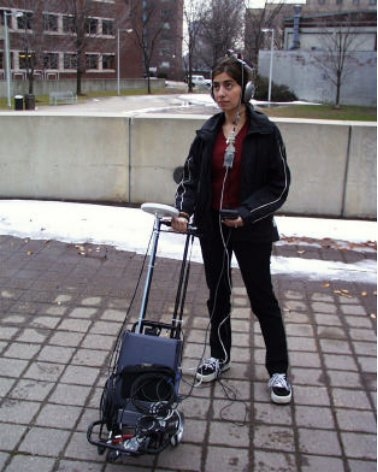
\includegraphics[width=0.5\textwidth]{./img/hearthere.jpg}
\caption{Kit de herramientas usado en Hear and There}
\end{center}
\end{figure}



También es posible utilizar el olfato como medio para aumentar la realidad, los
olores tienen diversos usos en el mundo real, nos indican si es seguro probar
ciertos alimentos, si existe alguna fuga de gas, si un objeto esta limpio, etc,
sin embargo su uso en aplicaciones de realidad aumentada es escaso, esto es
debido a la dificultad para crear olores de forma artificial y a que
existen pocos dispositivos comerciales que permitan controlar y emanar olores.

Kaye realizó una investigación para la creación de aplicaciones de realidad
aumentada usando el olfato  \cite{Kaye:2004:MSA:962342.964333}, entre los
principales descubrimientos obtenidos están los siguientes:
\begin{itemize}
  \item Son útiles solo cuando se ejecutan movimientos lentos con datos de media
  duración.
  \item Los usuarios son más propensos a distinguir calidades de olores, no
  cantidades.
  \item Se debe tener en cuenta que los ingredientes usados para la creación de
  los olores no causen reacciones alérgicas.
  \item Se debe de tomar en cuenta que pueden existir reacciones diferentes al
  mismo olor dependiendo de la cultura.   
\end{itemize}


%Vista
La vista ha sido el principal medio usado para la creación de aplicaciones de
realidad aumentada, existen una diversa cantidad de dispositivos usados para
desplegar la información virtual, los cuales podemos clasificar en las siguientes
categorías: visores adheridos a la cabeza, visores ópticos
espaciales(\emph{Spatial Optical Displays}) y visores portátiles.

Los visores adheridos a la cabeza se pueden clasificar en visores
retinares, HMD y proyectores adheridos a la cabeza.


En aplicaciones de realidad aumentada los HMD han sido usados para sobreponer
imágenes virtuales en escenas reales con ayuda de dispositivos
ópticos \cite{Yokokohji:2000:AIO:832288.835786}, diversas
investigaciones han usado HMD para aumentar la realidad, algunos de los
problemas más comunes de usar HMD es que el rango de visión es estrecho y la
movilidad es limitada \cite{Sherstyuk:2009:DLA:1643928.1643982}, además se
debe minimizar la latencia, sobre todo al hacer movimientos rápidos. Diversas
investigaciones han tratado de reducir esos problemas, por ejemplo Yokokohji
propone usar controles de luminosidad independientes, en este trabajo se creó
un algoritmo que hace que en cada ciclo del bucle principal de gráficas cada
fuente de luz se compare con la posición y orientación del usuario, si la
fuente de luz se encuentra enfocada hacia el usuario la intensidad se magnifica
artificialmente. Para diferentes tipos de luz los factores de magnificación se
procesan de forma diferente. También se ha hecho uso de otros dispositivos para
disminuir la latencia sobre todo cuando se ejecutan movimientos rápidos en el
campo de visión, Sherstyuk et al. hicieron uso de un GPS para predecir los
movimientos de la cabeza del usuario y así poder disminuir la latencia y hacer
que el campo de visión sea más robusto.

Otra de las investigaciones sobre HMD es la realizada
por Parviz, la cual basa su artículo \emph{Augmented Reality in a ContactLens}
\cite{arcl}, en la creación de lentes de contacto que permitan agregar
información virtual al mundo real. Para lograr esto se integraron circuitos de
control, comunicación y antenas en miniatura a los lentes usando
optoelectrónicos hechos a la medida, además de agregar información, se
construyeron algunos sensores que pueden detectar la concentración de algunas
moléculas como la glucosa, se prevé que en el futuro sirva para monitorizar los
niveles de colesterol, sodio y potasio entre otros. El primer problema que
encontraron es que muchas de las partes de los lentes y los subsistemas son
incompatibles entre sí, para resolver ese inconveniente se crearon todos los
dispositivos a partir de cero. Otro de los retos el cuál a la fecha de publicación de artículo todavía no se había resuelto completamente fue que
todos los componentes deben de ser miniaturizados e integrados sobre una
superficie de 1.5 pulgadas cuadradas de un polímero flexible y trasparente, se
han logrado avances como el desarrollo de un proceso propio de ensamblaje el
cual les permite integrar diferentes componentes en los lentes. El tercer reto
fue hacer que estos dispositivos no sean tóxicos y puedan usarse de forma
segura, para sobrellevar esto se encapsulo los lentes de contacto en un
polímero biocompatible y se hicieron pruebas en conejos vivos, las cuales
fueron exitosas.
%Para energizar los componentes se planeo crear un sistema que permita
%la recolección de energía inercial del medio ambiente, convirtiendo las
%vibraciones del ambiente en energía o recibiendo energía solar o por medio de
%radiofrecuencias.




Los proyectores adheridos a la cabeza (\emph{Head-mounted Projectors}) (HMP) 
tienen la ventaja de soportar aplicaciones multiusuarios y móviles, tienen el
potencial de combinar las ventajas de los dispositivos de proyección con las de los HMD \cite{Bimber:2007:MAA:1281500.1281628}, uno de
sus defectos es que requiere que la pantalla este en el plano de la imagen.
\cite{Kjlma:2009:FIP:1549820.1549906}, otra desventaja es que cubren
gran parte del rostro, lo que impide la comunicación con otras personas que se
encuentren alrededor. Sonoda et al. proponen un proyector llamado X'tal Visor
que solo cubre una parte de la cara permitiendo así que se pueda entablar
comunicación con otras personas mientras se usa el dispositivo.
\cite{Sonoda:2005:XFO:1187297.1187330}. Este dispositivo consiste en un
proyector con un micro espejo esférico completamente reflejante y una pantalla
retro reflejante para la proyección de las imágenes, primero una imagen
pre-distorsionada es concentrada por unos lentes condensadores, luego el espejo
es colocado cerca del punto focal de los lentes, gracias al uso del micro
espejo esférico la imagen se expande y se distorsiona, al distorsionarse
nuevamente la imagen pre-distorsionada se genera la imagen original.

A diferencia de los HMD, los visores ópticos espaciales
(VOE) separan la mayoría de las tecnologías del cuerpo de los usuarios y los
agregan al medio ambiente, existen tres tipos diferentes de VOE, los cuales
difieren principalmente en la forma en como aumentan la realidad.

El primer enfoque permite visualizar los objetos aumentados a través de un
video, este enfoque es el que ofrece el mejor costo-beneficio cuando no es
necesario tener una aplicación móvil o un dispositivo óptico, la visualización
de la mezcla de objetos virtuales y reales se hace por medio  de un monitor, el
principal problema es que el campo de visión esta limitado al tamaño del
monitor, así como a su resolución. 
%, la mayoría de las aplicaciones de este tipo
%proveen de una vista remota que permite visualizar los.
Diversas investigaciones han usado este enfoque, un ejemplo es la investigación
titulada \emph{Assembly Guidance in Augmented Reality Environments Using a
Virtual Interactive Tool} \cite{agar}, en la cual se crea un sistema el cual
ayuda al ensamblaje de piezas mecánicas, como se muestra en la figura 2.2, para
el reconocimiento de imágenes se hace uso de redes neuronales. Marín et al. también usan esta técnica para el
manejo de robots por medio de internet, en este caso se hizo uso de la RA para
agregar información  basada en conocimientos previos, y así  como poder 'ver'
partes de la herramienta que no son visibles a simple vista.

\begin{figure}
\begin{center}
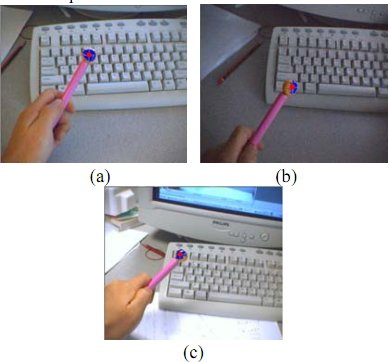
\includegraphics[width=0.5\textwidth]{./img/assemblyGuidance.jpg}
\caption{Ejemplo de seguimiento en tiempo real de una pluma, en una aplicación
funcional se sustituye la pluma por una pieza mecánica y se indica la forma de
ensamblarla con otras piezas}
\end{center}
\end{figure}



El segundo enfoque es ver a través de dispositivos ópticos, estos dispositivos
superponen al medio ambiente con gráficas computacionales de tal modo que las
imágenes virtuales y las imágenes reales son visibles al mismo
tiempo, a diferencia de otros enfoques con este no se siguen los movimientos de
los usuarios, pero a cambio soporta moverse alrededor de
ellos.\cite{Bimber:2007:MAA:1281500.1281628}

El último enfoque se basa en dispositivos basados en proyección espacial, estos
aumentan la realidad directamente, aplicando una proyección frontal que
despliega imágenes directamente sobre la superficie de objetos físicos.
Jackie Chia-Hsun Lee en su investigación titulada
\emph{Spatial user interface: Augmenting Human Sensibilities in a Domestic
Kitchen} hace uso de este enfoque para permitir que un ambiente de cocina sea
mas expresivo y sensitivo para las personas, esto lo logran  proveyendo  información
adicional (visual, audio y otras informaciones sensoriales) con el fin de hacer
que los usuarios de una cocina domestica perciban situaciones anormales
rápidamente, permitiéndoles estar enterados de información
crítica, el objetivo es convertir una cocina en un espacio lleno de colores y
sonidos que indique de una forma fácilmente reconocible lo que está
ocurriendo, para que en caso de que todo esté normal, el usuario se pueda
enfocar en actividades rutinarias, para lograr este objetivo se hace uso de
diversos sensores.


La última categoría de dispositivos usados para aumentar visualmente la realidad
son los visores móviles, los ejemplos tradicionales de los dispositivos móviles
son las tabletas, los asistentes digitales personales (\emph{PDAs}) y
recientemente los teléfonos celulares \cite{Bimber:2007:MAA:1281500.1281628}.
Todos esos dispositivos combinan procesadores, memorias, pantallas y tecnología
de interacción en un solo dispositivo, las cámaras integradas en dichos
dispositivos proveen videos casi en tiempo real, sobre los cuales se le agregan
imágenes virtuales antes de que sean desplegados.

El principal inconveniente en la realización de aplicaciones de RA enfocada a
visores móviles es que tanto el procesamiento como la memoria son relativamente
limitados, una forma común de resolver esta desventaja es realizando las tareas
que requieran procesamiento intensivo de información y guardando los datos que
ocupen mucho espacio en un servidor independiente, y mandar a llamar dicha
información solo cuando sea necesario.


Takacs et al. (ver figura 2.3) crearon un sistema de realidad aumentada para
teléfonos móviles que identifica imágenes provenientes de la cámara de teléfono y busca otras
imágenes relacionadas a esta, para facilitar la búsqueda de imágenes, estas
contienen meta-información que indica su ubicación, esto con el fin de limitar
la búsqueda a imágenes cercanas a la posición del usuario la cual se obtiene a
través del móvil. Las imágenes y su meta-información se encuentran almacenadas
en una amplia base de datos. Se creó un algoritmo robusto que permite la obtención de
imágenes, este algoritmo es el encargado de filtrar las imágenes de la forma
mencionada previamente y también permite su compresión y actualización incremental con lo cuál se
logra reducir la latencia. La detección de imágenes se basa en el algoritmo SIFT
(\emph{Scale-invariant feature transform}), el cual por medio de la detección de
puntos de referencia, permite el reconocimiento de objetos. Dicho algoritmo
se optimizó para que funcionara eficientemente en dispositivos móviles. Dicho trabajo obtuvo buenos resultados, se logró la creación de un algoritmo que consume pocos
recursos, trabaja mediante una arquitectura cliente-servidor y ejecuta
la mayor parte del procesamiento en el lado del servidor.\cite{1460165}

\begin{figure}
\begin{center}
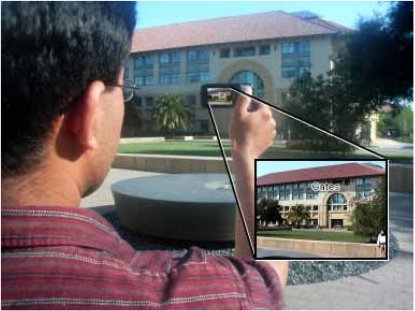
\includegraphics[width=0.5\textwidth]{./img/outdoorsAR.jpg}
\caption{El sistema creado por Takacs aumenta la imagen obtenida por medio de
una cámara de un teléfono con información acerca de los objetos que reconoce}
\end{center}
\end{figure}


Otra investigación parecida es la realizada por Sthephan Gammeter et. al., ellos
presentaron un sistema para realidad aumentada en móviles basado en
reconocimiento visual, este sistema relega las tareas de reconocimiento de
imágenes a un servidor, mientras que el cliente realiza las tareas de
seguimiento. Cuando el cliente detecta un objeto relevante hace una petición a
un servicio de reconocimiento de imágenes, pero no se detiene en espera
de una respuesta, también trata de minimizar las peticiones al
cliente identificando los objetos que ya fueron procesados previamente, para no
mandar peticiones repetidas al servidor. \cite{bb86741}

%En este trabajo se presenta una realidad aumentada
% (AR) del sistema para ayudar a los trabajadores de campo de empresas de
% servicios públicos en las tareas al aire libre, como el mantenimiento, la
% planificación o la topografía de la infraestructura subterránea.

Schall et. al. realizaron una investigación haciendo uso de dispositivos móviles
creados a la medida, el objetivo de la investigación fue crear una herramienta
que ayudara a los trabajadores de campo de empresas de servicios públicos en
tareas al aire libre, como el mantenimiento y la planificación de
infraestructura subterránea. Este sistema logró sobreponer gráficas 3D a
escenarios del mundo real para lograr lo que llamaron Visión de rayos X, esta
característica permite a los empleados ver que existe detrás de las
infraestructuras, también cuenta con un módulo de etiquetado que permite agregar
meta-información a imágenes, otra de sus características es que permite
compartir imágenes entre diferentes dispositivos. \cite{1527367}

Otro trabajo relacionado con teléfonos inteligentes fue el realizado por Beer y
Wolfgang \cite{geopointer}, ellos presentaron un concepto al cual llamaron
\emph{Geopointer} el cual permite a los teléfonos inteligentes actúen como
punteros tangibles con el fin de recibir información acerca de un objeto
del mundo real. Este trabajo permite que al señalar un objeto, el usuario
reciba información contextual acerca de él, para lograr esto es necesario
contar con un dispositivo que permita señalar los
objetos, para este fin se hizo uso de un teléfono celular, el cual por medio de
diversos sensores, permite conocer la dirección a la que esta apuntando el usuario, el principal aporte de esta
investigación es que ofrece una manera intuitiva de seleccionar objetos en el
mundo real. La arquitectura del sistema de GeoPointer consiste de un cliente
ligero y una aplicación en un servidor, en el servidor se procesan
todas las transformaciones y se conecta a un sistema de información geográfica
externo, el cliente obtiene la longitud y la latitud del dispositivo por medio
del GPS, así como su ubicación haciendo uso de la brújula, el teléfono combina
los datos obtenidos por medio de la brújula y la aceleración relativa para
calcular la orientación relativa del dispositivo en un espacio 3D, el cliente
no realiza ninguna operación simplemente manda los datos al servidor, en donde
se hacen todos los cálculos y se regresan los datos obtenidos al cliente para
que despliegue la información.


En el 2008 se liberó al público general Android, y a finales de ese mismo año
se creo el primer dispositivo basado en Android.

El lanzamiento de el sistema operativo móvil de google, Android y el primer
teléfono basado en Android (HTC Dream) permitió que se tuvieran en un solo
dispositivo todos los componentes necesarios para aplicaciones
de RA basadas en geolocalización tales como GPS, brújula, acelerómetro y una
plataforma de desarrollo de fácil acceso\cite{citeulike:6844215}. Esto permitió
que las aplicaciones de realidad aumentada sobre teléfonos móviles pudieran
alcanzar millones de usuarios al mismo tiempo, gracias a esto se crearon
aplicaciones masivas, que actualmente son altamente populares tales como Layar,
Wikitude y Google goggles.


Layar se basa en aplicar información digital sobre objetos del mundo real
vistos a través de una cámara \cite{Eishita:2010:TSA:1920778.1920811}, esto con
el fin de discriminar diferentes tipos de información y darle al usuario la opción
de filtrarla, esta se divide en
capas llamadas \emph{layers}. Los layers pueden ser creados por usuarios por
medio de un archivo XML, aunque también se pueden usar otros formatos como
JSON. La aplicación se divide en 5 componentes básicos: 
\begin{itemize}
  \item Un cliente para el dispositivo móvil.
  \item Un servidor que provee las interfaces de la aplicación y comunicación
  con proveedores de servicios externos.
  \item Un sitio web provisional para que los desarrolladores puedan subir
  nuevos \emph{layers} y administrar sus \emph{layers} y cuentas.
  \item  Un proveedor de servicios creado por los desarrolladores.
  \item Una fuente de contenidos.
\end{itemize}
El servidor es el que se encarga de
procesar los datos y obtener la información, la cual se manda al cliente, usando
el formato JSON. Actualmente están por liberar un complemento llamado layar
visor, esto permitirá reconocer objetos del mundo real, y desplegar información
digital sobre ellos.


Wikitude World Browser es un navegador de propósito general, una de sus
principales características es que cuenta con localización basada en movimiento
y soporte para el despliegue de imágenes 2D, esta basado en Wikitude API, un
marco de trabajo de código abierto para el desarrollo de aplicaciones
\emph{standalone} sobre Android, iPhone y algunos dispositivos basados en
Symbian \cite{madden2011professional}. A partir de la versión 4 liberada en
enero del 2010 ya soporta completamente ARML (\emph{Augmented Reality Markup
Language}). ARML es una propuesta de Mobilizy (la misma empresa desarrolladora de Wikitude) con el fin de estandarizar la
forma de comunicarse de aplicaciones de realidad aumentada, esta actualmente
siendo revisada por el W3C.

Google goggles permite hacer búsqueda por medio de Google usando como dato de
entrada una imagen del mundo real obtenida por medio de la cámara de un
teléfono, reconoce diferentes tipos de objetos, entre ellos lugares, monumentos,
obras de arte, logotipos, etc. También permite el reconocimiento de texto y la
traducción de este de forma automática.


\chapter{Elementos que componen una aplicación de RA}


\section{Introducción}

En el presente capítulo se hará una explicación teórica sobre los elementos
necesarios para la construcción de aplicaciones de realidad aumentada.
En la primera sub-sección se resaltarán los elementos requeridos para el
desarrollo de aplicaciones gráficas, poniendo especial énfasis en las
aplicaciones gráficas interactivas, ya que son éstas las que permiten al usuario
final modificar el comportamiento de una aplicación, se analizarán los tipos de
software y los lenguajes de programación más comúnmente usados, al final se hará una
breve investigación sobre los estándares para el desarrollo de aplicaciones
gráficas.

Posteriormente ser analizarán diversos marcos de trabajo para aplicaciones de
realidad aumentada con el fin de seleccionar el que mejor se adapte al
desarrollo del presente trabajo.


\section{Aplicaciones gráficas}



\subsection{Introducción}

Hasta principios de la década de los 80's las gráficas computacionales eran un
campo pequeño y especializado, principalmente por que las aplicaciones gráficas
fáciles de usar y con una relación costo-beneficio positiva eran pocas,
principalmente por que requerían de equipos  grandes y costosos, sin embargo
debido a los avances en hardware estas desventajas se han ido minimizando, por
ejemplo los monitores han evolucionado desde pantallas hechas a la medida hasta
interfaces humanas estándares para las computadoras, todo esto ha hecho que hoy
en día los gráficos por computadora se hayan convertido en una herramienta útil
y asequible.


%Los avances en hardware han hecho posible la evolución de , lo cual ha
%permitido reducir los costos haciendo mas accesibles las aplicaciones de
%realidad aumentada.
%las primera aplicaciones que usaron gráficos por computadoras

%Los gráficos por computadora son una potente herramienta ayuda en la producción
%de imágenes,

%Los gráficos por computadora hacen uso de diversas áreas como las
%ciencias, las artes, la ingeniería, negocios, industrias, medicinas,
%administraciones públicas, entretenimiento, publicidad, educación y
%aplicaciones caseras, hoy en día incluso se pueden transmitir imágenes a través
%de internet.

Las gráficas proveen una de las formas más naturales de comunicarse con una
computadora, esto es gracias a que los humanos poseemos una asombrosa capacidad
de reconocer patrones \gls{2D} o \gls{3D} de forma rápida y eficiente.

Las gráficas computacionales se enfocan principalmente en el análisis o
reconstrucción de objetos  o modelos 2D o 3D reales o imaginarios e incluyen el
almacenamiento y manipulación de los mismos, se alimenta de
diversos campos incluyendo física, matemáticas, ingeniería, arquitectura, etc.

Existen diferentes formas de categorizar las gráficas computacionales.
\begin{enumerate}
  \item Por tipo (cantidad de dimensiones): Imágenes (2D) u objetos en 3
  dimensiones (3D).
  \item Por tipo de interacción la cual se determina por el grado de
  control que tienen los usuarios sobre los objetos: Despliegue no interactivo
  (la aplicación hace el trazado basado en datos predefinidos) y despliegue
  interactivo (El trazado se hace con una combinación de datos proveídos por el usuario y
  datos predefinidos en el sistema).
  \item Por el rol de la imagen: Si la imagen es el fin en sí misma o sólo un
  medio.
\end{enumerate}


\subsection{Aplicaciones gráficas interactivas}

La mayoría de las aplicaciones gráficas son altamente interactivas, el usuario
controla el contenido, la estructura y la apariencia de los objetos y las imágenes usando
para ello dispositivos de entrada como teclados, ratón, o paneles sensitivos al
tacto sobre la pantalla. Las gráficas computacionales interactivas son la forma
más importante de reproducir imágenes desde la invención de la fotografía y la
televisión, con la mejora de que puede representar no solo objetos del mundo
real sino también objetos abstractos.

El uso de objetos que puedan ser controlados dinámicamente es especialmente útil
cuando el usuario desea controlar la animación, ajustando diversas características como la velocidad, la
cantidad de detalles mostrados, la forma de representación etc. Debido a esto la
mayoría de las aplicaciones gráficas interactivas se componen de un conjunto de
\gls{hardware} y \gls{software} que permite a los usuarios manipular el
movimiento y la actualización de la forma, el color u otras propiedades de los
objetos que están siendo vistos.

El software para aplicaciones gráficas cuenta con tres componentes: un
programa que que crea la aplicación y maneja los datos de entrada de los
usuarios, el modelo de la aplicación el cual representa la información o los
objetos que van a ser desplegados en la pantalla y el sistema gráfico el cual
genera las vistas a partir de una serie de instrucciones que especifican la
descripción geométrica detallada sobre que se debe de ver y como se debe de ver.
%de que se debe de ver como los atributos que especifican cómo se debe de ver.
%Las vistas se producen
%enviando los datos procesados al tercer componente, el sistema gráfico, una
%serie de instrucciones que contienen tanto la descripción geométrica detallada
%de que se debe de ver como los atributos que especifican cómo se debe de ver.
El sistema gráfico es por lo tanto un intermediario entre el programa y la
pantallas. (Ver fig. 3.1 )

La tarea fundamental de un diseñador de aplicaciones gráficas interactivas es
especificar que clase de objetos van a ser generados y representados, y cual va
a ser la forma de interactuar de los usuarios con respecto a la creación y
modificación de los modelos y su representación visual.

\begin{figure}
\begin{center}
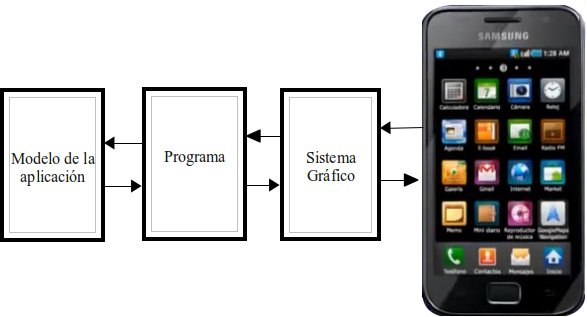
\includegraphics[width=0.5\textwidth]{./img/sistGra.jpg}
\caption{Componentes de una aplicación gráfica}
\end{center}
\end{figure}

El modelo es dependiente de la aplicación e independiente de cualquier
dispositivo en particular, sin embargo el programa debe convertir una porción
del modelo en una representación geométrica que el sistema gráfico pueda
entender para crear la imagen deseada, el proceso de conversión se hace en dos
fases, primero la aplicación obtiene del modelo las porciones que se
visualizarán, después se convierte a un formato que pueda ser enviado al sistema
gráfico, los datos obtenidos del modelo deben de ser figuras geométricas
soportadas por el sistema gráfico o convertirse en estas.

El sistema para manejo de interacciones con los usuarios es un ciclo dirigido
por eventos, se puede visualizar como una máquina de estados finita con un
estado central de espera y las transiciones hacia otros estados son generadas
por eventos creados por los usuarios, como se muestra en el pseudo-código 3.1.


\begin{verbatim}
    while(!cerrar){/*el usuario no ha seleccionado la opción cerrar*/
        permitir la selección de eventos
        switch(selección){
          Procesar la selección, 
          actualizando la imagen cuando sea necesario.
       } 
   }
\end{verbatim}
\begin{center}
Pseudo-código 3.1: Manejo te interacciones en una aplicación gráfica.
\end{center}

%La transformaciones de traslación, rotación y escalado son esenciales para
%muchas aplicaciones gráficas.

Con el fin de manipular los objetos de las aplicaciones gráficas se hace uso de
diversas transformaciones, las cuales son usadas directamente por los programas
por medio de diversas subrutinas, estas permiten modificar las posiciones y las
dimensiones de los objetos en un plano, por ejemplo supongamos que tenemos que
crear una escena de una ciudad, en ese caso se podría usar transformación de
traslación para posicionar objetos que representen señales de árboles y
edificios en los lugares adecuados, la transformación de rotación permitiría
darles la orientación correcta y la transformación de escalado se
usaría para modificar su tamaño.

Uno de los usos relativamente recientes de los gráficos por computadoras
es la creación de aplicaciones virtuales, en la cual los usuarios pueden
interactuar con objetos virtuales en tres dimensiones, gracias a estos sistemas
los usuarios pueden moverse alrededor de los objetos o interactuar con ellos de
diversas maneras, la interacción se hace a través de diversos dispositivos por
ejemplo con guantes especializados.

La creación de imágenes 3D requiere de un proceso más complejo que la creación
de imágenes 2D, esta complejidad extra es debido a dos razones, la primera es
que tenemos que manejar una dimensión adicional y la segunda es debido a que las
pantallas son en 2D. Este problema es solucionado gracias a las proyecciones
que transforman modelos de objetos 3D en proyecciones en un plano 2D como se
muestra en la figura 3.2.

\begin{figure}
\begin{center}
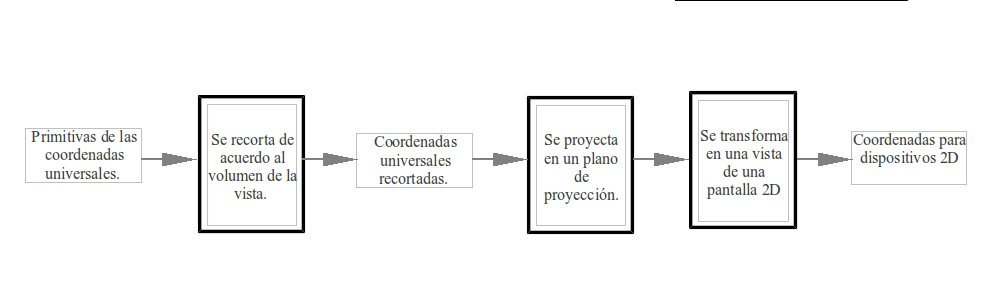
\includegraphics[width=0.9\textwidth]{./img/coord2D3DB.jpg}
\caption{Transformación de modelos 3D a proyecciones 2D}
\end{center}
\end{figure}


%\cite{cgpp-2ed-1995}




%\subsubsection{Dispositivos de entrada y salida}


%Existen diferentes dispositivos de entrada para interactuar con aplicaciones
%gráficas, entre los mas comunes podemos nombrar a los ratones, los cuales son
%pequeños dispositivos que se mueven sobre una superficie plana, y a su vez hace
%que se mueva el cursor en un monitor, trackballs el cual se puede girar con la
%palmas de las manos o con los dedos y que al igual que el ratón genera
%movimiento del cursor, joystick que consiste en una palanca vertical que
%permite mover un cursor, guantes de datos, que contienen sensores que nos
%permites 'agarrar' objetos virtuales, digitalizador que nos permite dibujar o
%seleccionar posiciones de forma interactiva, escáneres que permite hacer una
%copia de una imagen real y almacenarla en un computador, paneles táctiles,
%permiten visualizar objetos o posiciones de pantallas que se pueden seleccionar
%con el toque de un dedo, lapiceros ópticos, son dispositivos en forma de
%lápices que permiten seleccionar posiciones en una pantalla y sistemas de voz
%que permite emtir diversas instrucciones por medio de audio en lenguaje
%natural, que después serán interpretadas por un computador y realizarán una
%acción especifica.

%El dispositivo de salida usado en la mayoría de las aplicaciones gráficas es
%el monitor de vídeo.


\subsection{Software y lenguajes de programación para gráficas
computacionales}


Existen dos tipos de software para la creación de aplicaciones
gráficas, de propósito específico y de propósito general. Los
de propósito específico son usados por personas que no tienen
conocimientos de programación, pero desean generar imágenes, gráficas o
diagramas sin tener que preocuparse de los procedimientos
para producir dichas imágenes, este tipo de aplicaciones funciona por medio de
menús que permite a los usuarios seleccionar diversas acciones usando un
lenguaje basado en su área de conocimiento; un ejemplo de este tipo de
programas es AutoCad, el cual permite entre otras cosas, la creación de planos
de casas y edificios. Los de propósito general, proporcionan una biblioteca con
diversas funciones que pueden ser accedidas usando un lenguaje de programación
como Java, C, C++ u Objetive C, por ejemplo GL, OpenGL, java2D, Java3D, OpenGL
ES, etc, estos sirven como una interfaz entre un lenguaje de programación y el
hardware usado para el procesamiento y despliegue de imágenes.

Para generar una imagen es necesario que se proporcione, mediante un lenguaje de
programación, las descripciones geométricas de los objetos que se van a mostrar,
en dichas descripciones se tiene que especificar tanto la forma como las
posiciones geométricas de los objetos, por ejemplo para describir un cubo se
tienen que especificar la posición de sus vértices, mientras que para una
esfera, basta especificar el centro y el radio. La mayoría de las aplicaciones
gráficas requieren de descripciones geométricas especificadas en un sistema de
referencia de coordenadas cartesianas estándar, algunas aplicaciones especificas
pueden permitir el uso de otro tipo de coordenadas.

Usualmente se utilizan diversas instancias de referencias cartesianas, las
cuales permiten definir objetos individuales de forma independiente, estas se
llaman coordenadas de modelado o coordenadas locales, una vez construidos los
objetos se usa un sistema de coordenadas llamadas coordenadas universales para
colocar dichos objetos en una escena especifica, en este paso se hace una
transformación de las posiciones y las orientaciones de las  coordenadas
locales para adaptarlas al sistema de coordenadas universales. Después de haber
especificado todas las partes de una escena, se ejecuta una serie de subrutinas
que permiten que la escena se visualice en uno o más dispositivos de
salida. En primer lugar las coordenadas universales se convierten a coordenadas
de visualización, después la posición del objeto se transforma para generar una
proyección en un plano 2D, la cual se visualiza en el dispositivo de salida, las nuevas
coordenadas generadas se denominan coordenadas normalizadas, estas coordenadas
normalmente se encuentran en un rango de -1 a 1, o de 0 a 1, esto con el fin
de que sean independientes de los rangos de coordenadas de los dispositivos de
salida. Finalmente se genera un nuevo sistema de coordenadas, el cual es
dependiente del dispositivo, en el cual se muestra la escena, estas se llaman
coordenadas de dispositivos o coordenadas de pantallas, la figura 3.3
especifica este proceso.

\begin{figure}
\begin{center}
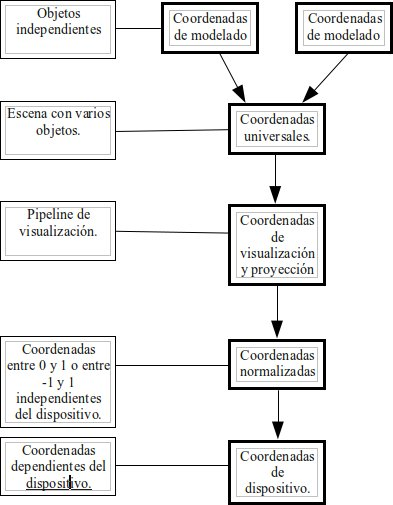
\includegraphics[width=0.5\textwidth]{./img/secuenciaTransformaciones.jpg}
\caption{Secuencia de las transformaciones de coordenadas}
\end{center}
\end{figure}

Se puede alterar el flujo de las aplicaciones gráficas por medio de dispositivos
de entradas, este hecho las convierte en aplicaciones gráficas interactivas,
para manejar los eventos de los usuarios se utilizan funciones de entrada.

\subsection{Estándares de software gráfico}

Existen varios estándares para el desarrollo de aplicaciones gráficas,
normalmente, el objetivo principal de la estandarización es permitir que los
sistemas sean portátiles, cuando se diseñan aplicaciones gráficas basadas en estándares, en
teoría dichas aplicaciones pueden crear varias instancias que corran sobre
diferentes plataformas (hardware) sin la necesidad de modificar el código
fuente. GKS (\emph{Graphical Kernel System}) fue el primer estándar de software
gráfico adoptado por la ISO (\emph{International Standar Organization}) y la
ANSI (\emph{American National Standar Institute}), aunque originalmente el estándar
fue creado para gráficos bidimensionales, pronto se desarrollo una extensión
tridimensional. El segundo estándar ampliamente adoptado fue PHIGS
(\emph{Programmer's Hierarchial Interactive Graphics Standard}), el cual esta
basado en GKS pero soporta el modelado de objetos jerárquicos, especificaciones
de superficie, de color y manipulación de imágenes, después se desarrollo
PHIGS++ el cual contiene mejoras en el soporte de superficies tridimensionales.
Tiempo  después se popularizaron  las estaciones de trabajo gráficas de
Silicon Graphics, las cuales estaban dotadas de un conjunto de rutinas llamadas
GL (\emph{Graphics Library}), esta biblioteca llegó a ser ampliamente usada, al
grado que se convirtió en un estándar de facto. A esto, a principios de
los 90's se creo OpenGL (\emph{Open Graphics Library}), una especificación para
la implementación de versiones de GL independiente del hardware, este estándar no solo se ha mantenido
vigente, sino que se han creado versiones especializadas como OpenGL ES para
dispositivos integrados, y WebGL para navegadores web, OpenGL y todas sus
variantes son mantenidos y actualizados por el Grupo Khronos, el cual esta
compuesto por diversas universidades y empresas de tecnologías como Nvidia,
Intel, HP, IBM, entre otros.

Microsoft creo algunas librerías de OpenGL para que los usuarios pudieran
compilar programas en OpenGL usando Microsoft Visual Studio. A mediados de los
90's Microsoft creó su una API propia para producir aplicaciones en 2D y 3D la
cual llamó DirectX, DirectX es una API propietaria para aceleración gráfica por
medio de hardware sobre sistemas operativos Windows.
\cite{Tan:2008:IDP:1396808.1397457}


\section{Bibliotecas para creación de aplicaciones de RA}

Tres de las bibliotecas más usadas para el desarrollo de aplicaciones de
realidad aumentada son Studierstube, ARToolkit y Qualcomm AR SDK.

ARToolkit es una biblioteca para aplicaciones visuales de realidad aumentada de
de código abierto y multiplataforma, que nos permite agregar objetos 2D ó 3D
reales sobre marcadores, también permite identificar la posición de la cámara
con 6 grados de libertad \cite{Azuma:2004:OAR:1103900.1103926}.

ARToolkit esta compuesto por diversas bibliotecas las cuales tienen un propósito
especifico como:

\begin{itemize}
  \item LibAR: Seguimiento de marcadores.
  \item LibARvideo: Se usa para la captura del video.
  \item LibARgsub:  Usado para dibujar imágenes.
  \item LibARmulti: Seguimiento de marcadores múltiples.
\end{itemize}


%\cite{Azuma:2004:OAR:1103900.1103926}

Studierstube esta basado en ArToolkit, pero contiene características
adicionales. Es una librería multiplataforma soportada por varias versiones
de Windows como XP, Vista, CE y Mobile, también cuenta con soporte para MacOS,
iOS, Symbian y Linux. \cite{StTbEs}

Studierstube cuenta con varias artefactos, cada uno sirve para actividades
específicas, entre los más importantes se encuentran:

\begin{itemize}  
\item Core.
Entre sus principales características está un nivel alto de abstracción,
creación de ventanas, acceso a la cámara, acceso a archivos, creación de redes
por medio de sockets, acceso a audio, temporizadores de alta precisión, y
asignación de variables en tiempo de ejecución.

\item StbMath.
Cuenta con números con punto fijo y con punto flotante, vectores,
matrices, homografía, mínimos cuadrados no lineales %WTH is this? cuaterniones,
entre otros.

\item StbTracker.
Permite el seguimiento rápido de marcadores, típicamente el procesamiento tiene
un tiempo de respuesta de 10ms, maneja diferentes tipos de marcadores.
%entre los cuales
%podemos encontrar marcadores de templates, marcador por frames, matriz de
%datos, split marker, grid marker, ID marker.
\end{itemize}

Qualcomm AR SDK (Ver fig. 3.4) permite la creación de aplicaciones móviles de
realidad aumentada, provee un kit de desarrollo para Android y otro para iOS, las
principales características de Qualcomm AR SDK son las siguientes:

\begin{itemize}
  \item Alto nivel de abstracción para el acceso a las unidades de hardware,
  como la cámara.
  \item Múltiples objetos rastreables.
    \begin{itemize}
      \item Imágenes.
      \item Objetivos múltiples.
      \item Marcadores rectangulares.      
    \end{itemize}
  \item Interacción con el mundo real por medio de botones.  
\end{itemize}


\begin{figure}
\begin{center}
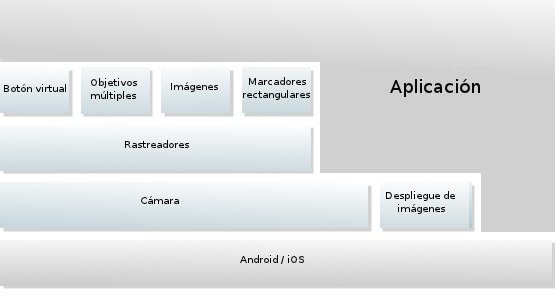
\includegraphics[width=0.75\textwidth]{./img/qcar.jpg}
\caption{Diagrama de alto nivel de Qualcomm AR SDK}
\end{center}
\end{figure}

\section{Conclusión}
Gracias a la primera sección del presente capítulo se pudo identificar que el
estándar actual para la creación de aplicaciones gráficas es OpenGL, por lo
tanto será el utilizado en la realización del presente trabajo, falta
identificar cual es la implementación de OpenGL que se usará y en que versión,
para ello se hará un análisis más detallado en el capítulo 5.

También se analizaron diferentes marcos de trabajo para aplicaciones de realidad
aumentada, el que mejor se adapta a nuestras necesidades es ARToolkit,
principalmente por que uno de los objetivos del presente trabajo es contar con
una herramienta cuyos componentes puedan ser modificados, extendidos o
reemplazados y ARToolkit al ser de código abierto, permite cumplir con esta
restricción sin infringir patente alguna. En capítulos posteriores se analizará
cual implementación se adapta mejor a las necesidades del presente trabajo.




\chapter{Arquitectura basada en componentes}

\section{Introducción}
En el presente capítulo se definirán las razones y las restricciones debido a
las cuales es útil la creación de software utilizando componentes, después se
verán las principales diferencias entre la programación orientada a objetos y
orientada a componentes, se describirán las principales ventajas de la
programación orientada a componentes  y al final se analizarán las principales
tecnologías que permiten la creación de aplicaciones basadas en componentes.


\section{Antecedentes}

El concepto de componente existe incluso desde ante que las computadoras fueran
inventadas, si echamos un vistazo al mundo real podemos darnos cuenta que las
mayoría de los objetos que utilizamos están basados en componentes. Por ejemplo
a un auto está compuesto por llantas, bujías, bandas, motor, etc, a una casa
está compuesta por las puertas, contacto eléctricos, etc, incluso a una
computadora podemos cambiar tarjeta de video, disco duro y demás componentes,
todo esto hace que estos productos no solo sean más fáciles de crear, sino que
acelera el proceso de construcción y reduce los costos. En la mayoría de las
disciplinas de la ingeniería los componentes son ampliamente usados, sin
embargo, cuando se desarrolla software no ocurre esto, en parte debido a que la naturaleza del software es
diferente a la de otros productos, cuando hacemos
software no entregamos un producto final, en lugar de eso entregamos una especie
de planos del producto, las computadoras trabajan como fabricas automáticas,
que reciben los planos y los instancia para generar el producto, un componente
de software por lo tanto, no puede ser visto como un objeto, es más bien una
clase o un conjunto de clases que ejecutan una tarea específica.

Uno de los principales objetivos de crear componentes de software es permitir la
composición, la composición nos permite crear objetos nuevos reusando 'cosas'
prefabricadas, para crear un componente reusable comúnmente se parte de una
análisis \emph{top-down} en donde un paquete de software se empieza a dividir
en pequeñas piezas, si nos detenemos ahí corremos el riesgo de que las ventajas
sean mínimas, puesto que los componentes obtenidos aunque se puedan modificar e
intercambiar fácilmente, siguen siendo dependientes de un contexto especifico,
para crear un componente realmente reusable se debe poner especial énfasis en la
generalización de este, de tal modo que este pueda ser usado en un gran
número de situaciones, pero sin caer en el error de
sobre-generalizar tanto que su uso se vuelva impráctico.

Para que un componente sea útil, debe seguir ciertos estándares predefinidos,
como la interfaz que se va a usar, las conexiones, la forma de versionado y como
se despliega.

Las características básicas de un componente de software son las siguientes:
\begin{itemize}
  \item Es una unidad que se pueda desplegar de forma independiente.
  \item Es reutilizable.
  \item Los estados internos no se pueden observar por terceras partes.
  \item Son intercambiables.
  \item Poseen interfaces definidas.
\end{itemize}




En el desarrollo de software, como en cualquier proyecto existe una triple
restricción, el costo, el tiempo y el alcance, yo agregaría una cuarta, si
queremos que nuestro producto sea exitoso, la calidad, con el modelo actual de
desarrollo de software, cumplir con estas características normalmente requiere
de un muy gran esfuerzo. Existen diversos factores que hacen que las restricciones
antes mencionadas  sean cada vez más estrictas entre ellas podemos encontrar:
\begin{itemize}
  \item La compresión del ciclo de vida: hace 30 años era común tener
  ciclos de vida de 15-30 años, hoy en día, el ciclo de vida de un software
  varia entre 1.5 y 3 años.
  \item La competencia global: si no cumplimos con las restricciones definidas
  por el cliente minimizando tiempos y costos, los clientes pueden optar por
  transferirle el desarrollo del software a cualquier empresa en cualquier
  parte del mundo.
  \item La especialización de los productos: los usuarios requieren de productos
  que cumplan con todas las especificaciones y se adapte a todas sus
  necesidades.
\end{itemize}

Tradicionalmente existen dos formas de consumir software, hacerlo a la medida o
utilizar software estándar, la primera opción nos da la ventaja de que, si se
realiza exitosamente, el software obtenido cubre perfectamente nuestras
necesidades, puede ser adaptado de forma óptima a nuestro modelo de negocio, y
provee una ventaja competitiva. Sin embargo, también contiene varias
desventajas, por ejemplo, el precio por desarrollar software a partir de cero es alto, el
mantenimiento significa un gasto continuo, la interoperabilidad con otros
sistemas de la empresa y con sistemas externos puede requerir de un gran
esfuerzo, existe el riesgo de que el sistema no funcione correctamente y de que
sobrepase los recursos presupuestados, y el hecho de que en un entorno en el que los requerimientos de negocio cambian rápidamente un
software a la medida puede quedar obsoleto antes de que salga al mercado.

Todas estas desventajas son las que hacen que muchos usuarios opten por software
estándar, esto nos permite saber cuál es el costo real del software desde el
principio, empezar a utilizarlo rápidamente, y el mantenimiento, evolución e
interoperabilidad son riesgos que se transfieren a los vendedores del producto,
sin embargo este enfoque tampoco esta exento de riesgos, por ejemplo, el
software normalmente no se adapta completamente a nuestras necesidades
específicas, por lo que muchas veces se deben de adaptar los procesos internos
de la empresa a el software, otro problema es que no se tiene control alguno
sobre el software, lo que puede hacer que si nuestros requerimientos cambian, la
utilización del software se vuelva impráctica, y al ser un software estándar no
nos da ninguna ventaja competitiva. 

La programación orientada a componentes(POC)
utiliza la estrategia de 'Divide y vencerás', la idea es crear módulos que se
puedan construir independientemente y que sean reusables. Al hacer módulos
completamente independientes obtenemos también la ventaja de poder basar futuros
desarrollos en los componentes que ya tenemos pre-construidos, esto nos permite
acceder a las ventajas de los enfoques mencionados previamente y minimizar sus
desventajas. Aunque los componentes son productos estandarizados, el proceso de ensamblaje del nuevo producto nos permite tener un alto grado de personalización, también nos permite intercambiar componentes poco eficientes o que no se adapten a nuestras
necesidades por otros que si lo hagan, sin la necesidad de reescribir todo el
código, ni siquiera es necesario saber como están implementados los demás
componentes, del mismo modo si se requiere un componente especializado que no se
encuentra en el mercado, se puede desarrollar solo ese componente y ensamblarlo
a el sistema cubriendo así todas las necesidades.



\section{Diferencias entre POO y POC}

La programación orientada a componentes se basa en el desarrollo de software
por medio del ensamblando componentes, mientras en la programación
orientada a objetos se hace especial énfasis en las clases y los
objetos, en la programación orientada a componentes el énfasis debe hacerse en
las interfaces y en la composición. Los desarrolladores que ensamblan los
componentes no necesitan saber como estos están implementados, lo único que
deben de cuidar es que el componente funcione correctamente y que las
interfaces estén acorde a las especificaciones dadas. En la tabla 4.1 se
especifican algunas de las diferencias entre la POO y la POC.


\singlespacing
\begin{table}[h]
\begin{center}


\begin{tabular}{|p{7cm}|p{7cm}|}
\hline
\textbf{Programación orientada a componentes} & \textbf{Programación orientada a
objetos}\\
\hline
Esta basada en interfaces & Esta basada en objetos \\
\hline
Es una tecnología de empaquetamiento y distribución & Es una tecnología de
implementación \\
\hline
Soporta un alto nivel de reuso & Soporta un bajo nivel de reuso\\
\hline
Los componentes pueden ser escritos en cualquier lenguaje de programación &
Tiene que usarse un lenguaje orientado a objetos.\\
\hline
El acoplamiento es débil & El acoplamiento es de mediano a fuerte\\
\hline
El nivel de granularidad es alto & El nivel de granularidad es fino.\\
\hline
Provee de muy buenos mecanismos para la integración con componentes de terceras
partes & Las formas de conexión con otros objetos son limitadas.\\
\hline


\end{tabular}
\end{center}
\caption{Diferencia entre POO y POC}
\end{table}
%\doublespacing

\section{Ventajas de la POC}


\subsection{Conquistar la complejidad}
El aumento en el nivel de
abstracción de los lenguajes, las mejoras del hardware, la globalización y la
mayor aceptación del software en prácticamente todos los mercados ha obligado a
que cada día se construyan sistemas más complejos, por poner un ejemplo el
sistema operativo Unix V6 creado en 1976 tenía un tamaño de 9Kb, hoy en día el
kernel de Linux 3.3 tiene un tamaño de 75.3MB, esto es  un aumento en
836,666.7\% en 35 años, la programación orientada a componentes nos permite manejar esa complejidad dividiendo los sistemas en paquetes independientes y permitiendo ensamblar esos
paquetes.


\subsection{Administrar los cambios}

El desarrollo de software es afectado por factores muy diversos, esto provoca
que siempre estén ocurriendo cambios, cambian los requerimientos, el
personal, los presupuestos, las tecnologías, etc. Debido a esto es necesario que
durante la arquitectura y el diseño se ponga especial atención en la forma en
que se van a manejar los cambios. La programación orientada a componentes nos
provee de una forma fácil de administrarlos, puesto que se construye en cualquier
momento del ciclo de desarrollo se pueden cambiar un componente por otro
sin que esto afecta a las otras partes del sistema.

\subsection{Reusar código}

La reutilización de código ha sido durante décadas una de las prioridades en el
desarrollo del software, diversos paradigmas han implementado diversas formas
para reusar código, desde la creación de funciones, clases,  uso de composición,
herencia, creación de bibliotecas de software, etc, sin embargo todos estos
enfoques son dependientes del contexto de la aplicación, en la mayoría de los
casos es necesario saber como se implementaron y entender como funcionan para
poder usarlo y en muchos casos también es necesario usar las mismas
herramientas, además un pequeño cambio en la implementación de estos nos
puede acarrear problemas de compatibilidad.

La programación orientada a componentes nos permite llevar la reutilización de
código a un nivel más alto, por un lado en caso de tener el código fuente
disponible, permite modificar los componentes para adecuarlos a nuestras
necesidades, pero también permite hacer uso de los componentes sin conocer la
forma en que fueron implementados,   preocupándonos solo de la interfaz de
comunicación con nuestro sistema, y también permite reemplazar componentes que
no están funcionando adecuadamente por componentes propios que cubran nuestras
necesidades al 100\%.

\subsection{Mejora de la calidad}
Al ser los componentes piezas de código que ya han sido usados en entornos de
producción en otros sistemas, se puede tener confianza de que funcionan
correctamente y cumplen con los requisitos predefinidos.

\subsection{Aumento en la productividad}
El software basado en componentes se realiza, como ya hemos visto ensamblando
componentes reusables existentes, este proceso es mucho más rápido que crear el
software desde cero en la mayoría de los casos.

\subsection{Fomenta la estandarización del software}
Los estándares pueden ser usados para crear acuerdos sobre las especificaciones
de las interfaces, permitiendo de este modo que la composición sea efectiva, y
convirtiendo a la POC en un paradigma en donde los módulos pueden ser del tipo
\gls{plug and play}, de la misma manera que los componentes de hardware.



\section{Tecnologías orientadas a componentes}

Existe diferentes tecnologías que permiten el desarrollo de software basado en
componentes, a continuación veremos un panorama teórico general de las mas
demandadas.

\begin{itemize}
  \item EJB (\emph{Enterprise JavaBeans}): Un EJB es un componente reusable,
  WORA (\emph{Write once, run everywhere}), portátiles, escalable y compilable que puede ser desplegado en
  cualquier servidor de EJBs, las implementaciones se concentran en la lógica
  del negocio.
  
  
  Cada componente de EJB posee interfaces lógicas de negocios, para
  que los clientes puedan acceder a las operaciones lógicas de negocio sin
  conocer los detalles de la implementación. Una interfaz de un EJB es creada y
  manejada por el contenedor de EJBs a través de su interfaz
  \emph{home}. Un componente de EJB es un componente de caja negra, el cliente conoce que hace,
  pero no como lo hace, un cliente hace una petición a un componente de EJB y
  obtiene su referencia por medio de una búsqueda utilizando \gls{JNDI},
  por medio de esa referencia se crea una instancia del EJB, usamos esa
  referencia y la interfaz del EJB  para invocar los métodos deseados.
  En la figura 4.1 se muestra la interacción entre un EJB y un cliente.
  
  
\begin{figure}
\begin{center}
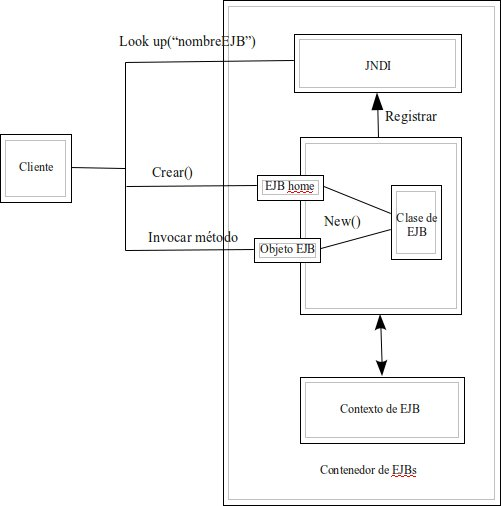
\includegraphics[width=0.5\textwidth]{./img/ejb.jpg}
\caption{Interacción entre el cliente y un componente EJB}
\end{center}
\end{figure}


\item CORBA \emph{Common Object Request Broken Architecture}: CORBA fue creado
por el \emph{Object Managemente Group}, su objetivo principal es permitir que
diferentes componentes escritos en diversos lenguajes y usando diferentes
plataformas se puedan comunicar entre si. Para especificar las interfaces de
los servicios se usa un lenguaje de definición de interfaces (IDL),

Los principales componente de CORBA son:
\item
\begin{enumerate}
  \item IDL: Lenguaje que especifica como los tipos de datos de CORBA deben
  ser utilizados en las implementaciones del cliente y del servidor, existen
  implementaciones del lenguaje para Ada, C, C++, Java, Pyton y Perl entre
  otros.
  
  
  \item \emph{Object Request Broker} (ORB): Es un contenedor de software que se
  encarga de localizar los objetos remotos, a tráves de este se comunican los
  diversos \emph{stubs} y \emph{skeletons}, y es el que ofrece la conectividad
  en un sistema CORBA.
  
  
  \item \emph{Stubs} y \emph{Skeletons}: Se usan para envolver o desenvolver
  invocaciones remotas de métodos en aplicaciones distribuidas  entre
  el cliente y el servidor. El skeleton es implementado por el servidor. Cuando
  se llama a un método remoto, la llamada al cliente pasa a través del stub
  
\end{enumerate}
En la figura 4.2 podemos ver como se comunican los componentes de CORBA.


\begin{figure}
\begin{center}
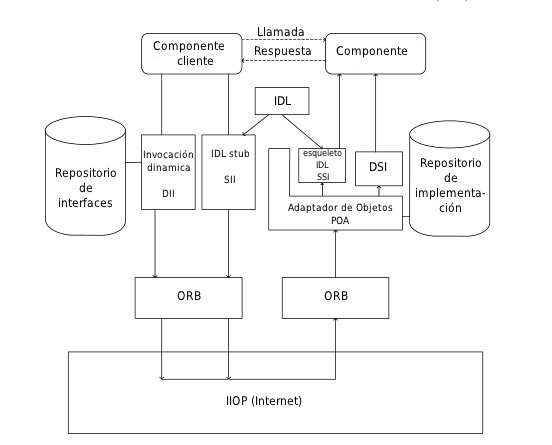
\includegraphics[width=0.75\textwidth]{./img/corba.jpg}
\caption{Infraestructura CORBA}
\end{center}
\end{figure}


\item OSGI (\emph{Open Service Gatewate Initiative}): Fue creado por un grupo
de compañías en tecnología incluidas Ericsson, IBM, SUN, Nokia, Intel, con el
fin de especificar, desarrollar y promover una plataforma de servicio libre,
para la administración de múltiples plataformas y servicios para todo tipo de
redes de dispositivos en hogares, vehículos, dispositivos móviles y otros
ambientes. OSGi provee de un ambiente común para componentes de servicios
llamados \emph{bundles}, los cuales son componentes que se integran
dinámicamente a un framework y proveen de diversos servicios. Los
servicios son los que ejecutan las tareas de negocio en OSGi, técnicamente, un
servicio es una interfaz de java, la cual evidentemente puede tener diversas
implementaciones. Los servicios son empaquetados junto con todos los recursos
necesarios para su ejecución, como imágenes, páginas HTML, etc. Un paquete de
servicio es es reusable, independiente y puede ser ejecutado de forma análoga
a como funcionan los dispositivos plug and play. Los servicios interactúan uno
con otro haciendo peticiones o proveyendo servicios en tiempo de ejecución, a
través de OSGi, las declaraciones de las conexiones en OSGi se tienen que
definir en un archivo de manifiesto.
OSGi provee los siguientes servicios:
\begin{enumerate}
  \item Manejar el ciclo de vida de los bundles.
  \item Resolver las interdependencias entre los bundles
  \item Mantener un registro de los servicios
  \item Disparar eventos y notificar a los \emph{listener} cuando el estado de
  un servicio sea modificado.
\end{enumerate}


\item Web Services: 
Web Service se puede definir de forma general como una aplicación o proceso
distribuido o virtual que permite conectar actividades o componentes de software
por medio de internet.
Existen diferentes frameworks para la creación de web services, a
continuación una pequeña descripción de los más populares.


\begin{enumerate}
  \item RPC-XML: Cuando internet y XML empezaron a hacerse populares, los desarrolladores se
  dieron cuenta de que era muy fácil enviar archivos a través de
  internet, haciendo uso de lo métodos de petición \gls{POST} o \gls{GET}, al
  principio cada desarrollador lo implementaba de la forma que le pareciera
  más conveniente, sin embargo pronto se dieron cuenta que era fácil construir
  un sistema \gls{RPC} usando tecnología y estándares existentes. Así nació
  RPC-XML, podría decirse que fue el primer \gls{framework}
  para servicios web. RPC-XML es una especificación un poco escueta e insegura,
  sin embargo en muy fácil de implementar y muy útil para pequeños fragmentos de
  información.
  
  \item SOAP: SOAP esta basado en RPC-XML, sin embargo es más robusto, y mas
  sofisticado que este, la transferencia de información la hace usando los
  protocolos SMTP y HTTP. SOAP provee de reglas para el manejo de
  procedimientos remotos usando XML. Con el fin de proveer una especificación
  para describir los métodos y los tipos de datos que se proveen por medio de
  una interfaz SOAP, se creo WSDL (\emph{Web Service Description Lenguage}).
  
  WDSL esta basado en XML  nos permite describir los requisitos de
  protocolo y  los formatos de los mensajes que permiten interactuar con los
  servicios web SOAP listados en su catálogo.
  
  \item REST \emph{Representational State Transfer}:  REST es un conjunto de
  restricciones arquitecturales para aplicaciones web, que intentan minimizar
  la latencia de las redes y al mismo tiempo maximizar la independencia y la
  escalabilidad de las implementaciones de los componentes.
  Las restricciones en las que se basa REST son las siguientes:
  \begin{enumerate}
    \item Separación de intereses(\emph{concerns}): Se deben separar
    los asuntos de las interfaces de usuarios con los asuntos del
    almacenamiento de datos.
    
    \item La comunicación debe de ser carente de estados (\emph{stateless}):
    Todas las peticiones del cliente deben de contener toda la información
    necesaria para entender la petición, los resultados no pueden variar debido
    a información contextual guardada en el servidor.
    
    \item Caché: Las respuestas a las peticiones deben de tener un identificador
    implícito o explicito que permita saber si la información debe de ser
    guardada en el caché o no.
    
    \item Debe de existir una interfaz uniforme entre los componentes, esto se
    logra agregando cuatro restricciones para las interfaces:
    identificación de recursos, manipulación de recursos a través de
    representaciones, mensajes auto descriptivos e hipermedia como motor de los
    estados de la aplicación.
    
    \item Estilos de sistema basado en capas: Permite que la arquitectura este
    compuesta por capas jerárquicas con las restricción de que cada componente
    solo puede ver la capa inmediata con la cual esta interactuando.
    
    \item Código bajo demanda (\emph{on demand}): Permite que la funcionalidad
    de los clientes pueda ser extendida por medio de la descarga y la ejecución
    de código como applets o scripts.

    
  \end{enumerate}
  

  
\end{enumerate}


\item Componentes de Android: La arquitectura de android facilita el reuso de
componentes de forma natural, de hecho las aplicaciones consisten en un
conjunto de componentes con un bajo acoplamiento, vinculados por medio de un
archivo de manifiesto, el cual describe  la forma en que los componentes
interactúan. Existen 6 tipos de componentes por medio de los cuales se
construyen las aplicaciones.
\begin{enumerate}
  \item Activities: Todas las vistas de una aplicación son componentes de tipo
  Activity. Las actividades usan vistas para formar las interfaces gráficas
  las cuales despliegan la información y responden ante eventos.
  \item Services: Los services se ejecutan sin que el usuario se de cuenta,
  son los encargados de actualizar las fuentes de los datos, de las
  actividades y de lanzar notificaciones, también sirven para ejecutar
  procesos aún cuando no existe ningún activity visible.
  \item Content Provider: Son los encargados de manejar y compartir las bases
  de datos, permiten compartir datos entre distintas aplicaciones.
  \item Intents: Son los encargados de pasar mensajes sencillos entre otros
  componentes, por medio de estos se pueden trasmitir mensajes a un gran
  número de Activities o Services.
  \item Broadcast Receivers: Son los encargados de estar al pendiente de los
  Intents, filtran los Intents y avisan a la aplicación cuando un intent con
  ciertas características es lanzado.
  
  \item Notifications: Permiten mandar notificaciones a los usuarios sin
  interrumpir al Activity que se este ejecutando.
  
\end{enumerate}

\end{itemize}

\section{Conclusión}
En el presente capítulo pudimos identificar las ventajas que se obtiene al
realizar una aplicación basada en componentes, la última sección  nos permitió
analizar las diferentes tecnologías usadas para el desarrollo de aplicaciones
basadas en componentes, gracias a esto podemos decir que la tecnología que mejor
se adapta al desarrollo del presente trabajo es servicios Web REST, se llegó a
esta conclusión debido a que es la única que cumple con todas las restricciones
definidas en los objetivos tales como, ocultar los detalles de configuración,
facilidad para reemplazar componentes, curva de aprendizaje baja, tecnología
emergente ampliamente usada y permite establecer comunicación de manera sencilla
entre el cliente y el servidor, en el capítulo 5 se definirá REST con mas
detalle.



\chapter{Marco de trabajo}
\section{OpenGL}

OpenGL es una especificación para desarrollo de software gráfico. La
sintaxis de OpenGL es simple y permite a los programadores desarrollar
aplicaciones gráficas complejas de una forma simple y lógica, además de permitir
a los fabricantes de tarjetas de videos crear características personalizadas.
OpenGL permite generar de forma dinámica los objetos y las operaciones
necesarias para la creación de aplicaciones tri-dimensionales interactivas.
OpenGL está diseñado para trabajar eficientemente incluso si la computadora que
despliega las gráficas no es la misma que la que está ejecutando el programa
gráfico y puede trabajar a través de la red incluso si el cliente y el servidor están en
diferentes computadoras, se diseñó para ser independiente del hardware, por
lo cual puede ser implementado en varias plataformas. La especificación de
OpenGL no incluye información sobre la creación de ventanas, ni para para
obtener datos de entrada del usuario, esto se hace de forma independiente. Las
imágenes y objetos son generados a partir de un pequeño conjunto de figuras
geométricas primitivas. OpenGL trabaja internamente como una máquina de
estados, una vez que se selecciona un estado este permanece hasta que se
modifique explícitamente.\\ Existen diversas bibliotecas libres que pueden
ampliar las funcionalidades de OpenGL entre las más usadas encontramos las siguientes: 
\begin{itemize}
  \item OpenGL Utility Library (GLU): contiene varia rutinas que usan los
  comando de bajo nivel de OpenGL para ejecutar tareas como poner matrices para
  la orientación y proyección de una vista especifica, ejecutar matrices y
  desplegar superficies.
  \item OpenGL Utility Toolkit (GLUT): Proporciona funciones de entrada/salida
  con el sistema operativo, así como administración de ventanas e interacción
  con estas por medio del teclado y el ratón.
  \item OpenGL Extensión para el sistema X Window (GLX): Provee una forma de
  crear un contexto de OpenGL y asociar a el una ventana sobre la cual se puede
  poner imágenes u objetos en maquinas que utilice el sistema X Windows.
\end{itemize}

La especificación JSR-231 define como implementar las funcionalidades de
OpenGL 2.0 en java así como la integración con AWT y Swing, gracias a ella
podemos hacer uso del procesador gráfico para la realización de aplicaciones en
java que haga uso de gráficos en 3D.

\subsection{OpenGL ES}
Existe un subconjunto de OpenGL optimizado para dispositivos móviles llamado
OpenGL ES,  el cual es el estándar para gráficos 3D en sistemas integrados,
los cual incluyen consolas, teléfonos y vehículos. \cite{kronos}
%OpenGL ES consiste en una serie de procedimientos y funciones que permiten a
%los programadores especificar los objetos y las operaciones necesarias para
%producir imágenes gráficas de alta calidad. \cite{kronosspec}

OpenGL ES está organizado en dos categorías OpenGL ES 1.x y OpenGL ES 2.x la
principal diferencia entre ambos es que 1.x utiliza 'fixed pipeline' y 2.X
utiliza un 'pipeline programable'.

%Existen dos especificaciones para usar OpenGL con java, la primera es 
La especificación JSR-239 el define como implementar las funcionalidades de
OpenGL ES en java.

Android incluye soporte para gráficas 3D de alto rendimiento por medio de
la API de OpenGL ES. Actualmente la especificación que soporta es similar a la
de J2ME JSR239.\cite{openglAnd} OpenGL ES 2  solo puede ser accedido usando
Android NDK (\emph{Native Development Kit}).

\subsection{WebGL}

WebGL se basa en OpenGL ES y permite crear aplicaciones que hagan uso del
procesador gráfico en aplicaciones web, la programación se hace por medio de
javascript, para esto es necesario el uso del elemento de HTML 5 HTMLCanvas,
dentro de este elemento dibujan las imágenes gráficas que van a ser
desplegadas programáticamente.

WebGL es soportado por Chrome, Firefox y Safari. La programación en páginas web
se hace por medio de javascript, la librería de Javascript vincula las funciones a OpenGL ES haciendo posible proveer contenido
3D acelerado por medio de hardware en una página web.

El principal problema con esta librería es que a pesar de ser poderosa es mas
lenta que las librerías en C++, aunque los nuevos compiladores just in
time han reducido significantemente esta brecha. \cite{1772933}

%Basado en lo anterior se decidió que el API que aporta una mayor
%flexibilidad y que se adapta mejor alas necesidades del presente documento es
%de Android para Open GL ES 1.

\subsection{Conclusión}

Basado en lo anterior y tomando en cuenta que en el presente trabajo el
despliegue de gráficas usando el GPU se hará en el cliente, el cuál es un
dispositivo móvil, se decidió que la versión que se usará para su desarrollo
será OpenGL ES 1.

%En el apéndice A se definen algunos conceptos básicos de programación que nos
%ayudarán a entender la forma como funciona OpenGL ES 1.



\section{ARtoolkit}

\subsection{Introducción}

ARToolkit es una biblioteca de código abierto, que facilita la
creación de aplicaciones de realidad aumentada, sus características principales
son las siguientes:

\begin{itemize}
 \item Es una plataforma simple para la creación de aplicaciones de realidad aumentada
en tiempo real.
\item  Multiplataforma.
\item Sobrepone objetos reales en marcadores virtuales.
\item Seguimiento rápido de marcadores con 6 grados de libertad en tiempo real.
\item Fácil rutina de calibración.
\item Biblioteca gráfica simple basada en GLUT.
\item Dibujado rápido de las imágenes basado en OpenGL.
\item Soporte de diversos lenguajes (Java, Matlab, C).
\item Código abierto con licencia GPL para uso no comercial.
\end{itemize} \cite{artkfl}

Las aplicaciones de realidad aumentada requieren de la identificación y
seguimiento de ciertos elementos, que después serán usados como base para
agregar elementos adicionales. ARToolkit cubre esta necesidad por medio de el
reconocimiento de marcadores predefinidos que se encuentren dentro del campo de
visión de una cámara de video, usando la forma y el tamaño de los marcadores, es
capaz de calcular la ubicación y la orientación de dichos marcadores, los
elementos adicionales se agregan haciendo uso de OpenGL.
\cite{Gaukrodger:2007:ARA:1328491.1328504}

La forma en como opera ArToolkit se explica en la figura 5.1.

\begin{figure}
\begin{center}
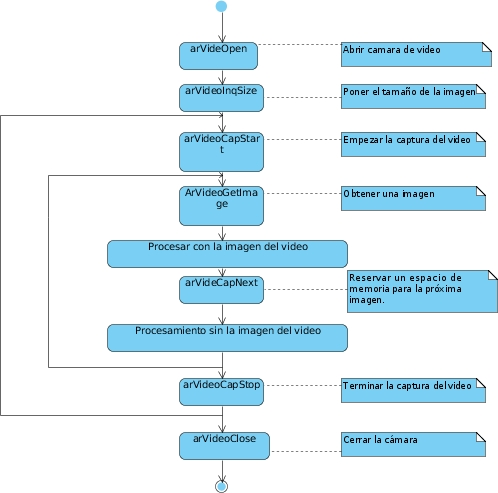
\includegraphics[width=0.7\textwidth]{./img/artoolkitDiag.jpg}
\caption{Diagrama de flujo de ARToolkit}
\end{center}
\end{figure}

\subsection{Implementaciones}

Existen diferentes implementaciones de ARToolkit como:
\begin{enumerate}
  \item ARToolKit for iOS: Permite utilizar las funciones de ARToolkit y
  provee clases en Objetive C que facilitan la programación. Funciona con
  iPhone 3G, iPhone 3Gs, iPhone 4, iPod touch 4G y iPad 2, la API es
  compatible con la App-Store de Apple. \cite{artoolkitios} 
  
  \item SLARToolkit: Basado en NyARToolkit y ARToolkit, nos provee de una
  librería para Silverlight y Windows Phone, puede ser usado con la API de la
  cámara web de Silverlight  o la clase de Windows Phone, PhotoCamera. Entre sus
  principales características esta: soporte incorporado para el API de
  aceleración 3D por hardware, detección de múltiples marcadores, uso de
  marcadores personalizados, desempeño adecuado para aplicaciones en tiempo real.
  \cite{slartoolkit}

  
  \item FLARToolkit: Basado en ARToolkit y NyARToolkit, permite la creación de
  aplicaciones de realidad aumentada usando Action Script 3 (en Flash). Permite
  el reconocimiento de marcadores, el cálculo de la orientación y posición, no
  incluye API para el dibujado de imágenes 3D, pero incluye clases para
  facilitar la integración con Papervision3D, Away3D, Sandy,
  Alternativa3D. \cite{flartoolkit}
 
  \item AndAR: AndAR es un proyecto basado en ARToolkit que permite la
  elaboración de aplicaciones de realidad aumentada en dispositivos móviles que cuenten con el
sistema operativo Android. AndAR contiene un API el cual es orientado a objetos
y completamente creado en java. El proyecto esta liberado bajo la licencia
pública general (GPL).
\cite{pandar}

Como se puede observar en la figura 5.2, se puede acceder a la cámara y obtener
la secuencia de video por medio del API en java, las imágenes se mandan a la
biblioteca de ARToolkit la cual esta escrita en C (android soporta C por medio
del kit de desarrollo nativo) , esta nos permite identificar el marcador y
calcular la matriz de transformación para el objeto 3D, a través de JNI
(\emph{Java Native Interface}) la matriz es mandada de nuevo a java, usando
OpenGL la matriz se aplica a las imágenes de la cámara generando los objetos 3D.\cite{aroasf}

\begin{figure}
\begin{center}
 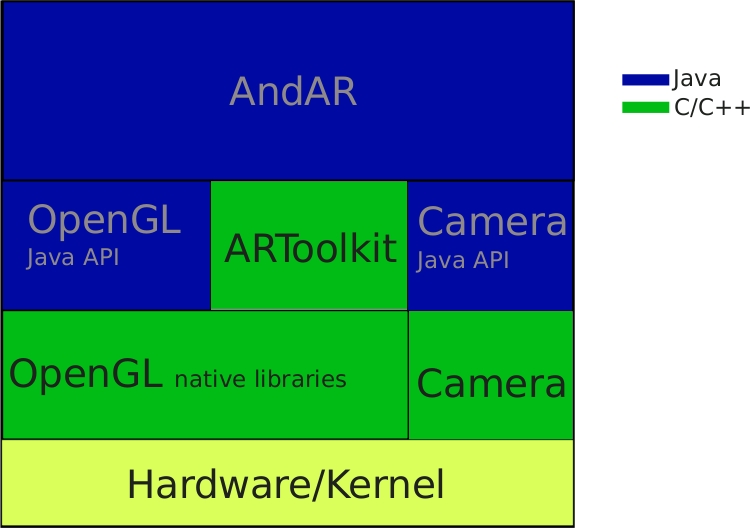
\includegraphics[width=0.5\textwidth]{./img/andAR.jpg}
\caption{Arquitectura de AndAR}
\end{center}
\end{figure}



\end{enumerate}

La implementación más adecuada para la realización del presente trabajo es
AndAr, esto debido a que es una librería para Android que permite usar todas las
características de ARToolkit, soporta marcadores múltiples, cuenta con licencia
open source, tiene una documentación adecuada y se encuentra optimizada para
trabajar sobre Android. %En el apéndice B podemos ver algunos de los detalles de
%la implementación y arquitectura de AndAr y como se integra con android.



\section{Android}

\subsection{Introducción}
Android es un sistema operativo con un ambiente de desarrollo abierto, esta
basado en el kernel de Linux.  Esta compuesto por varias partes incluidas las
siguientes:
\begin{itemize}
  \item Un sistema operativo basado en Linux, que provee interfaces de bajo
  nivel para comunicarse con el hardware, un administrador de memoria y un
  controlador de procesos, todos optimizados para dispositivos móviles.
  \item Librerías de código abierto para desarrollo de aplicaciones incluidos
  SQLite, WebKit y OpenGL.
  \item Una máquina virtual llamada Dalvik que permite la compilación en tiempo
  de ejecución.
  \item Un framework que expone los servicios a la capa de aplicación incluido
  un administrador de ventanas, un proveedor de contenidos, un administrador de
  ubicaciones, telefonía y servicios punto a punto.
  \item Un framework de interfaces de usuario usado para hospedar y lanzar
  aplicaciones.
  \item Un kit de desarrollo de software usado para crear aplicaciones.
\end{itemize}

Android permite acceder al hardware fácilmente por medio de varias APIs.

\newpage
Algunas de las características por las cuales se decidió usar android para la
realización del presente trabajo son las siguientes:
\begin{itemize}
  \item No se requieren de pago alguno para el licenciamiento, distribución o
  desarrollo.
  \item API para servicios basados en localización como GPS.
  \item Almacenamiento de datos compartidos.
  \item Gráficas optimizadas para móviles con aceleración por hardware; incluye
  una librería para gráficas 2D y soporte para gráficas 3D usando OpenGL ES.
  \item Librerías para reproducir y grabar audio y video.
  \item Un framework de aplicaciones que fomenta la reutilización de
  componentes.
\end{itemize}

Otra de las características de android es el soporte de aplicaciones corriendo
en segundo plano, estos nos permiten ejecutar acciones que realizan procesos
automáticos sin la intervención de los usuarios.

Android contiene una base de datos relacional, integrada, ligera, eficiente y
rápida basada en SQLite. 
%Por defecto una base de datos pertenece a una sola
%aplicación, pero si se desea, se puede modificar dicha característica.

\subsection{Arquitectura}

Android se compone de cinco capas (ver fig. 5.3):
\begin{enumerate}
  \item El Kernel de Linux, que contiene los servicios
esenciales, incluye los drivers, procesamiento y administración de memoria,
seguridad, y manejo de memoria.
\item Librerías esenciales: Escritas en C/C++ que incluye; librerías para audio
y video, las librerías gráficas OpenGL y SGL, soporte nativo para la base
de datos SQLite y WebKit para para el navegador web integrado.
\item Android Runtime: A pesar de que la sintaxis del lenguaje usado para
desarrollar sobre android es muy parecida a java, Dalvik no es una máquina
virtual de java, Android Runtime provee de la mayoría de las funcionalidades incluidas en una Java VM y además provee de
funcionalidades especificas de android. Dalvik es una máquina virtual optimizada
con el fin de asegurarse que un dispositivo pueda correr múltiples instancias
eficientemente.
\item Framework de aplicación: Provee de clases que se usan para crear
aplicaciones en android. También provee de abstracciones genéricas para acceso a
hardware y administra las interfaces de usuarios y los recursos de las
aplicaciones.
\item Capa de aplicación: Todas las aplicaciones, tanto las nativas como las de
terceros son construidas sobre la capa de aplicación.
\end{enumerate}
 
%En el apéndice C podremos encontrar algunos conceptos que nos permitirán
%entender mejor las diversas partes que componen android, como se relacionan
%entre si y los conceptos básicos desarrollar una aplicación por medio de estos.

\begin{figure}
\begin{center}
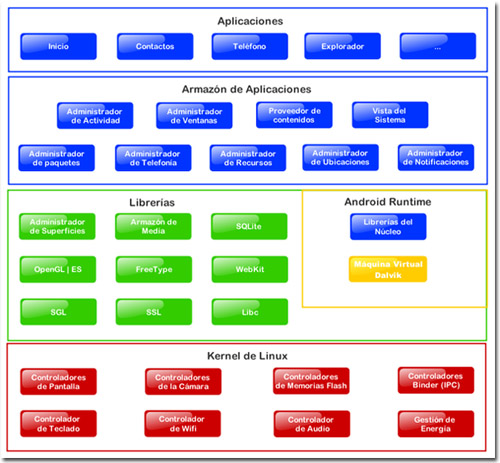
\includegraphics[width=0.85\textwidth]{./img/android-aplicaciones.jpg}
\caption{Arquitectura de Android}
\end{center}
\end{figure}



\section{Frameworks para el desarrollo rápido de aplicaciones}

\subsection{Spring Roo}

Spring roo es un marco de trabajo para desarrollo rápido de aplicaciones
usando Java, usa el principio de convención sobre configuración.

El desarrollo de aplicaciones en java requiere invertir una gran cantidad de
tiempo en la selección de tecnologías, configuración y realización de
actividades repetitivas que no son parte de los requerimientos funcionales,
Spring Roo permite tener listo este tipo de actividades en minutos, gracias a
esto es posible que los desarrolladores se enfoquen principalmente en la
lógicas del negocio lo que conlleva a una mayor productividad.
Está construido sobre tecnologías comúnmente usadas, lo que permite que los
desarrolladores utilicen sus conocimientos previos o en su defecto contar con
una gran cantidad de tutoriales disponibles.
Una de sus principales ventajas es que puede ejecutarse sobre cualquier ambiente
estándar para aplicaciones java, por lo que en caso de ya contar con uno
predefinido, puede usarse sin necesidad de configuraciones adicionales.

Spring Roo tiene como base dos tecnologías: AspectJ y Spring.

AspectJ permite generar diferentes miembros de la aplicación (métodos, campos,
etc) de forma independiente y tejerlos en tiempo de compilación, esto permite
a Spring Roo generar el código necesario para ejecutar ciertas tareas en un
archivo independiente sin revolverlo con la lógica de negocios implementada por
el desarrollador, y unirlos en tiempo de compilación,
de esta manera en tiempo de ejecución todo se ejecuta como un mismo
bloque. 

Spring es actualmente, el framework más popular para desarrollar aplicaciones
con java, Spring Roo permite utilizar no solo Spring Framework, sino también
otros componentes de Spring como Spring Security y Spring Web Flow.

Algunos otros componentes usados por Spring Roo son los siguientes:

\begin{itemize}
    \item   Adobe Flex: Utilizado en la creación de aplicaciones de internet
    enriquecidas.
    \item   Apache Maven: Permite generar descripciones proyectos y sus
    dependencias.
    \item   Apache Tiles: Herramienta para la generación dinámica de vistas. 
    \item   Hibernate: Facilita el mapeo objeto relacional entre tablas y
    objetos.
    \item   JSON: Como medio de envío de mensajes usando REST. 
    \item   Log4J:Librería para la impresión de mensajes con información sobre lo
  que esta sucediendo en la aplicación.
    \item   REST
    \item   Selenium: Permite la generación automática de pruebas.
\end{itemize}




\subsection{Grails}


El objetivo de Grails es la creación de un marco de desarrollo que contenga las
ventajas de Ruby on Rails y que al mismo tiempo aproveche las fortalezas de
un ambiente maduro como Java Enterprise. Grails esta construido sobre
tecnologías de código abierto, maduras, estables y ampliamente usadas como:
\begin{itemize}
  \item Groovy: Lenguaje orientado a objetos, ágil y de tipado dinámico.
  \item Hibernate: Estándar de facto para el mapeo objeto-relacional (ORM) en
  Java.
  \item Spring: Framework muy popular para desarrollo de aplicaciones java
  con soporte para Inversión de control.
  \item Quartz: Framework para la   calendarización de tareas.
  \item SiteMesh: Framework para creación de plantillas para aplicaciones web y
  decoradores para la creación de sitios con apariencia constante.
  \item Log4j
\end{itemize}


Grails crea una capa de abstracción adicional sobre las tecnologías antes
mencionadas con el fin de hacerlo más fácil de usar usando las ventajas que
proporciona Groovy como el tipado dinámico.

Grails permite usar las características de las tecnologías mencionadas por medio
de una interfaz simplificada, aunque también permite usarlos en su forma
original.



Grails sigue paradigmas como convención sobre configuración y no te repitas a ti
mismo, lo cual da como resultado un entorno de desarrollo estandarizado , eso
nos permite tener la configuración y los elementos básicos de una aplicación
lista en minutos por medio de algunas instrucciones simples que generan código
de forma automática.

Grails usa el patrón modelo-vista-controlador con el fin de separar la capa de
datos, las interfaces de usuarios y la lógica de control.

El flujo que sigue la aplicación a través de las capas es el siguiente: Un
usuario hace una petición por medio de un  navegador web, basados en la URL la
petición se delega a un controlador, el cual verifica si dicha petición es
válida y obtiene los datos necesarios haciendo peticiones a la capa de modelado,
una vez obtenida la información selecciona una vista y le pasa los datos
necesarios, la vista se encarga de desplegar la interfaz en el formato adecuado,
normalmente un GSP. Grails MVC esta basado en SpringMVC.

 GORM es una implementación de Grails que permite el mapeo objeto-relacional.
 Es decir, crea una relación entre las clases de dominio y las tablas de la base
 de datos. Está basado en Hibernate, un motor de ORM muy difundido en el ámbito de Java, con una capa
 Groovy por encima para simplificar su uso.

Las tecnologías más usada para la vistas de las aplicaciones en Grails son los
GSP(Groovy Server Page), están diseñado de forma muy similar a los JSP de java,
pero tratando de hacerlo más simple e intuitivo.

Grails hace un énfasis especial en las pruebas, nos provee de varios mecanismos
que facilitan la creación de diferentes tipos de pruebas, incluidas pruebas
unitarias, pruebas de integración y pruebas funcionales.


\subsection{Conclusión}
En esta sección vimos los dos frameworks para desarrollo rápido de aplicaciones
sobre la JVM (\emph{Java Virtual Machine}) más populares, ambos utilizan varias
tecnologías en común como base, principalmente Spring, esto con el fin de aprovechar los conocimientos
previos de los desarrolladores.
La principal diferencia entre ambos radica en el lenguaje base, mientras Roo
utiliza Java, Grail hace uso de Groovy.
Ambos frameworks se adaptan a las necesidades del presente trabajo, incluso se
desarrollo un prototipo con Roo que cumplía con las características deseadas,
sin embargo se decidió por Grails debido a lo fácil que resulta integrar plugins
de terceras personas.
Grails permite que mediante una sencilla instrucción como "grails install
plugin jaguarServer" se descarguen todas las clases, vistas y librerías que nos
permitan tener una aplicación 100\% funcional y que permita hacer las
modificaciones pertinentes si así se desea.


\section{Groovy}
Groovy es un lenguaje de programación ágil y dinámico
de propósito general para la máquina virtual de Java (JVM) creado en el
2003. Uno de los objetivos de su creación fue tener un lenguaje que aprovechara
las fortalezas de Java, agregarles ciertas características similares a Ruby y
Pyton y que al mismo tiempo fuera fácil de integrar con la plataforma java.

Groovy comparte muchas características con java, por ejemplo el modelo de
objetos, hilos y de seguridad además de poder integrarse con las clases y
bibliotecas existentes, pero también agrega características de lenguajes
más ágiles como closures, builders y tipado dinámico.
Otras ventajas que permiten acortar los tiempos de desarrollo son:
El manejo automático de dependencias y las configuraciones, con el
objetivo de que el desarrollador se enfoque solamente en el código,
la inclusión un servidor embebido, útil sobre todo en la fase de pruebas, el
reflejo automático en la aplicación de los cambios en en código, sin la
necesidad de reiniciar el servidor. También nos ofrece un scaffolding lo que nos
permite la lectura, escritura, actualización y borrado de datos de forma automática.
Además de que es muy fácil agregar más características implementadas por
terceros por medio de plugins.

Al compilar código Groovy se genera bytecode, el cual es casi indistinguible del
generado por java, por lo cual lo podemos usar en cualquier parte en donde se
pueda usar java.



Actualmente por medio del JSR 241 \cite{jsr241} se está trabajando en su
estandarización para su posible inclusión como componente oficial de java.

Algunas de las características de sintaxis que comparten Java y Groovy son:
\begin{itemize}
  \item Palabras reservadas o sentencias
  \item Manejo de excepciones
  \item Definiciones de clases, interfaces, métodos y campos.
  \item Instanciación de objetos.
  \item Empaquetamientos e importaciones.
  \item Operadores, expresiones y asignadores.
  \item Estructuras de control.
  \item Comentarios.
  \item Lenguaje compilado.
\end{itemize}

La principal diferencia entre Groovy y otros lenguajes de su tipo como Ruby
o Phyton es que es un lenguaje compilado, esto con el fin de hacerlo
completamente compatible con java, todas las clases de Groovy son convertidas a
bytecode por medio del compilador de Groovy y luego son ejecutadas.

Algunas de las características disponibles en Groovy que no son parte de java
son:

\begin{itemize}
  \item Closures.
  \item Soporte de métodos avanzados sobre cadenas de caracteres.
  \item Operadores sobrecargados y estructuras sintácticas que permiten acceder
  a las clases de java existentes.
  \item Mejoras en la sintaxis de los tipos de de datos existentes y nuevos tipos
  de datos.
 % \item An extended library of methods onto existing Java classes
 \item Permite ser escrito en forma de script (se crea una clase ejecutable de
 forma automática)
\end{itemize}


\section{Rest}

REST significa  Transferencia de Estado Representacional (por sus siglas en
ingles), el concepto fue introducido por primera vez en el año 2000 en la
disertación doctoral de Roy Fielding. Como comentábamos anteriormente REST no es
una arquitectura en sí misma, sino un conjunto de reglas de diseño para
sistemas hipermedia distribuidos que define los roles y las características  de
los componentes y conectores que deben ser usados para crear un sistema.
REST hace uso de diversos estándares como HTTP, URL, XML, HTML, JPEG, tipos de
MIME, etc.

REST ignora los detalles de la implementación de los componentes y la sintaxis
de los protocolos y se enfoca en los roles de los componentes, las restricciones
de interacción con otros componentes y la interpretación de datos
significativos. Los componentes de REST se comunican por medio de transferencias
de representaciones de los datos en algún formato estándar.

Se usa normalmente el nombre RESTful para identificar a los sistemas que cumplen
con las reglas definidas por REST.

En el capítulo 5 ya se menciono cuales son las características que deben debe
tener un sistema para que, a continuación explicaremos la razón de dichas
restricciones.



\begin{itemize}

 \item Separación de intereses: Al separar las interfaces de
 usuarios de los datos se mejora la portabilidad de las interfaces de usuario a
 través de diferentes plataformas, también se logra mejorar la escalabilidad al
 simplificar los componentes del servidor. Esta separación también nos permite
 que los componentes funcionen de forma independiente.
 
 \item  La comunicación carente de estados: Gracias a esto se mejora la
 visibilidad, fiabilidad y escalabilidad de los componentes. La visibilidad
 debido a que los mensajes son auto-descriptivos y contienen toda la información
 necesarias, gracias a esto solo son necesarios los datos de una petición para
 obtener obtener el comportamiento adecuado. Fiabilidad, si la petición no tiene efectos secundarios, se puede enviar repetidamente hasta obtener una
 conformación, en caso de que si los tenga podemos hacer lo mismo, pero cuando
 el servidor recibe la misma petición dos veces, la segunda vez solo envía el
 mensaje de confirmación sin ejecutar la acción. La escalabilidad se logra
 gracias a que al no existir estados en el servidor, se pueden liberar
 rápidamente los recursos. También nos permite procesar varias peticiones en
 paralelo sin preocuparnos de como se afectan las peticiones entre ellas.
 Las desventajas de la carencia de estados es que reduce el rendimiento debido
 la obtención de datos repetidos, aunque el uso del caché mejora este aspecto.


    
    \item Caché: Si cierta petición permite el uso de caché, entonces todas
    las peticiones equivalentes obtendrán el mismo resultado, esto nos permite
    eliminar algunas interacciones mejorando la eficiencia, la escalabilidad y
    reduciendo los tiempos de latencia, la desventaja principal es que el
    usuario puede obtener datos que fueron exactos en algún momento anterior,
    pero que ya no lo son al momento de la petición.
    
    
    \item Interfaz uniforme entre los componentes: Esto simplifica la
    arquitectura general y mejora la visibilidad de las interacciones, las
    interfaces son independientes de los servicios que presta la aplicación y la
    información se transfiere de forma estandarizada, como habíamos
    mencionado existen cuatro restricciones para las interfaces:
        \begin{itemize}
            \item Identificación de recursos: Los recursos son identificados de
            forma individual en una petición, por ejemplo el servidor no manda
            todos los datos de una tabla, en vez de eso los filtra y manda una
            representación de ellos por medio de un archivo HTML, XML o JSON.
            \item Manipulación de recursos a través de representaciones: Cuando
            un cliente obtiene un recurso, puede modificarlos o eliminarlos del
            servidor, suponiendo que tiene los permisos correspondientes.
            \item Mensajes auto descriptivos: Cada petición incluye toda la
            información necesaria para describir el proceso que se tiene que
            ejecutar.
            \item Hipermedia como motor de los estados de la aplicación: La
            única forma para que un cliente pase de un estado de la aplicación a
            otra es por medio de ligas que son procesadas por el servidor y que
            permite ejecutar ciertas acciones.
        \end{itemize}    
      
   
    \item Estilos de sistema basado en capas: Al restringir el conocimiento del
    sistema a una sola capa se pone un límite a la complejidad general del
    sistema y promueve la independencia de los componentes. Las capas también
    permiten encapsular ciertos servicios y protegerlos de usuarios que no
    tengan los permisos para ejecutarlos. Una ventaja adicional es que facilita
    el balanceo de cargas entre múltiples servidores.
    
    \item Código bajo demanda: Esto permite acceder a recursos sin saber a
    priori como procesarlos, el cliente es el encargado de procesar los recursos
    de forma automática, esto mejora la
    extensibilidad, la configurabilidad e incluso la eficiencia y el rendimiento, debido que este recurso interactúa
    con el cliente de forma local.

\end{itemize}

\newpage
Los elementos que debe contener una arquitectura basada en REST son los
siguientes:

\begin{enumerate}
  \item Datos: REST se comunica por medio de representaciones de datos en un
  formato que se encuentre dentro de un conjunto de formatos estándares,
  este es seleccionado dinámicamente basandose en la naturaleza de los datos.
  \begin{enumerate}
    \item Recursos: Cualquier información que pueda ser nombrada
    \item Representaciones:Una representación de un recurso en un momento
    dado, consiste en datos, meta-datos describiendo los datos e incluso
    meta-meta datos describiendo meta-datos.
  \end{enumerate}
  \item Conectores: Proveen de interfaces que permiten la comunicación entre
  componentes y al mismo tiempo esconden los detalles de implementación de los
  recursos y los mecanismos de comunicación. Los principales conectores son el
  servidor y el cliente.
\end{enumerate}

\subsection{REST y Grails}

La mayoría de las implementaciones de REST para la WWW se basan en los mismos
estándares de facto, en esta sección veremos el caso específico de la
implementación de REST para Grails, aunque la mayoría de los conceptos son
válidos para cualquier marco de trabajo que se comunique a través de internet.

La separación de intereses se logra mediante el protocolo HTTP que nos permite
tener en un servidor los datos, pueden accesarse mediante peticiones y en los
clientes las interfaces de usuarios.
La comunicación carente de estados podemos lograrla mediante peticiones que
contengan toda la información necesaria, para lograr esto se usan patrones de
URLs y métodos de HTTP para representar las diferentes acciones.
El caché se puede hacer del lado del cliente mediante la meta etiqueta de HTML
CACHE-CONTROL o de lado del servidor con ayuda de diferentes librerías como
ehcache.
Para la interfaz uniforme se logra mediante HTTP el cual permite el acceso a
recursos basados en URIs, métodos. códigos de estados, cabeceras y contenidos
definidos por el tipo de MIME.
La restricción de código bajo demanda es cubierta por medio de applets y
Javascript.


Las implementaciones de REST para aplicaciones web se basan en:
\begin{itemize}
  \item Archivos planos con formato XML o JSON como medio de trasmisión de
  datos.
  \item Patrones de URL que sirven para representan al sistema.
  \item Métodos de HTTP que representan a las operaciones básicas de  asociadas
  a una base de datos.
\end{itemize}

Cada método de HTTP es mapeado a una acción de la aplicación y a su vez con un
evento de la base de datos como se muestra en la siguiente tabla.

\singlespacing
\begin{center}
\begin{tabular}{|p{3.5cm}|p{6.5cm}|p{3.5cm}|}
\hline
\textbf{Método} & \textbf{Acción} & \textbf{Función de base de datos} \\
\hline
GET & Obtención de datos & SELECT\\
PUT & Actualización de datos & UPDATE\\
POST & Guardar datos & INSERT\\
DELETE & Eliminar datos & DELETE\\
\hline
\end{tabular}
\end{center}
%\doublespacing



\section{Json}
El formato clásico para transmisión de representaciones de objetos por medio de
HTTP es XML, este formato es altamente extendido y tiene soporte para casi todos
los lenguajes de programación. XML fue creado originalmente para que sea legible
por humanos, sin embargo a medida de que los archivos se van haciendo mas
grandes, cada vez es más difícil la lectura intuitiva de estos, otro inconveniente es que
requiere de una gran cantidad de meta-información, para mandar un valor se
requieren de dos etiquetas, más las etiquetas padres, etc. Toda esta información
extra ralentiza la transmisión de información entre un cliente y un servidor, y
hace que el proceso de creación de un archivo requiera de una gran cantidad de
memoria.
Un formato que permite eliminar estas desventajas es JSON, un archivo
JSON es más compacto que un XML y permite la creación y lectura de archivos de
forma eficiente, otra ventaja es que no se necesitan librerías adicionales en
el cliente para leer la información y tampoco hay que preocuparse por el
funcionamiento adecuado entre múltiples navegadores, ya que cualquier
navegador que soporte Javascript soporta JSON, debido a que este es un
subconjunto de la notación de objetos de Javascript.

Los objetos JSON están construidos por dos estructuras soportadas en la mayoría
de los lenguajes de programación: mapas y listas, los cuales pueden estar
anidados. La sintaxis es muy simple, se utilizan llaves(\{\}) para definir los
limites de los elementos, dos puntos (:) para separar entre una propiedad y su
valor y los elementos de una lista se posicionan entre corchetes ($[]$), los
valores se separan por comas.

Se soportan los siguientes tipos de datos para valores.
\begin{itemize}
  \item Cadenas de caracteres.
  \item Números.
  \item Otros objetos JSON.
  \item Caracteres.
  \item Valores nulos(representados por la cadena de caracteres null)
  \item Booleanos.
\end{itemize}



\begin{verbatim}
{"objeto3D": {
   "id": "xyz",
   "nombre": "android.obj",
   "mtl": "android.mtl",
   "textura": "android.jpg",
   "": {
     "marcadores": [
       {"nombre": "hiro.patt", "ubicacion": "/texturas/uno", 
            "tamano":"300"},
       {"nombre": "android.patt", "ubicacion": "/texturas/dos", 
            "tamano":"500"}
     ]
   }
 }}
 
    Código 5.1: Ejemplo de archivo JSON.
\end{verbatim}


\section{Conclusión}
Durante este capítulo se definieron las tecnologías que se usarán durante el
desarrollo del presente trabajo.
Se usará OpenGL ES para el despliegue de los gráficos debido a que es el
estándar para aplicaciones gráficas sobre dispositivos móviles.
AndAR para aplicaciones de realidad aumentada, debido a que implementa todas las
características de ARToolkit y contiene una documentación adecuada, además de
ser compatible con los demás elementos usados.
Android por ser un sistema operativo de código abierto, ampliamente usado e
implementado en diversos teléfonos inteligentes, la mayoría de los cuales
cuentan con los artefactos necesarios para lograr una exitosa implementación de
aplicaciones de realidad aumentada.
Grails por ser un marco de trabajo para la creación rápida de aplicaciones,
basado en tecnologías abiertas ampliamente usadas.
Groovy como lenguaje de lado del servidor por ser el lenguaje dinámico más usado
que corre sobre la JVM y por tener una curva de aprendizaje muy baja para los
desarrolladores de Java.
REST para comunicación entre componentes debido a que es ampliamente usado y
permite esconder los detalles de implementación y enfocarse en la comunicación
entre los diversos componentes.
Y finalmente JSON por permitir la fácil serialización y deserialización para su
envío a través de HTTP sin agregar etiquetas que podrían hacer más pesados los
objetos y más lento su envío.









\chapter{Caching basado en geoposicionamiento}

\section{Introducción}


La adquisición, inicialización y liberación repetitiva de objetos
usualmente requiere de una gran cantidad de recursos, esto puede llegar a
convertirse en un cuello de botella. La forma común de solucionar este problema
es haciendo uso de un sistema de caché, este permite mejorar el
rendimiento debido a que evita generar los mismos procesos de forma
reiterada.

El patrón caching describe como evitar la generación duplicada de recursos, esto
se logra manteniendo los recursos por un tiempo después de generados.


Existen dos procesos esenciales al momento de generar un sistema de caching, el
primero es la obtención del recurso, este se puede hacer de diversas formas
entre ellas:
\begin{itemize}
  \item Preparadas: Se usa cuando al menos parte de los recursos que se
  utilizarán pueden ser predichos, permite generar los recursos antes de que
  sean solicitados.
  \item Bajo Demanda: Se usa cuando los recursos no pueden ser predichos, los
  recursos se generan la primera vez que son solicitados.
\end{itemize}
El segundo proceso esencial es la liberación de recursos, existen diversos
algoritmos que permiten hacer esto, entre los más populares tenemos:
\begin{itemize}
  \item Menos recientemente usado (MRU): Descarta los elementos que llevan más
  tiempo sin ser usados.
  \item Menos frecuentemente usado (MFU): Descarta los elementos que se han
  usado menos veces.
\end{itemize}


Diversas implementaciones de caching para numerosos lenguajes han sido
creadas, las técnicas que implementan
funcionan adecuadamente en entornos tradicionales, sin embargo, el tener
servicios basados en localización (SBL) permite obtener información adicional
que puede ser usada para mejorar los algoritmos de caching, especialmente los usados
en la predicción de recursos y en la liberación de los mismos, esto nos permiten
ofrecer características personalizadas a los usuarios. Esto es lo que nos
motivo a crear una implementación de un sistema de caching, que permita predecir
y eliminar recursos dependiendo de la ubicación de estos y de los usuarios.


Los algoritmos MRU y MFU son una forma eficaz de eliminar recursos cuando no
se cuenta con información adicional sobre estos, sin embargo, el
asociar los recursos a una localización y el tener conocimiento de la ubicación
geográfica de los usuarios, permite crear un algoritmo más eficiente. 

El
algoritmo de liberación de recursos basado en localización al que llamaremos
"Mas distante del usuario" (MDU) se basa en el hecho de que entre más cerca este
un usuario de un objeto las probabilidades de que ese objeto sea usado son
mayores, conforme se va alejando del objeto las probabilidades disminuyen, esto
permite deducir que los objetos que deben ser eliminados cuando sea necesario
son los que se contienen coordenadas más alejadas de los usuarios.
Un algoritmo similar se utilizará para la predicción de recursos usados por
sistemas de caching preparados.

\section{Caching}



Un sistema de caching permite guardar temporalmente recursos que han sido
generados previamente, estos se pueden obtener posteriormente mediante un
identificador como puede ser un puntero, una referencia o una llave
primaria,evitando así generarlos nuevamente, cuando el sistema considera que el
recurso no será utilizado nuevamente, o cuando se requiere de espacio para
almacenar recursos que tienen más probabilidades de usarse, estos se liberan,
una vez liberados es necesario volver a generarlos para usarlos de nuevo.

Para implementar el patrón caching es necesario seguir los siguientes pasos:

\begin{enumerate} 
  \item Seleccionar el recurso: Seleccionar que elementos van a ser almacenados,
  normalmente se selecciona los que tiene muchas probabilidades de ser usados
  frecuentemente y su generación y/o obtención es costosa.
  \item Determinar una de caching: Dicha interfaz debe contener un método para
  agregar elementos al caché y otro para liberarlos.
 \item Crear una implementación de la interfaz: Implementar los métodos para
 agregar y eliminar elementos de forma eficiente.
 \item Implementar una estrategia de liberación de recursos: El almacenamiento
 temporal de elementos requiere de memoria, la cual es limitada, por eso es
 importante liberar recursos que tengan pocas posibilidades de volver a
 usarse.
\end{enumerate}


El caching agrega una capa de indirección adicional, lo que hace que el proceso
sea más complejo, sin embargo las ventajas son mayores, debido principalmente a
que los recursos se adquieren rápidamente, entre las principales ventajas de implementar
el patrón caching están las siguientes:

\begin{itemize}
  \item Rendimientos: Se puede acceder rápidamente a los recursos frecuentemente
  usados.
  \item Escalabilidad: Evita que el mismo recurso sea adquiera y se libere en
  múltiples ocasiones.
  \item Complejidad en el uso: El implementar un sistema de caching es un
  proceso sencillo y una vez implementado es transparente para el usuario.
\end{itemize}


El implementar un sistema de caching ocasiona un incremento en el uso de la
memoria, por lo cual es necesario establecer un balance óptimo
entre la cantidad de memoria usada y el rendimiento, si se guardan demasiados
recursos, los beneficios de implementar un sistema de este tipo disminuirán
drásticamente.

%En el presente trabajo se implementa un sistema de caching que permite
%maximizar

Cuando se tiene un sistema en tiempo real, el tiempo utilizado en la creación ,
obtención y liberación de objetos se vuelve especialmente crítico, sobre todo
por que es tiempo en que el usuario permanece esperando.


%2s
\section{Implementación}



Para el presente trabajo se realizó una implementación de un sistema de
caching basado en localización, el objetivo es minimizar la creación de objetos
bajo demanda, inferir que objetos van a ser usados y crearlos de forma asíncrona
antes de que sean pedidos, esto con el fin de disminuir los tiempos de espera de
los usuarios. 


En la figura 6.1 se
muestra un diagrama de actividades que describe el algoritmo que se usará el en
la implementación del sistema de caching. La figura 6.4 muestra el ciclo de
vida de los objetos que se generan al momento implementar el algoritmo de
caching con cacheo preparado, incluyendo la generación, obtención y eliminación
de los objetos cacheables.  La liberación de recursos se realiza en un proceso
independiente y el desarrollador podrá escoger entre tres algoritmos diferentes:
MRU, MFU y MDU. (Ver fig. 6.2)

\begin{figure}
\begin{center}
 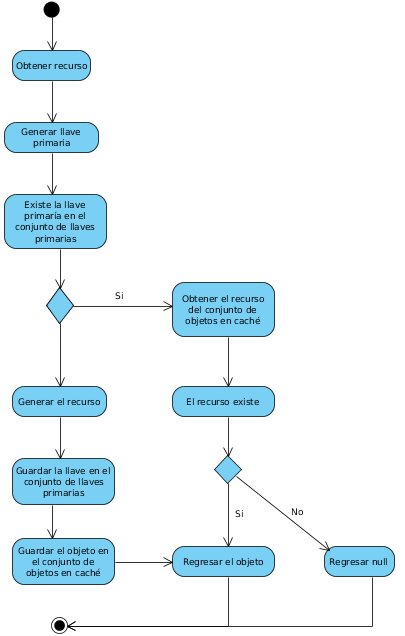
\includegraphics[width=0.55\textwidth]{./img/caching4.jpg}
\caption{Diagrama de actividades del algoritmo de caching}
\end{center}
\end{figure}

En la figura 6.3 se pueden observar las clases principales que intervienen en la
generación de objetos de caching, dichas clases se describen a continuación.

\begin{itemize}
  \item CacheKeys: Almacena identificadores únicos hacia los objetos contenidos
  dentro del objeto caché.
  \item CacheObjects: Almacena los objetos cacheados.
  \item BaseDisposal: Clase base para la liberación de objetos, permite eliminar
  los objetos que tienen pocas probabilidades de ser usados, estos se
  seleccionan de acuerdo con el algoritmo de liberación seleccionado.
  \item PrimeCaching: Permite generar objetos con alta probabilidad de
  ser usados antes de que el usuario los requiera.
  \item BaseCaching: Permite generar los objetos la primera vez que se
  solicitan.
  \item BaseCaching: Contiene todos los elementos necesarios para generar,
  obtener y liberar objetos almacenados en el caché.
\end{itemize}

Cualquier implementación de un sistema de Caching deberá extender la clase
BaseCaching, en este trabajo se harán dos implementaciones, caching bajo demanda
y caching preparado.

La implementación se basa en el paradigma de convención sobre configuración,
para que un objeto sea guardado en un caché solo es necesario agregar la
anotación @Cached con el atributo type describiendo el tipo de caché que se va
a implementar, como se muestra en el siguiente ejemplo:

\begin{verbatim}
    @Cached(type="NumbersCachingImp")
    public Object cachedObject;
\end{verbatim}

El framework inyecta automáticamente la funcionalidad en tiempo de compilación,
esto es posible gracias a que se hace uso de AspectJ. AspectJ es una extensión
que permite implementar el paradigma de programación orientada a aspectos en
java, dicho paradigma permite encapsular de forma independiente las
funcionalidades que se diseminan a través de todo el sistema en una unidad de
modularización llamada aspecto, los aspectos se combinan con las clases en
puntos de enlace definidos por el desarrollador. En este trabajo se hace uso de anotaciones para
definir los puntos de enlace.

Con el fin de seguir el paradigma de convención sobre configuración se han
definido una serie de reglas que permiten la implementación de clases de caching
sin necesidad de configuraciones adicionales.

Las reglas para definir el algoritmo de caching son las siguientes:

\begin{itemize}
  \item Todos los caching deben de estar en el paquete
  *.caching.implementations.
  \item Deben de extender a BaseCaching o una de sus subclases.
  \item El nombre de la clase debe de terminar con CachingImp. 
  \item Debe sobreescribir correctamente los métodos solicitados.
  \item Sobre la clase config se debe de usar la anotación  @Disposal, la cual puede
contener los atributos algunos, todos o ninguno de los siguientes atributos:
    \begin{itemize}
        \item disposalEnum : Indicando la estrategia que va a ser usada para
        eliminar elementos de memoria cuando sea requerido, por defecto la estrategia
        usada será MFU.
        \item maxObjects: Indicando el número máximo de objetos, por defecto será de
        100.
        \item maxMeters: Usado solamente si se utiliza un algoritmo de
        liberación de memoria basado en localización, indica el número de metros máximos entre
        el usuario y los elementos existentes en memoria para garantizar que
        estos últimos no sean eliminados, el valor por defecto es 1000.
        \item preloadAsync: Usado solamente si se tiene un sistema de caching bajo
        demanda, el valor booleano indica si los elementos que se predicen
        pueden ser usados y se generan de forma síncrona o asíncrona, el valor
        por defecto es falso.         
    \end{itemize}
\end{itemize}
      
        
 También es posible implementar algoritmos para liberación de
 recursos personalizados siguiendo estas simples reglas:
 \begin{itemize}
   \item Posicionar la clase en el paquete *.caching.disposal
   \item Deben de terminar con la palabra disposal.
   \item Modificar las clases Disposal Factory y DisposalEnum para agregar la
   nueva implementación.
   \item Implementar la interfaz BaseDisposal.
 \end{itemize}



\begin{sidewaysfigure}
\begin{center}
 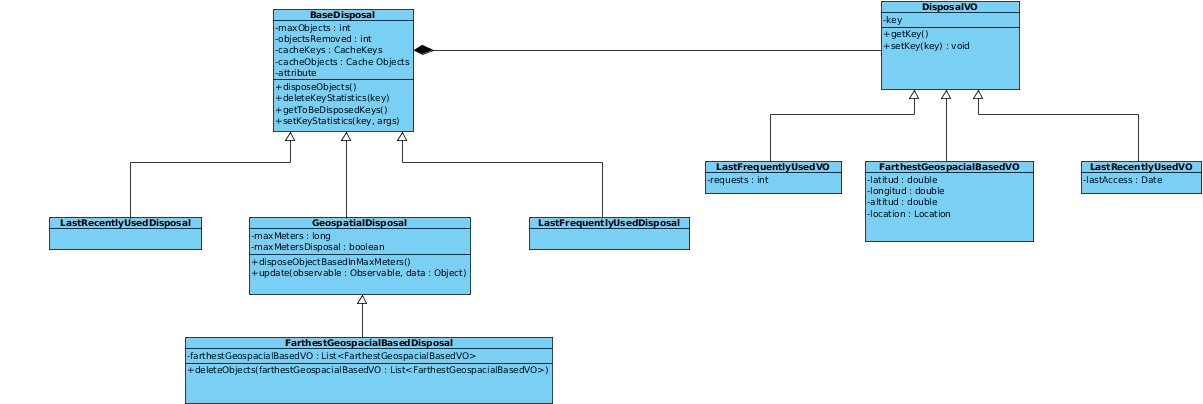
\includegraphics[width=1\textwidth]{./img/caching1.jpg}
\caption{Diagrama de clases de la implementación de Caching}
\end{center}
\end{sidewaysfigure}

\begin{figure}[ht]
\begin{center}
 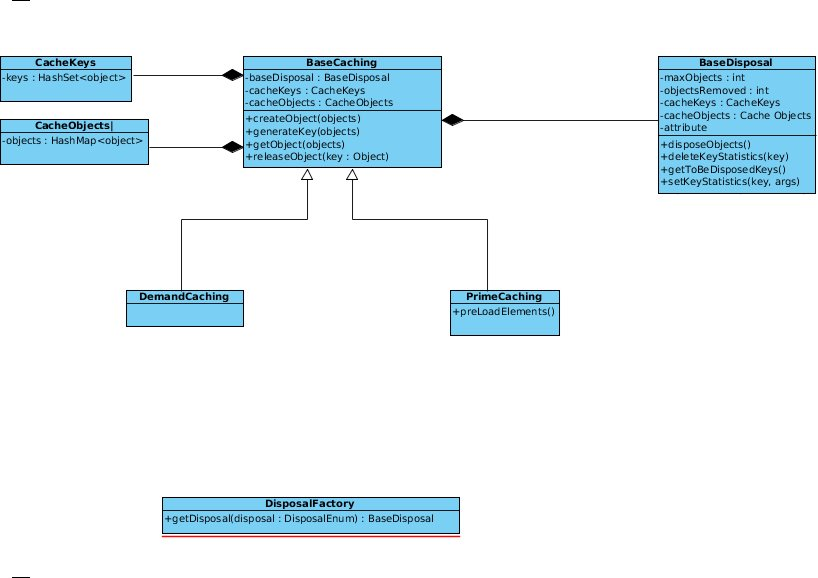
\includegraphics[width=0.9\textwidth]{./img/caching2.jpg}
\caption{Diagrama de clases de metodología de liberación de recursos}
\end{center}
\end{figure}



\begin{figure}[ht]
\begin{center}
 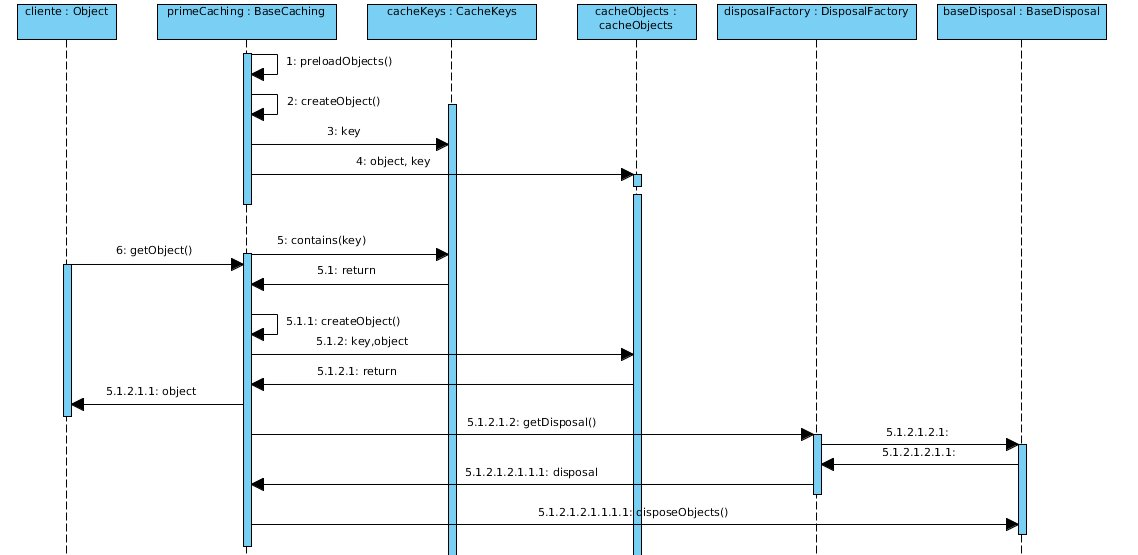
\includegraphics[width=0.9\textwidth]{./img/caching3.jpg}
\caption{Diagrama de secuencia del módulo de caching}
\end{center}
\end{figure}

\section{Conclusión}
En el presente capítulo se describió una implementación de un sistema de caching
para dispositivos móviles, se implementaron las características generales de la
mayoría de los sistemas de caching actuales. El valor agregado sobre los sistema
en el mercado, es que permite la obtención y liberación de recursos basandonos
en la localización del usuario y meta-información relativa a la localización
geográfica de los objetos cacheables.




%\chapter{Desarrollo rápido de aplicaciones}
%\section{Convención sobre configuración}



\chapter{Arquitectura propuesta}

\section{Introducción}
En este capítulo se explica la arquitectura basada en componentes para el
desarrolló rápido de aplicaciones de realidad aumentada propuesta, también se
describen los componentes que la integran y las reglas necesarias para su
implementación.

La Arquitectura para desarrollo de aplicaciones de realidad aumentada
(ADARA), pretende proporcionar una metodología y un marco de trabajo que permita
el desarrollo rápido de aplicaciones de realidad aumentada haciendo uso de un
entorno de desarrollo estandarizado y que permita modificar o reemplazar sus
componentes de forma independiente.

ADARA es una arquitectura cliente servidor basada en los paradigmas de
convención sobre configuración y programación orientada a componentes, esta
liberada bajo la licencia GPL.

Dividir la aplicación por componente permite utilizarlos de forma independiente,
integrarlos en otros sistemas o reemplazarlos fácilmente. 
Utilizar el principio de convención sobre configuración permite reducir los
tiempos de desarrollo debido a que el programador se enfoca en cumplir los
requisitos funcionales, sin preocuparse por la configuración o la separación de
intereses.


\section{ADARA}

ADARA esta compuesta por dos subsistemas uno para el cliente y otro para el
servidor, los cuales a su vez contienen diversos componentes.

El subsistema cliente es el que ejecuta funcionalidades de realidad
aumentada como desplegar objetos 3D y desplegar menús con información por medio
del procesador gráfico. Puede ser visto como una capa de abstracción sobre
Android la cual permite agilizar el desarrollo de aplicaciones de realidad
aumentada.

El subsistema servidor permite la administración de usuarios, información,
aplicaciones, empresas, generación de reportes y análisis de las acciones de
los usuarios, también provee una interfaz que permite la sincronización de datos
por medio de servicios Web REST. Puede ser visto como una capa de
abstracción sobre grails que permite la administración de aplicaciones de
realidad aumentada que usen ADARA cliente.


La comunicación entre los componentes de ADARA servidor y
ADARA cliente se hace por medio de servicios Web REST.

ADARA crea por defecto todos los elementos necesarios para usar una aplicación
de realidad aumentada, si se desea, sólo es necesario desplegar ADARA Servidor
en un servidor web  y ADARA Cliente en un dispositivo móvil con el sistema
operativo Android para contar con una aplicación completamente funcional.

En la figura 7.2 podemos ver el diagrama de casos de uso del servidor y en la
figura 7.1 el diagrama de casos de uso del cliente, cada caso de uso se
convierte en un componente, esto con el fin de poder modificarlos o
reemplazarlos de forma independiente.

\begin{figure}[ht]
\begin{center}
 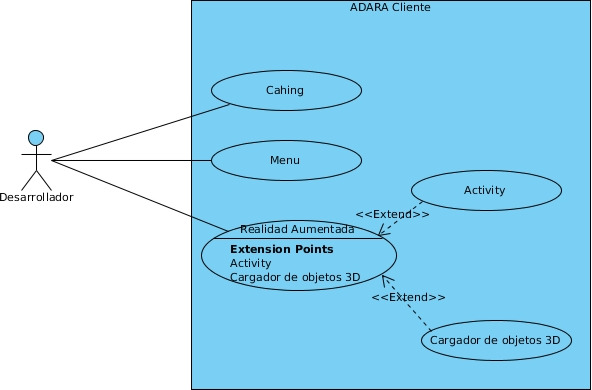
\includegraphics[width=0.75\textwidth]{./img/CUCliente.jpg}
\caption{ADARA Cliente}
\end{center}
\end{figure}

\begin{figure}[ht]
\begin{center}
 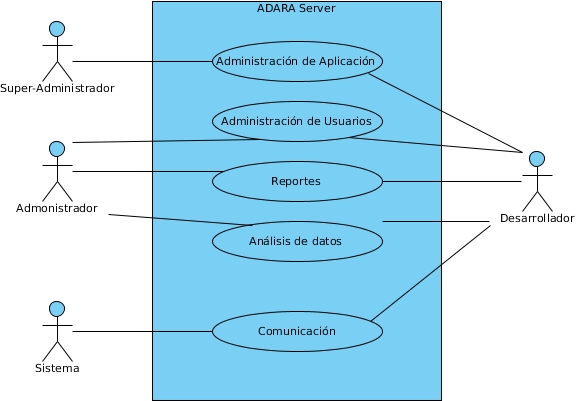
\includegraphics[width=0.75\textwidth]{./img/CUServidor.jpg}
\caption{ADARA Servidor}
\end{center}
\end{figure}






%\section{Diagramas de alto nivel}
%\subsection{Introducción}




%\section{Diagramas detallados}

%\section{Módulos}




\section{Cliente}

El cliente es una capa sobre Android que permite la realización de aplicaciones
de realidad aumentada, consiste de 5 componentes, los componentes son
librerías independientes que comunican entre ellos a través de interfaces y  se
configuran por medio de anotaciones, estos son los únicos componentes en ADARA
que no se comunican por medio de servicios web REST, esto debido a que de
serializar y deserializar objetos conlleva costo adicional que una
aplicación en tiempo real no se puede permitir.

ADARA Cliente esta compuesto por los siguientes componentes:
\begin{itemize}
  \item Caching: Un sistema de caching basado en localización.
  \item Menú: Permite el despliegue de menús e información haciendo uso del
  procesador gráfico.
  \item Actividades de realidad aumentada: Provee de toda la configuración
  necesaria para crear un Activity de android que permita desplegar aplicaciones
  de realidad aumentada.
  \item Cargador de objetos 3D: Permite cargar objetos 3D con extensión obj así
  como texturas, también permite registrar los objetos junto con los marcadores
  y los menús en una instancia de ARToolkit, lo cual permite desplegar todos los
  elementos en pantalla por medio del procesador gráfico.
  \item Comunicación: Permite sincronizar, enviar y recibir datos con ADARA
  servidor.
\end{itemize}

La arquitectura de ADARA cliente se muestra en la figura 7.3.

\begin{figure}[ht]
\begin{center}
 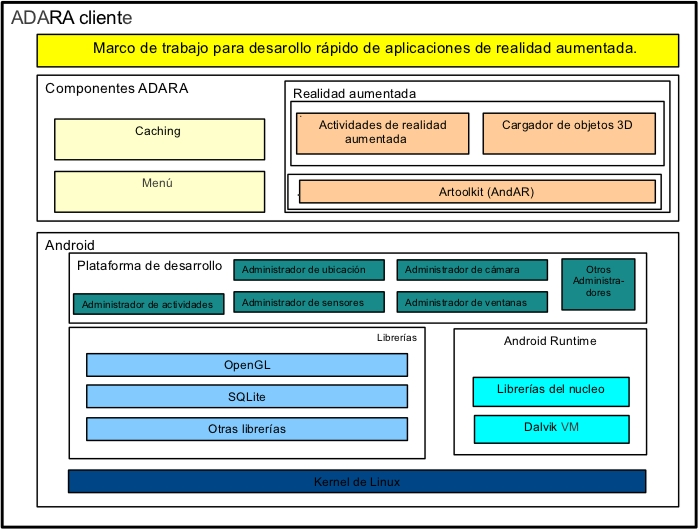
\includegraphics[width=0.95\textwidth]{./img/ADARACliente.jpg}
\caption{ADARA Cliente}
\end{center}
\end{figure}

Las configuraciones y los módulos se definen por medio de
anotaciones y el sistema las inyecta automáticamente en tiempo de compilación
por medio de AspectJ.


Existen dos métodos en donde se configuran los componentes adicionales:

El método configure de la clase AdaraActivity en donde se configuran los
componentes relacionados con ARtoolkit y componentes que no requieran hacer uso
del procesador gráfico.

El método draw de AdaraRenderer, en donde se deben de configurar los métodos que
requieran dibujar imágenes 2D o 3D con ayuda del procesador gráfico.


\subsection{Activity}
Un activity es un componente de android que proporciona una ventana sobre la
cual se despliega la interfaz de usuario, sobre la cual el usuario puede
realizar diferentes acciones de forma dinámica.
% en el apéndice C.2 se describen
%los principales métodos y el ciclo de vida del Activity.

Para el presente trabajo se hizo una implementación de Activity con todas las
funcionalidades y configuraciones necesarias para desplegar gráficas aumentadas
a la cual llamamos AdaraActivity.

Las funcionalidades de realidad aumentada se basan en AndAR, el cual es una
implementación para android de ARToolkit publicada bajo la licencia GPL, ADARA
no utiliza AndAR como si fuese una librería, en vez de eso extiende
algunas funcionalidades a nivel de código y hace algunas pequeñas
optimizaciones. 

\subsubsection{Propósitos}
Crear un Activity que permita desplegar los gráficos de aplicaciones de realidad
aumentada sin necesidad de configuraciones adicionales.

Tener un componente central, sobre el cual agregar diversos módulos.

\subsubsection{Implementación}

ADARA proporciona un Activity con todas las configuraciones necesarias para el
despliegue de aplicaciones de realidad aumentada llamado AdaraActivity.
AdaraActivity extiende la clase AndARActivity, que a la vez extiende la clase de
android Activity.

Para crear un Activity de realidad aumentada personalizado, sólo es necesario
extender la clase AdaraActivity.

AdaraActivity es el componente central de Adara Cliente, permite definir los
componentes adicionales, así como sus atributos.


Cuando se crea un Activity lo primero que se hace es configurar una instancia de
ARtoolkit para poder utilizar funcionalidades de realidad aumentada, después se
configuran los demás elementos como un objeto observable y los componentes
adicionales, también tiene la opción de precargar objetos 3D, que vayan as ser
usados posteriormente en la aplicación, a continuación entra en un ciclo en el
que  obtiene un frame, busca marcadores, en caso de encontrarlos ejecuta el
método draw de AdaraRenderer que usualmente se encarga de modificar las
matrices, al final despliega los gráficos en tiempo real, el número de frames
por segundo puede ser configurado mediante la anotación @FPS.

La figura 7.4 describe este proceso.



\begin{figure}[ht]
\begin{center}
 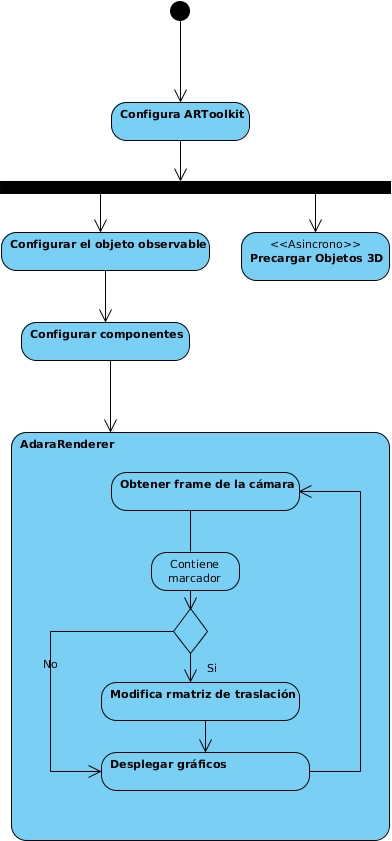
\includegraphics[width=0.4\textwidth]{./img/activityActivity.jpg}
\caption{Diagrama de actividades de AdaraActivity}
\end{center}
\end{figure}



AdaraActivity proporciona las siguientes funcionalidades:
\begin{itemize}
  \item Despliegue de gráficos en tiempo real por medio de OpenGL: Al igual que
  AndAR, ADARA delega las funcionalidades de despliegue de gráficos a una clase
  auxiliar llamada AdaraRenderer, esta se encarga de realizar todos los
  procedimientos que requieran hacer uso del procesador gráfico; AdaraRenderer
  es una implementación de OpenGLRenderer.
  \item Configuración de otros componentes: El método configure() provee de una
  forma sencilla para indicarle al sistema que componentes debe de usar.  
  \item Interacción en tiempo real con los usuarios: Siguiendo el patrón
  Observador, se genera una clase que notifica a el sistema cuando un usuario
  toca la pantalla táctil, indicando en tiempo real, las coordenadas a todos las
  clases que estén suscritas.  
  \item Implementación y configuración de ARToolkit: ADARA  genera y configura
  una instancia de ARtoolkit de forma automática  
  \item Precargado de objetos 3D: La creación de objetos 3D es un proceso que
  demanda una gran cantidad de recursos, esto obliga a poner la aplicación en
  espera en lo que se realiza este proceso, esto puede ser molesto para el
  usuario; con el fin de eliminar esta desventaja ADARA permite precargar
  objetos 3D de forma asíncrona, seleccionando los objetos que tengas mas
  probabilidades de ser usados basándose en las coordenadas pre-definidas de
  los objetos y en la ubicación del usuario obtenida por medio del GPS.
\end{itemize}

Como comentábamos AdaraRenderer se encarga de ejecutar todos los procesos que
requieran de aceleración por medio de gráficas. Consta de tres métodos, los
cuales ya contienen una implementación por defecto, sin embargo estas pueden ser
sobre-escritas para agregar características personalizadas.
Los métodos son los siguientes:
\begin{itemize}
  \item draw(): Es llamado cada que se despliega un nuevo frame.
  \item setuEnv(): Es llamado antes de dibujar los objetos, normalmente usado
  para definir la iluminación.
  \item initGL: Se llama cuando la superficie de OpenGL es inicializada.
\end{itemize}

El diagrama de clases de AdaraActivity se muestra en la figura 7.5.


\begin{figure}[ht]
\begin{center}
 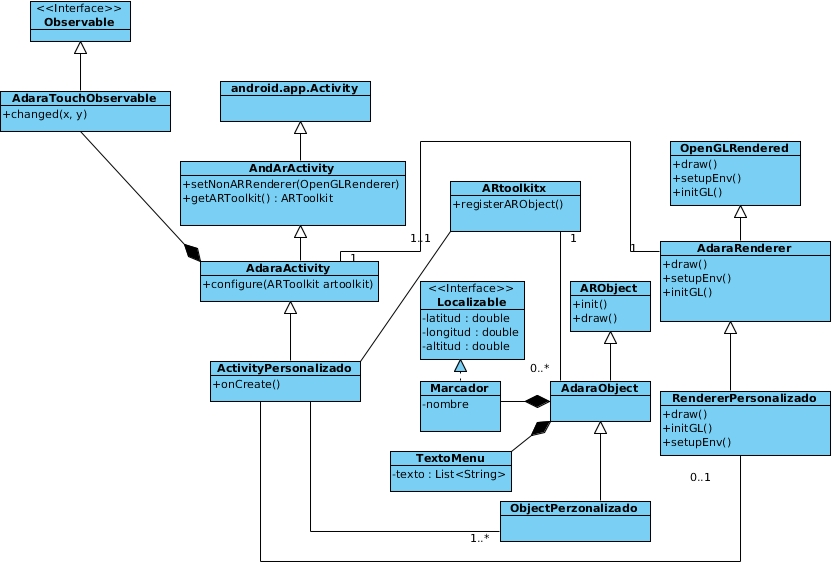
\includegraphics[width=0.85\textwidth]{./img/clasesActivity.jpg}
\caption{ADARA Cliente}
\end{center}
\end{figure}







%Esto va en menús
%@PreloadBaseTextTexture(true)
%FALTA:
%ARObject
%ARToolkitx
\subsubsection{Ventajas}

Activity listo para la creación y despliegue de gráficas por medio de OpenGL.

ARtoolkit configurado por defecto.

Permite al desarrollador enfocarse en las creación, despliegue  y en la
interacción de la aplicación con los usuarios, en vez de ejecutar acciones
mecánicas.

Vincula tecnologías probadas y robustas que cuentan con una gran comunidad de
desarrolladores.

Inyección de módulos en tiempo de compilación por medio de AspectJ. 

El desarrollador no requiere de conocimientos en ARToolkit.




\subsection{Menús}
ADARA menú es una librería de android que provee un componente que permite el
despliegue de información en menús, estos son dibujados por medio del procesador
gráfico.
\subsubsection{Propósitos}
Proveer un componente que permite desplegar información sobre objetos físicos en
la pantalla de un dispositivo móvil, la información debe ser generada en tiempo
real y desplegada por medio del procesador gráfico.

El componente debe ser independiente, fácilmente configurable y seguir el
paradigma de convención sobre configuración.

\subsubsection{Implementación}

Adara Menú requiere de una instancia de OpenGL para funcionar, esto es debido el
despliegue de las imágenes se hace por medio del procesador gráfico, un menú
esta compuesto internamente, por una textura de fondo más una textura por cada
renglón de cada opción.

Para el dibujado de los menús se sigue el siguiente algoritmo; a partir del punto
2 todas las acciones se ejecutan de manera repetitiva cada vez que se dibuja un
frame nuevo.

\begin{enumerate}
  \item Se cargan las texturas de fondo, estas contienen el diseño del menú,
  pueden ser vistos como menús sin información.
  \item  Se obtiene la orientación del dispositivo.
  \item Se obtiene un arreglo con los textos que van a ser desplegados, cada
  elemento del arreglo se relaciona con el texto de una opción del menú.
  \item Con la orientación y el número de elementos del arreglo se selecciona la
  textura de fondo que mejor se adapte.
  \item Se calcula el tamaño y la posición del menú.
  \item Se despliega la textura de fondo.
  \item Se calcula el tamaño máximo de cada renglón, se dividen los textos en
  subtextos que se puedan desplegar en un renglón
  \item Se verifica en un objeto caché que las texturas requeridas no hayan sido
  usadas previamente.%=====%
  \item Se crea un mapa de bits con un valor alfa de 0 (transparente) por cada
  renglón que no haya sido creado previamente y se le agregan los textos.
  \item Se cargan las textura y se guardan los identificadores en un caché.
  \item Se calcula la posición de las texturas con texto.
  \item Se despliegan las texturas.
\end{enumerate}

La figura 7.6 nos muestra un diagrama de actividades simplificado de Adara
Menú.



Si se desea modificar el componente menú por uno personal solo es necesario
implementar la interfaz AdaraMenu, aunque por defecto contamos con una
implementación de dicha interfaz , en la figura 7.7 podemos observar el diagrama
de clases.





Adara Menú registra al objeto observable implementado por Adara Activity, con
el fin de obtener la ubicación de los \emph{clicks} en la pantalla táctil.
 
 Para activar o desactivar el módulo menú solo es necesario definir la anotación
 @DrawMenu(true) en el método draw de la clase AdaraRenderer.


La configuración de las características del menú se hace por medio de la
anotación  @MenuConfiguration sobre el método drawMenu de la clase MenuFacade,
como se muestra en el siguiente ejemplo.


\newpage
\begin{verbatim}
 @MenuConfiguration
    (
            textSize = 20,  
            ARGBColor = {0xff,0x00,0x00,0x00},
            antiAlias = true,
            fontFamily = "normal",
            fontStyle = Typeface.NORMAL,
            widthPercentage = .9f,
            heightPercentage = .25f         
    )
    public void drawMenu(GL10 gl) throws JaguARException{
        ...
    }
    \end{verbatim}


\begin{figure}[ht]
\begin{center}
 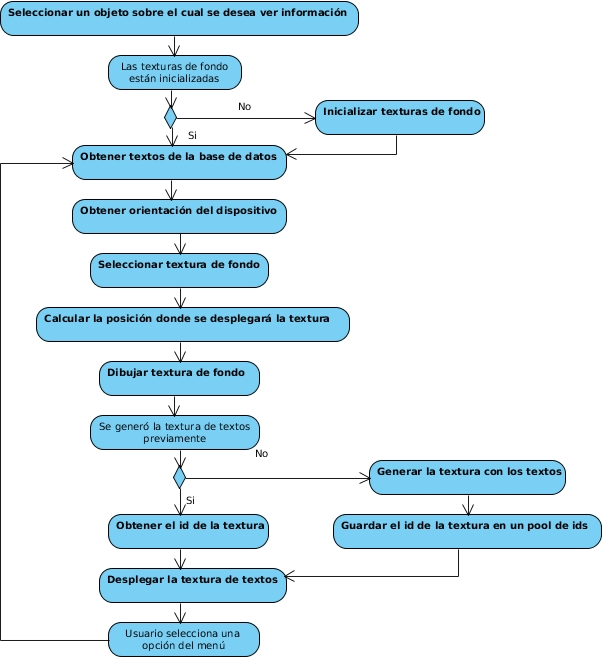
\includegraphics[width=0.7\textwidth]{./img/menuActivity.jpg}
\caption{Diagrama de actividades de Adara menú}
\end{center}
\end{figure}

\begin{figure}[ht]
\begin{center}
 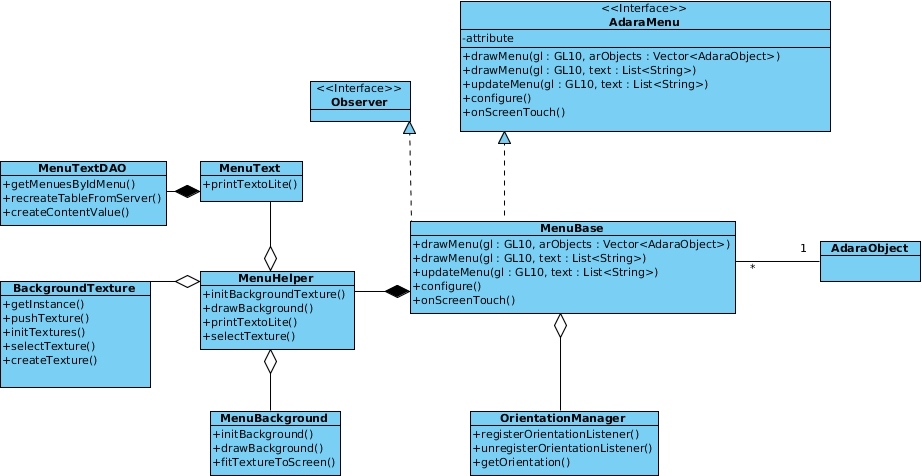
\includegraphics[width=0.9\textwidth]{./img/menuClases.jpg}
\caption{Diagrama de clases de Adara menú}
\end{center}
\end{figure}


\subsubsection{Ventajas}

Maneja la rotación de las pantallas de android.

Contiene un pool de texturas que permite reutilizarlas.

Genera varias texturas pequeñas, de una linea, que aumentan la probabilidad de
Reutilización de estas y evita así generar nuevas texturas.

Pre-carga las texturas de fondo, lo que permite reducir el tiempo de despliegue. 

Soporta los mismos caracteres que el teléfono.



\subsection{Caching}
ADARA también provee un módulo de caching, el cual es utilizado por Adara
menú y Adara 3dLoader, este módulo fue explicado en el capítulo 6.


\subsection{Carga de objetos 3D}
Adara 3DLoader esta basado en ModelLoader de Thobias Domham \cite{aroasf}, el
cual permite cargar objetos .obj y texturas,  ModelLoader no es una librería,
sino una aplicación que no podía utilizarse de forma independiente y sólo
cargaba objetos 3D predefinidos, se modifico este comportamiento a nivel de
código para que permitiera integrarse con otros módulos y cargar objetos de
forma dinámica.

\subsubsection{Propósitos}
Tener un componente que permita la creación de objetos 3D, configurarlo para que
funcione con ARToolkit y desplegarlos por medio del procesador gráfico.

Tener un componente que ayude en la configuración de marcadores, menús y objetos
en una instancia de ARtoolkit.

\subsubsection{Implementación}

Existen tres funcionalidades de Adara 3DObject, las cuales se describen a
continuación:

\begin{itemize}
  \item Cargar objetos 3D:  Permite cargar tanto objetos internos, como
  externos. Los objetos internos deben de estar en el folder asset, es imposible
  cargar estos objetos de forma dinámica debido a que los elementos en este
  folder forman parte del .apk (formato de empaquetado que realiza la misma
  funcionalidad del jar de java) de android, por lo tanto no se pueden agregar
  objetos a este folder en tiempo de ejecución. Los objetos externos pueden
  estar en cualquier lugar disco dentro de java, incluso en servidores externos,
  sin embargo sólo se recomienda su utilización en casos excepcionales debido a
  que el tiempo de procesamiento se eleva.
  
  \item Registrar objetos 3D en ARtoolkit: Permite registrar objetos en una
  instancia de ARtoolkit y cargarse de forma asíncrona.
  
  \item Configurar marcadores, menús en Artoolkit.
\end{itemize}



La figura 7.8 muestra el diagrama de clases de Adara 3DLoader.
\begin{figure}[ht]
\begin{center}
 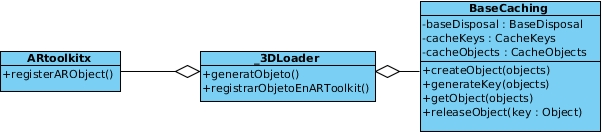
\includegraphics[width=0.7\textwidth]{./img/clasesLoader.jpg}
\caption{Diagrama de clases de Adara 3DLoader}
\end{center}
\end{figure}


Adara 3dLoader permite configurar objetos en una instancia de ARTookit, antes de
que estos sean cargados en el procesador gráfico, en caso de que se requiera
desplegar el objeto sin que haya sido completamente creado, se despliega en su
lugar un objeto por defecto, el cual se empieza a cargar de forma asíncrona al
momento de generar una instancia de \_3DLoader, la figura 7.9 muestra un
diagrama de actividades en donde se puede apreciar la forma en como se configuran los
objetos obtenidos por 3DLoader en ARToolkit. La figura 7.10 describe la forma en
como se generan los objetos en 3DLoader.

\begin{figure}[ht]
\begin{center}
 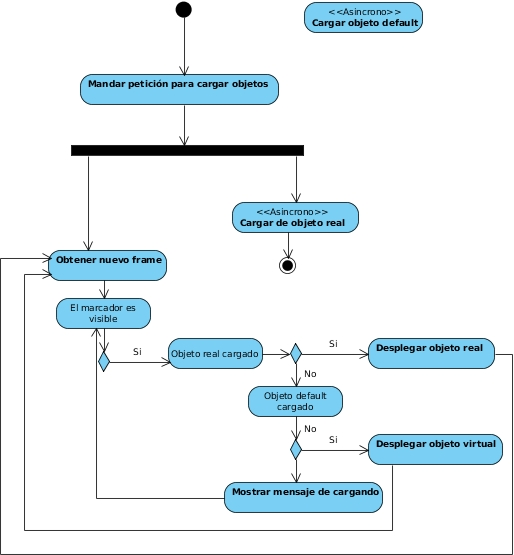
\includegraphics[width=0.6\textwidth]{./img/activityLoader1.jpg}
 \caption{Diagrama de actividades de configuración de objetos 3D en ARtoolkit}
\end{center}
\end{figure}

\begin{figure}[ht]
\begin{center}
 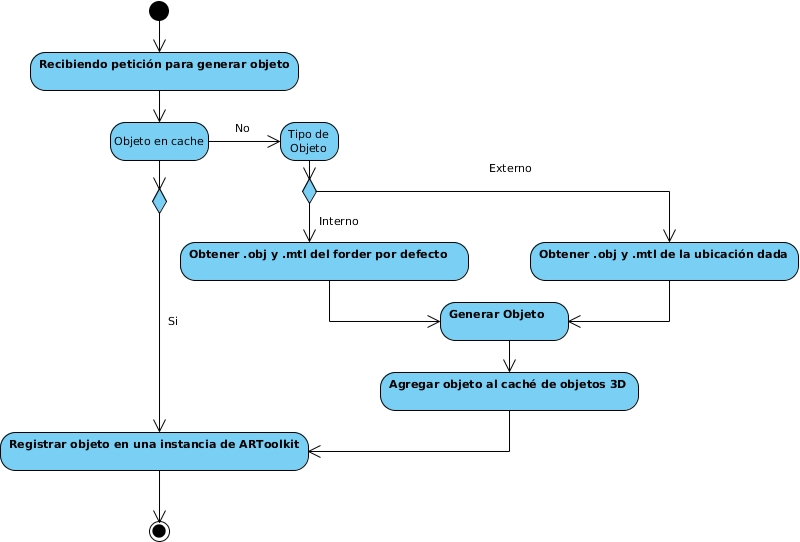
\includegraphics[width=0.7\textwidth]{./img/activityLoader2.jpg}
 \caption{Diagrama de actividades de la generación de objetos de 3DLoader}
\end{center}
\end{figure}



\subsubsection{Ventajas}
Permite la fácil creación, despliegue y eliminación de objetos 3D con extensión
obj.

Caching automático de objetos, eliminación basada en localización.

Permite configurar objetos 3D en una instancia de ARToolkit.


\section{Servidor}


ADARA servidor compuesto por los siguientes componentes:

\begin{itemize}
  \item Administración de usuarios: Permite relacionar usuarios, la información
  y los objetos 3D que van a ser desplegados.
  \item Administración de aplicación: Permite generar instancias independientes,
  administrar los permisos de usuarios y organizaciones, agregar información y
  objetos 3D.
  \item Reportes: Permite generar reportes sobre la actividad de los usuarios.
  \item Análisis de datos: Permite generar los reportes sobre las actividades
  más realizadas, los módulos más usados, tiempo de respuesta de diferentes
  módulos y demás información que permita detectar cuellos de botellas y formas
  de optimizar la aplicación.  
\item Comunicación: Permite sincronizar, enviar y recibir datos con ADARA
cliente.
\end{itemize}

La arquitectura de ADARA servidor se muestra en la figura 7.11.

\begin{figure}[ht]
\begin{center}
 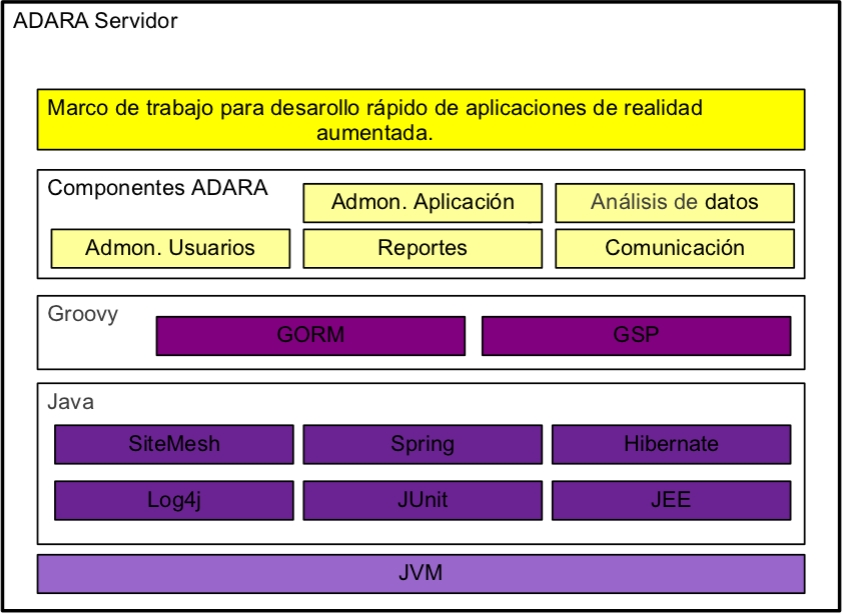
\includegraphics[width=0.95\textwidth]{./img/ADARAServidor.jpg}
\caption{ADARA Servidor}
\end{center}
\end{figure}

\subsection{Plugin grails}
Un plugin de grails puede ser definido como un componente que agrega
características especiales a una aplicación más grande, permiten integrar
funcionalidades de terceros a una aplicación, de  una forma parecida a como lo
hace una librería, pero con la ventaja de que no solo permite agregar clases,
también es posible agregar jars, GSP, modelos, controladores, tagLibs,
servicios, etc, por medio de plugins es posible  unir dos aplicaciones y
convertirlas en una sola. Esto permite enfocarse en los requerimientos
funcionales de la aplicación y agregar funcionalidades adicionales
desarrolladas por terceros para realizar tareas especificas o mecánicas.

\subsubsection{Propósitos}
Crear un plugin que permita tener tener una instancia de Adara servidor
completamente funcional lista en minutos.

\subsubsection{Implementación}
Se creó un plugin de grails que permite mediante la instrucción grails
instal-plugin adaraServer descargar, instalar y configurar todos los componentes
necesarios para tener una instancia de ADARA server completamente funcional.
Los componentes que se instalarán son los que se describen en las siguientes
subsecciones.

Se puede tener una instalación mínima funcional en 10 simples pasos.

\begin{enumerate}
  \item Crear una aplicación de grails que sirva de anfitrión para ADARA
  administración de aplicación.
  \item Instalar el plugin de adara administración de aplicación.
  \item Desplegar  ADARA administración de aplicación.
  \item Introducir los datos deseados (la interfaces se crearon al momento de
  instalar el plugin).
  \item Crear una aplicación de grails que sirva de anfitrión para ADARA
  administración de usuario.s
  \item Instalar el plugin de adara administración de usuarios.
  \item Crear una clase de tipo controlador y agregarle una valiable estatica
  llamada urlServer que indique la url de ADARA administración aplicación.
  \item Desplegar la aplicación.
  \item Desplegar  ADARA administración de usuarios.
  \item Introducir los datos deseados.
\end{enumerate}

\subsubsection{Ventajas}
Tener toda la implementación y configuración de ADARA server lista en poco
tiempo.

La descarga es a nivel de código, por lo cual se pueden modificar los
componentes.



\subsection{Análisis de datos}
Permite recolectar información sobre el tiempo que tardan en ejecutarse los
métodos en AdaraCliente.

\subsubsection{Propósitos}
Tener información sobre que métodos y/o clases son más usadas, y el
tiempo que tardan en ejecutarse, con el fin de usarlos para la optimización de
la aplicación.

\subsubsection{Implementación}
%Permite agregar en tiempos de compilación 

Obtiene la hora de inicio y de finalización de un un método, calcula el tiempo
que se tardó en ejecutar y lo guarda junto con el nombre del método y de la
clase en una base de datos local, cuando encuentra una conexión
disponible envía esta información al servidor.

Se genera una vista con los reportes, los  cuales pueden ser exportados a
diversos formatos, entre ellos pdf, xml y rtf, esta funcionalidad se logra por
medio un plug-in de grails llamado export plugin.

Para que un método sea reportado simplemente se necesita agregar la anotación
@Trace y la funcionalidad anteriormente descrita se inyectará en tiempo de
ejecución mediante AspectJ.

La figura 7.12 muestra un diagrama de actividades que describe la forma en como
funciona este módulo.  

\begin{figure}[ht]
\begin{center}
 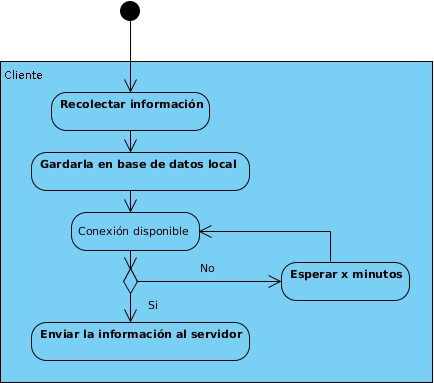
\includegraphics[width=0.45\textwidth]{./img/activAnalysis.jpg}
\caption{diagrama de actividades de análisis de datos}
\end{center}
\end{figure}



\subsubsection{Ventajas}

Este módulo permite identificar los cuellos de botella, que componentes no están
funcionando correctamente y en donde es más conveniente optimizar.
 

 
 %AL FINAL SI DA TIEMPO XD   
%\subsection{Reportes}
%\subsubsection{Introducción}
%Permite generar información sobre la forma en que los usuarios usan la
%aplicación.

%\subsubsection{Propósitos}
%\subsubsection{Implementación}
%\subsubsection{Aportes}
%\subsubsection{Conclusión}

\subsection{Administración de aplicación}
Este es un módulo que permite administrar diferentes instancias de la aplicación,
y proveer a la aplicación los datos necesarios para su funcionamiento,
prácticamente se trata de operaciones de creación, obtención, actualización y
eliminación (CRUD) de algunas de las tablas que se muestran en el diagrama
entidad relación. 
Para usar este módulo se tienen que tener permisos de súper usuario. 

\subsubsection{Propósitos}
Proveer a ADARA Cliente de los datos necesarios para su funcionamiento y
configuración.

Entre sus funciones se encuentra: 

\begin{itemize}
  \item CRUD instancias independientes
  de aplicaciones de realidad aumentada
  \item CRUD compañías
  \item CRUD usuarios
  \item CRUD secciones (relacionadas con una compañía)
  \item CRUD objetos3D.
  \item CRUD menús.
  \item CRUD marcadores.
  \item CRUD dispositivos
  \item CRUD sistemas operativos
\end{itemize}

\subsubsection{Implementación}

Grails, por medio de GORM permite la creación automática de operaciones CRUD
siguiendo una serie de reglas, solo es necesario indicar las clases de dominio,
también se pueden indicar las relaciones por medio de closures. Se hará uso de
esta característica para generar las funcionalidades de este módulo.
% el ápendice
%E.1 explica la forma en como funciona y las reglas que se tienen que
%seguir. 


\subsection{Administración de usuario}
En este módulo se definen las asociaciones entre los diferentes elementos de
realidad aumentada, principalmente los siguientes:
\begin{itemize}
  \item \_3DObjets: Que objeto va a ser desplegado.
  \item Markers: Cual es el marcador que se tiene que encontrar para que el
  objeto sea desplegado.
  \item Menu: Cuales son los textos que se van a desplegar.
  \item Localization: Cual es la localización en donde se encuentra el marcador.
  \item Usuario: Que usuarios son afectados por una configuración dada.
\end{itemize}


\subsubsection{Propósitos}
Definir las relaciones entre usuarios, objetos 3D, marcadores y textos de
menú.

\subsubsection{Implementación}

Al igual que el módulo de administración de la aplicación, este módulo se genera
principalmente por medio de grails y GORM.

\subsection{Comunicación}
El módulo de comunicacíon permite sincronizar los datos del cliente con los del
servidor y viceversa.
\subsubsection{Propósitos}

Permitir mandar datos almacenados en el cliente al servidor.

Permitir sincronizar un subconjunto de los datos almacenados en el servidor con
las tablas de configuración de los datos en el cliente.

\subsubsection{Implementación}
La sincronización se hará entre la base de datos nativa de Android (SQLite) y
cualquier base de datos del servidor que sea soportada por GORM (Hibernate).

 
Este módulo se basa principalmente en tres tecnologías:

\begin{itemize}
  \item JSON REST api plugin: Permite definir las interfaces REST en el
  Servidor.
  \item Spring android REST Template: Permite definir las interfaces REST en el
  cliente.
  \item Android C2DM: Facilita la implementación de peticiones tipo \emph{push}.
\end{itemize}
\setstretch{1.15}
%Si da tiempo podemos poner un anexo con la forma de utilizar estas tecnologías.
Estas tecnologías facilitan el desarrollo del presente módulo, sin embargo para
que el módulo cumpla con las restricciones de la arquitectura REST, las
implementaciones son definidas por los desarrolladores, por lo tanto el único
requisito necesario es exponer las interfaces de forma correcta. En este módulo
se definirán dos interfaces, la primera sirve para el envío de información entre
cliente y servidor, el formato se especifica en el código 7.1.




 
\begin{verbatim}
{
    "user":"nombreUsuario",
    "password":"passwordUsuario",
    "database":"nombreBaseDeDatos",
    "data":
        [
            {
                "nombreCampo":1,
                "nombreCampo":"q",
                "nombreCampo":true
            },
            {
                "nombreCampo":2,
                "nombreCampo":"x",
                "nombreCampo":false
            }
        ]
}

Código 7.1: Formato de JSON para envío de información entre
    el cliente y el servidor. 
\end{verbatim}




Tambien se debe implementar una segunta interfaz que permite obtener los
campos y los tipos de datos en caso de que sea necesario recrear las tablas o
las bases de datos, el formato se define en el código 7.2. 
Por seguridad todos las peticiones deben de autenticarse y la contraseña debe de
mandarse de forma encriptada.

Los datos que se envían del cliente al servidor pueden contener un campo con la
fecha en la que dichos datos fueron recolectados, los posibles errores asociados
al uso de diferentes relojes físicos son minimizados haciendo uso del
algoritmo de Christian para sincronización de relojes.
Por defecto si no se especifica el nombre de la base de datos y de las tablas se
utilizan los nombre originales.
\newpage

\begin{verbatim}
{
    "user":"nombreUsuario",
    "password":"passwordUsuario",
    "database":"nombreBaseDeDatos",
    "table":"nombreTabla",
    "fields": 
        [ 
            { name: 'nombreDelCampo', type: 'tipoDelCampo' }, 
            { name: 'nombreDelCampo', type: 'tipoDelCampo' }, 
            { name: 'nombreDelCampo', type: 'tipoDelCampo' } 
        ]
}
Código 7.2: Formato de JSON para obtener el nombre de los campos y tablas.
\end{verbatim}



El sistema provee de una funcionalidad para la creación automatica de interfaces
REST que cumplan con los requerimeintos definidos, solo es necesario seguir los
siguentes pasos:

\begin{itemize}
  \item Servidor.
    \begin{itemize}
        \item Crear un controlador.
        \item Definir una variable estática llamada json que contenga el objeto
        que se desea enviar.
    \end{itemize}
    \item Cliente.
    \begin{itemize}
        \item Registar las peticiones \emph{push}.
        \item Crear una clase en el paquete *.adara.rest
        \item Definir una variable estática llamada AdaraSincronization y
        pasarle como valor la URL a la que se van a enviar los datos.
        \item Agregar una anotación llamada AdaraSincronization y
        pasarle como valor la URL a la que se van a enviar los datos.
    \end{itemize}   
\end{itemize}


Tanto en el cliente como en el servidor se inyectarán las funcionalidades
necesarias en tiempo de compilación, en el servidor haciendo uso de la
metaprogramación de grails y el el cliente gracias a AspectJ.



\subsubsection{Ventajas}
Permite enviar datos de forma remota del cliente al servidor.

Permite sincronizar y actualizar la base de datos del cliente con un subconjunto
de la base de datos del servidor.

Permite la comunicación entre componentes del cliente y del servidor.

Creación automatica de interfaces REST.

\singlespacing


%\chapter{Pruebas}
%\section{Técnicas}
%\section{Pruebas de campo}
%\newpage


%CaSO
\chapter{Caso de estudio y resultados}
%\section{Características del prototipo}
%\subsection{S.O.}
%\subsection{Sensores}
%\subsection{Cámara}
%\subsection{Procesamiento}

%\section{Características del prototipo}

\section{Introducción}

Durante el desarrollo de ADARA se identificarón las principales características
que mermaron la productividad en su desarrollo, y se propusieron como métricas
para probar el grado de completez de la hipótesis. Estas fueron:

\begin{itemize}
  \item Curva de aprendizaje: Cuanto tiempo requiere aprender a utilizar las
  tecnologías requeridas para la creación de una aplicación de realidad
  aumentada.
  \item Tiempo de desarrollo: Tiempo invertido en la creación de una aplicación
  de realidad aumentada.
  \item Tecnologías: Cantidad de tecnologías necesarias para poder desarrollar
  una aplicación de realidad aumentada.
  \item Facilidad para agregar nuevos componentes.
  \item Enfoque en objetivos de negocio: Relación entre el tiempo usado en el
  desarrollo de procesos de negocio y la configuración de la aplicación.
 % \item Instalación de ambiente y liberación: Tiempo requerido para crear el
  %esqueleto de la aplicación.   
\end{itemize}

\section{Escenario}
El presente caso de estudio compara el desarrollo tradicional de una aplicación
de realidad aumentada y el desarrollo por medio de ADARA. Ambos desarrollos
fueron realizados por una sola persona, con el apoyo de un asesor.

Como ejemplo de aplicación por medios tradicionales se uso el desarrollo de
ADARA, el cual es en si mismo una aplicación de realidad aumentada.

Para analizar el funcionamiento de ADARA, se creó una implementación de esta,
con las siguientes características.

Aplicación cliente-servidor que permita ver las característica de un
dispositivo (computadora, impresora, etc). La
aplicación móvil al detectar un dispositivo con un marcador asociado debe ser
capaz de desplegar información relativa a este, así como un menú interactivo que
permita al usuario ver los detalles específicos de cierta característica (Ver
fig. 8.1). Los datos que alimentan a el cliente se deben de suministrar por
medio de una aplicación web (Ver fig 8.2).


\begin{figure}
\begin{center}
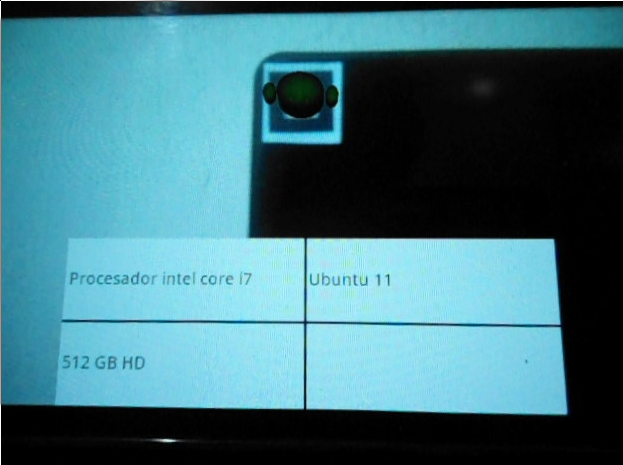
\includegraphics[width=0.4\textwidth]{./img/cliente1.jpg}
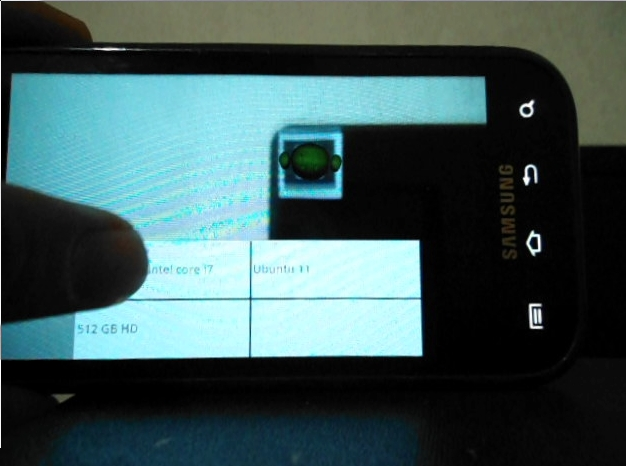
\includegraphics[width=0.4\textwidth]{./img/cliente3.jpg}
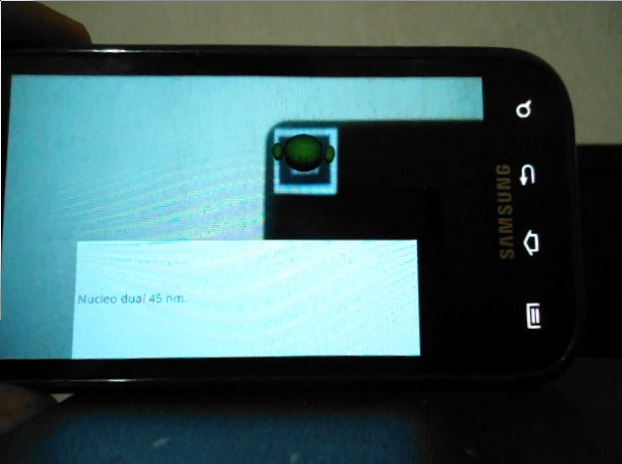
\includegraphics[width=0.4\textwidth]{./img/cliente4.jpg}
\caption{Implementación de ADARA Cliente}
\end{center}
\end{figure}



\begin{figure}
\begin{center}
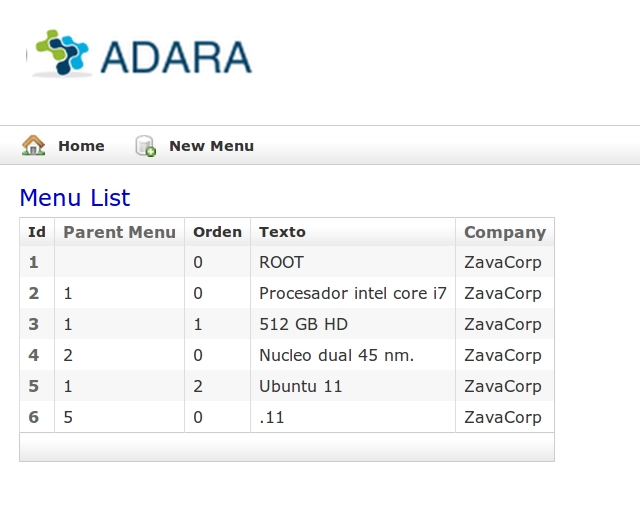
\includegraphics[width=0.4\textwidth]{./img/servidorAdmin1.jpg}
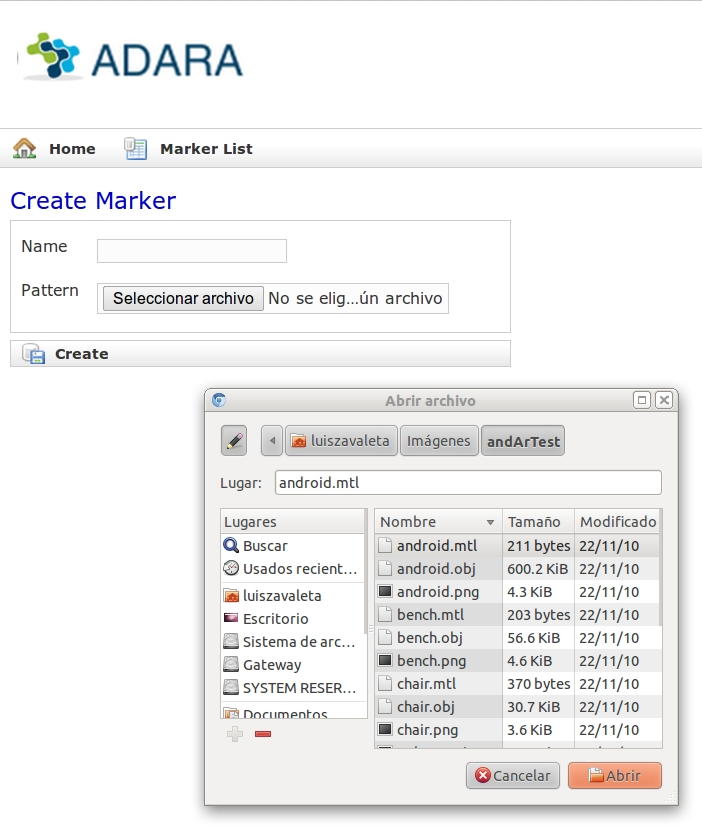
\includegraphics[width=0.4\textwidth]{./img/servidorAdmin2.jpg}
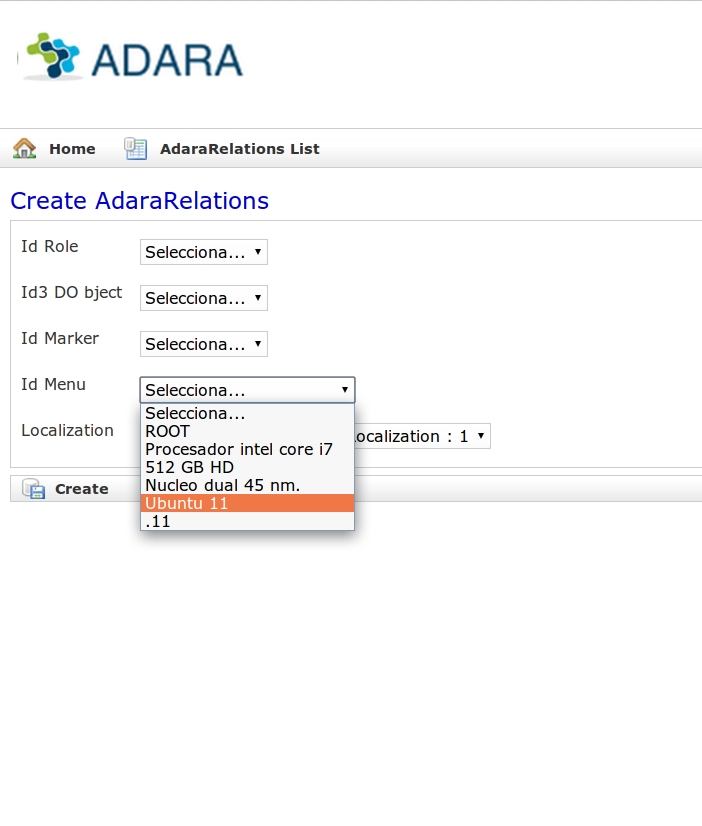
\includegraphics[width=0.4\textwidth]{./img/servidorUser.jpg}
\caption{Implementación de ADARA Servidor}
\end{center}
\end{figure}










\section{Curva de aprendizaje}
\subsection{Desarrollo tradicional}
La curva de aprendizaje fue muy elevada, debido principalmente a las siguientes
razones:
\begin{itemize}
  \item Falta de conocimiento de OpenGL por parte del desarrollador.
  \item Necesidad de hacer uso de diversas tecnologías para poder lograr los
  objetivos.
  \item Aunque se baso en AndAR, se requería entender como funcionaba el código
  de las principales clases para poder extender su funcionalidad.

\end{itemize}

\subsection{Soluciones proveídas por ADARA}
\subsubsection{Falta de conocimiento de OpenGL por parte del desarrollador}
ADARA Provee un módulo para crear objetos 3D, registrarlos en una
instancia de ARtoolkit, desplegarlos en pantalla y otro que permite desplegar
información asociada a estos, todo por medio del procesador gráfico, por lo que
no es obligatorio conocer OpenGL, sin embargo, si se desea
modificar o mejorar esta funcionalidad, solamente es necesario modificar o
substituir los módulos correspondientes ya sea agregando el código
necesario para cubrir los requerimientos en el método draw de AdaraRenderer, o
inyectandolo por medio de AspectJ.

\subsubsection{Necesidad de hace uso de diversas tecnologías para poder lograr los
  objetivos}
  ADARA permite que el usuario solamente se enfoque en las tecnologías de las
  cuales es experto, proveyendo funcionalidades por defecto para las restantes.

\subsubsection{Necesidad de entender como funcionaba el código
  de las principales clases para poder extender alguna funcionalidad}
  ADARA provee en la parte del cliente interfaces bien definidas que
  permiten al desarrollador extender fácilmente las funcionalidades, además la
  mayoría de las configuraciones son por medio de anotaciones y las
  funcionalidades se inyectan al código en tiempo de compilación, por lo que
  solo es necesario seguir las reglas proveídas para extender dichas funcionalidades. En la parte del
  servidor toda la comunicación es por medio de servicios web REST, lo que permite enfocarse simplemente en proveer las interfaces adecuadas, sin que
  sea necesario saber la forma en como fueron implementadas, el lenguaje, la
  arquitectura interna, etc.
\subsection{Desarrollo por medio de ADARA}

La curva de aprendizaje fue baja debido a las siguientes razones:
\begin{itemize}
  \item Reduce sustancialmente el número de configuraciones necesarias.
  \item Las pocas configuraciones requeridas se hacen por medio de anotaciones.
  \item Se basa en tecnologías usadas por con una gran cantidad de
  desarrolladores y con diversos libros y tutoriales acerca de ellas.
  \item No es necesario saber todas las tecnologías para poder crear una
  aplicación de realidad aumentada.
\end{itemize}



\section{Tiempo de desarrollo}
\subsection{Desarrollo tradicional}
Se invirtieron aproximadamente 350 horas en el desarrollo y 250 en dominar las
tecnologías necesarias.
\subsection{Desarrollo por medio de ADARA}
Se invirtieron 90 horas en el desarrollo, no se requirió de aprender tecnologías
nuevas, debido a que esta basado en estándares de facto.

\section{Tecnologías}
\subsection{Desarrollo tradicional}
Se requirió tener conocimientos en las siguientes tecnologías:
\begin{itemize}
  \item Cliente
  \begin{itemize}
    \item Java
    \item OpenGL
    \item ARToolkit
    \item Android
    \item SQLite
    \item POO
    \item POA
    \item POC
  \end{itemize}
 \item Servidor
  \begin{itemize}
    \item Groovy
    \item Grails
    \item GSP
    \item REST
    \item Export plugin
    \item Spring
    \item SiteMesh
    \item Hibernate
    \item POO
    \item POA
  \end{itemize}
\end{itemize}

\subsection{Desarrollo por medio de ADARA}
Aunque usa las mismas tecnologías solo se requiere saber como usar las que se
necesiten para un módulo especifico, incluso en la parte del servidor es posible
utilizar otras tecnologías o lenguajes ya que el funcionamiento se basa
únicamente en la correcta implementación de las interfaces.



\section{Facilidad para agregar nuevos componentes}
\subsection{Desarrollo tradicional}
Para agregar un componente primero se requiere saber como esta desarrollada la
aplicación, las tecnologías que usa, entender los diagramas disponibles
(generalmente no existen) y analizar y comprender la aplicación a nivel de
código.
\subsection{Desarrollo por medio de ADARA}
En el cliente solo es necesario configurar los nuevos componentes por medio de
anotaciones e inyectar las funcionalidades por medio de AspectJ en los métodos
draw para módulos relacionados directamente con OpenGL o configure para lo
demás.

En el servidor el único requisito es la implementación correcta de interfaces de
REST.



\section{Enfoque en objetivos de negocio}
\subsection{Desarrollo tradicional}
Requiere implementar manualmente requisitos funcionales, no funcionales
y configuraciones.

\subsection{Desarrollo por medio de ADARA}
Hace posible enfocarse completamente en los objetivos del negocio y provee de
configuraciones y funcionalidades por defecto para algunos requisitos no
funcionales, se basa en tecnologías que permiten el desarrollo rápido de aplicaciones.

\section{Conclusión}
ADARA permite disminuir considerablemente los tiempos de desarrollo, debido a
esto evita la realización de actividades mecánicas y configuraciones
innecesarias, los desarrolladores pueden crear una aplicación muy rápidamente y
modificar u optimizar componentes específicos, utilizando sus conocimientos pre adquiridos
y dejando al sistema implementar las funcionalidades de las otras áreas. También
permite enfocar los esfuerzos a la implementación de la lógica del negocio.





\chapter{Conclusiones}

El presente trabajo tuvo como objetivo el desarrollo de un marco de trabajo
altamente productivo, el cual por medio del uso de estandares de facto,
metodologías de desarrollo ágil y tecnologías emergentes permite la creación de
aplicaciones de realidad aumentada. A dicho marco de trabajo se le nombro ADARA.

Para evaluar el marco de trabajo propuesto se definieron las siguientes
características:
\begin{itemize}
  \item Curva de aprendizaje.
  \item Tiempo de desarrollo.
  \item Cantidad de tecnologías requeridas.
  \item Facilidad para agregar nuevos componentes.
  \item Porcentaje de tiempo dedicado a la configuración.
\end{itemize}

Uno de los pasos más importantes fue la identificación de las tecnologías sobre
las cuales se realizo el marco de trabajo, con el fin de satisfacer los
objetivos planteados se tomaron en cuenta las siguientes características.

\begin{itemize}
  \item Tecnologías emergentes ampliamente usadas.
  \item De código abierto.
  \item Documentación disponible.
  \item Contar con una amplia comunidad de desarrolladores.
  \item Curva de aprendizaje baja
\end{itemize}

Además de seleccionar tecnologías que nos permitieran cubrir los requisitos
funcionales, también fue necesario identificar aquellas que nos permitieran
implementar elementos de configuración de forma dinámica, así como otras que
permitieran la fácil modularización de la aplicación.

Mediante una investigación bibliográfica se llego a la conclusión de que las
herramientas que mejor se adaptaban a las necesidades del presente trabajo son
las siguientes:

\begin{itemize}
  \item OpenGL ES 1: Estándar para desarrollo de aplicaciones gráficas 2D y 3D
  en sistemas integrados.
  \item AndAr: Implementación de ARToolkit para dispositivos con el sistema
  operativo Android.
  \item Servicios Web REST: Permite esconder los detalles de implementación de
  los componentes y enfocarse en las interfaces de comunicación.
  \item Android: Sistema operativo con un ambiente de desarrollo abierto 
  \item Grails: Marco de trabajo para desarrollo rápido de aplicaciones web,
  basado en tecnologías ampliamente usadas.
  \begin{itemize}
    \item Hibernate: Estándar de facto para el mapeo objeto-relacional (ORM) en
    Java.
    \item Spring: Framework muy popular para desarrollo de aplicaciones java con
    soporte para Inversión de control.
    \item Groovy: Lenguaje orientado a objetos, ágil y de tipado dinámico.
  \end{itemize}
  \item JSON: Formato de envío de mensajes compacto que permite la creación y
  lectura de archivos de forma eficiente, existen numerosas librerías en
  diversos lenguajes que permiten la serialización y deserialización de objetos.
  \item Grails plugin: Permiten integrar funcionalidades de terceros a una
  aplicación, de una forma parecida a como lo hace una librería, pero a
  diferencia de una librería permite integrar todos los elementos necesarios
  para tener una aplicación funcional
  \item AspectJ: Permite agregar funcionalidades de forma dinámica, en android
  sólo permite agregarlas en tiempo de compilación.
\end{itemize}


Una vez identificadas las tecnologías, se propuso una arquitectura la cual
pretende proporcionar una metodología y un marco de trabajo que facilite el
desarrollo de aplicaciones de realidad aumentada.

La arquitectura se basa principalmente en 3 pilares:

\begin{itemize}
  \item Convención sobre configuración: Con el fin de reducir considerablemente
  el tiempo usado en la configuración de la aplicación y centrarse en el
  desarrollo de los objetivos del negocio.
  \item Orientada a componentes: Facilita la modularización de los componentes,
  permite independizar los componentes de su implementación y centrarse en la
  definición de las interfaces.
  \item De código abierto: Permite el libre acecso al código fuente, lo que
  garantiza que los desarrolladores podrán mejorarlo o personalizarlo.
\end{itemize}


La arquitectura de ADARA cuenta con dos subsistemas, ADARA cliente y ADARA
servidor. 

ADARA Cliente se encarga del despliegue de gráficos en 2D y 3D, tanto
de los obtenidos por medio de la cámara como de los objetos e información
virtual adicional. Puede ser visto como una capa sobre Android.

ADARA Servidor permite la administración de los datos de la aplicación, de sus
usuarios, etc, así como la generación de reportes y el análisis de las
actividades de los usuarios, se comunica entre sus componentes y con ARADA Cliente por medio de Servicios Web REST.

Los objetivos específicos que se cumplen por medio de ADARA Cliente son los
siguientes:

\begin{itemize}
  \item Despliegue de información haciendo uso del procesador gráfico: Este
  objetivo se cumple gracias a dos componentes de ADARA Cliente.
    \begin{itemize}
    \item ADARA Activity: Clase que contiene todas las configuraciones
    necesarias para el despliegue de gráficos 2D y 3D por medio de OpenGL 1.0,
    también contiene por defecto una instancia de ARToolkit que permite la fácil
    implementación de aplicaciones de realidad aumentada. El principal aporte de
    este módulo es permitir a desarrolladores de OpenGL que deseen crear aplicaciones de
    realidad aumentada centrarse en la forma en como se despliegan los gráficos
    sin la necesidad de aprender otra tecnologías como Android o Java.
    \item ADARA Menú: Permite el despliegue de información en forma de menús,
    los menús se despliegan por medio del procesador gráfico. Sus principales
    características es la implementación de un pool de texturas de textos que
    permite reutilizar secciones de texto, el precargado de texturas de fondo y
    la generación de texturas de texto de forma dinámica. 
    \end{itemize}
  \item Recuperación rápida de información asociada al patrón: Este objetivo se
  satisface por medio del módulo ADARA 3DLoader. ADARA 3DLoader permite la
  configuración de todo lo relacionado con la creación y sobre posición de
  imágenes virtuales, incluyendo la creación de objetos 3D con texturas, la
  configuración de objetos, marcadores y menús en una instancia de ARToolkit, y
  el despliegue de las imágenes aumentadas. Entre sus principales aportes se
  encuentra: Adicción de funcionalidades de forma dinámica en tiempo de
  compilación, caching automático basado en localización, fácil y rápida
  configuración.  

  \item Creación y destrucción dinámica de objetos: ADARA Caching permite cubrir
  este objetivo, existen numerosas implementaciones de sistemas de caching, sin
  embargo el principal aporte de la implementación propuesta en que cuenta con
  un algoritmo para obtención y liberación de recursos basado en
  geoposicionamiento. Para esto es necesario proveer a los objetos de
  meta-información indicando su posición geográfica, esta información junto con
  la localización geográfica del usuario obtenida por medio del GPS permite
  saber que objetos se encuentran más cercanos de los usuarios y por lo tanto
  tienen más probabilidades de ser requerido y permite generarlos antes de que
  el usuario los requiera, basado en el mismo algoritmo permite eliminar los
  objetos más alejados de los usuarios.
\end{itemize}


Los objetivos que se cumplen por medio de ADARA Servidor son:
\begin{itemize}
  \item Asociación de marcadores, datos y objetos: Existen dos módulos de
  administración, los cuales se implementaron con el fin de satisfacer el
  presente objetivo.
    \begin{itemize}
        \item Administración de aplicaciones: Provee una interfaz de usuario que
        permite la configuración general de la aplicación y
        agregación de los datos necesarios para su funcionamiento como los textos que se desplegarán en
        los menús, objetos 3D, marcadores, usuarios, etc. Básicamente se trata
        de operaciones de creación, obtención, actualización y eliminación de
        los diversos elementos. La mayoría de este módulo es generado
        automáticamente por medio de GORM.
        \item Administración de usuarios: Permite personalizar la asociación
        entre los diversos elementos necesarios para funcionamiento adecuado de
        una aplicación de realidad aumentada
    \end{itemize}  
  \item Sincronización de datos: ADARA Comunicación facilita el envío de datos
  entre el cliente y el servidor, funciona en ambas direcciones. El principal
  aporte de este módulo es la sincronización de bases de datos por medio de
  interfaces REST, la implementación de este módulo se logro de forma
  parcial, actualmente permitir el envío asíncrono de datos del cliente al
  servidor y sincronizar la base de datos del cliente con un
  subconjunto de la base de datos del servidor, sin embargo hace falta la
  implementación de un algoritmo para la sincronización de relojes.
 
  \item Registro de actividades de los usuarios: Existen dos tipos de registros
  de actividades, uno que nos permite revisar las actividades de los usuarios y
  otro que permite recolectar información sobre el tiempo en que tardan en
  ejecutarse diversos métodos, los componentes encargados de estas actividades
  son:
    \begin{itemize}
        \item Análisis de datos: Permite recolectar información sobre el tiempo
        que tardan en ejecutarse los métodos indicados. El aporte de este modulo
        es permitir obtener información acerca del tiempo de ejecución de
        diversos métodos sobre instancias de ADARA Cliente en producción,
        gracias a esto se puede identificar ciertos comportamientos de la
        aplicación lo que permitirá saber que módulos, clases o métodos no están
        funcionando adecuadamente, o en donde es necesario optimizar para
        mejorar el rendimiento general de ADARA Cliente.
        \item Reportes: Permite recolectar información acerca del uso que
        los usuarios le dan a la aplicación.
    \end{itemize}  
\end{itemize}



En el capítulo 8 se comparó el desarrollo de una aplicación mediante los métodos
tradicionales con el desarrollo por medio de  ADARA, esto con el fin de tratar
de probar la hipótesis por medio de la experimentación.

Se obtuvieron los siguientes resultados:

\begin{itemize}
  \item Reducción de la curva de aprendizaje: Debido a la reducción del número
  de configuraciones necesarias, uso de anotaciones en el cliente que permite
 una rápida configuración cuando esta sea necesaria, la mayoría de las
 interfaces de comunicación entre módulos son independientes de la
 implementación.
 \item Reducción del número de tecnologías necesarias para crear una aplicación
 de realidad aumentada: Debido a que no es necesario aprender todas las
 tecnologías utilizadas ya que todos los módulos contienen
 implementaciones por defecto que pueden ser utilizadas sin necesidad de hacer
 modificaciones.
 \item Reducción del tiempo de desarrollo: Se observo una reducción en el tiempo
 de desarrollo de 75\%.
 \item Facilidad para agregar nuevos componentes: Se logró parcialmente por
 medio de interfaces REST, los principales  logros se obtuvieron en ADARA
 Servidor y en la comunicación entre el servidor y el cliente. La implementación
 de este mismo método en el cliente no fue exitosa debido a que los tiempos para
 serializar y deserializar objetos son elevados para una aplicación en tiempo
 real.
 \item Enfoque en los objetivos de negocio: Se logró debido a que se disminuye
 el tiempo de configuración y permite enfocarse solamente en funcionalidades
 nuevas o que se desean mejorar.

\end{itemize}


\chapter{Trabajo futuro}

El desarrollo del presente trabajo permitío la identificación de diversas
sublíneas de investigación que permitirían mejorar los resultados obtenidos, así
como perfeccionar o aumentar sus funcionalidades. Entre los principales podemos
encontrar:

\begin{itemize}
  \item Caching basado en geoposicionamiento para lugares sin visibilidad del
  GPS: El presente trabajo implemento un sistema de caching basado en
  localización con resultados favorables, sin embargo es necesario que el
  dispositivo GPS cuente con por lo menos un satélite visible. Una sublinea de
  investigación consistiría en analizar la forma de mejorar el caching basado en geoposicionamiento cuando no existen ningún satelite disponible.
  \item Sincronización de bases de datos por medio de interfaces REST: La
  investigación consistiría en analizar las diferentes opciones que permitan la
  sincronización directa entra diferentes bases de datos de clientes y de
  servidores por medio de interfaces REST, tomando en cuenta entre otras cosas
  la sincronización de relojes y la ejecución de consultas transaccionales de
  forma eficiente.
  \item Generación semi-automática de código basada en modelos(MDD): Que permita
  principalmente definir los módulos a integrar y la forma de hacerlos por medio
  de meta-modelos.
\end{itemize}
%cliente
%servidor basada en componentes que siguiera el paradigma de convención sobre
%configuración, esta debería permitir el desarrollo rápido de aplicaciones de
%realidad aumentada.

%Adara



%Meta programación
%Ocultar detalles de configuración.
%Uso de 
%Facilidad de modularización.





%Glossary

%\printglossaries
%\addcontentsline{toc}{part}{Glossary}


%GlosaryEnd.-.. ..
\fussy

\bibliographystyle{apalike}
\bibliography{bibliografia}






\end{document}

